\documentclass[12pt]{article}
\usepackage[utf8]{inputenc}
\usepackage[spanish, es-tabla]{babel} 
\usepackage{graphicx}
\usepackage{amsmath}
\usepackage{amssymb}
\usepackage{geometry}
\usepackage{booktabs}
\usepackage{array}
\usepackage{xcolor}
\usepackage{float}
\usepackage{setspace}
\usepackage{caption}
\usepackage{subcaption}
\usepackage{longtable}
\usepackage{multirow}
\usepackage{makecell}
\usepackage[colorlinks=true, urlcolor=blue]{hyperref}
\usepackage{enumitem}




% Configuración de márgenes
\geometry{a4paper, margin=1in}

% Configuración de hipervínculos
\hypersetup{
    colorlinks=true,
    linkcolor=blue,
    filecolor=magenta,      
    urlcolor=cyan,
    pdftitle={Análisis Estadístico NBA},
    pdfpagemode=FullScreen,
}

% Comando personalizado para preguntas
\newcommand{\pregunta}[1]{\textbf{\large #1}}

% Configuración de espaciado
\onehalfspacing

\begin{document}

% --- Portada ---
\begin{titlepage}
    \centering
    \vspace*{1cm}
    \LARGE\textbf{Análisis Estadístico de la NBA: Reporte Completo}\\
    \vspace{0.5cm}
    \large\textbf{Análisis Exploratorio de Datos y Estadísticos Descriptivos}\\
    \vspace{1.5cm}
    \normalsize Dataset: Estadísticas Temporada Regular NBA (2010-2024)\\
    \vspace{2cm}
    \textbf{Autores:}\\
    Daniela De La Caridad Guerrero Álvarez (C311)\\
    Sammy Raul Sosa Justiz (C312)\\
    Rubén Martínez Rojas (C311)\\
    \vfill
    \today
\end{titlepage}

% --- Índice ---
\tableofcontents
\newpage

% --- Introducción ---
\section*{Introducción}

\addcontentsline{toc}{section}{Introducción}

El presente estudio se basa en el análisis de un conjunto de datos estadísticos oficiales de la National Basketball Association (NBA), correspondientes exclusivamente a partidos de temporada regular desde la temporada 2010 hasta la 2024. El dataset recoge información a nivel de equipo por partido, lo que permite evaluar el rendimiento colectivo y analizar patrones asociados al éxito competitivo en la liga a lo largo del tiempo, evitando los sesgos propios de los encuentros de postemporada.

Los datos utilizados provienen del archivo en formato .csv: regular\_season\_totals\_2010\_2024.csv, el cual puede descargarse desde el repositorio de GitHub \href{https://github.com/NocturneBear/NBA-Data-2010-2024}{Repositorio NBA Data 2010--2024}.


El dataset almacena información detallada de cada partido de temporada regular, incluyendo variables de identificación (temporada, equipo y partido), el resultado del encuentro, estadísticas tradicionales de box score (puntos, rebotes, asistencias, tiros de campo, triples, pérdidas, robos, bloqueos y faltas), métricas de eficiencia (porcentajes de tiro) y estadísticas derivadas como el diferencial de puntos (\texttt{PLUS\_MINUS}). Además, incorpora rankings relativos por temporada para múltiples categorías estadísticas, lo que permite realizar comparaciones relativas entre equipos durante el período analizado.

El análisis se estructura en torno a tres preguntas de investigación principales, las cuales guían la selección de variables y la aplicación de técnicas estadísticas, con el objetivo de estudiar tendencias del baloncesto moderno y determinar los factores más influyentes en el rendimiento de los equipos durante la temporada regular.

% --- Preguntas de Investigación ---

\section*{Preguntas de Investigación}
\label{sec:preguntas}

\subsection*{Pregunta 1}
\label{subsec:pregunta1}

\vspace{0.3cm}

El baloncesto moderno ha evolucionado hacia un mayor énfasis en el tiro de tres puntos. Entender si un mayor volumen de triples está asociado con mayores probabilidades de victoria, independientemente de la efectividad general de tiro, es clave para evaluar estrategias ofensivas y determinar si la filosofía de ``vivir o morir por el triple'' tiene un sustento estadístico sólido, por eso nos preguntamos:

\vspace{0.3cm}
¿Existe una correlación significativa entre el número de triples anotados (FG3M) y la victoria (WL) de un equipo en un partido, controlando por la efectividad general de tiro (FG\_PCT)?


Para su análisis se utilizarán:
\begin{itemize}[label={}]
    \setlength\itemsep{0.1em}
    \item Como variable respuesta:
    \begin{itemize}[label={}]
        \item WL: Resultado del partido (Win/Loss).
    \end{itemize}
    \item Como variables predictoras:
    \begin{itemize}[label={}]
        \item FG3M: Triples anotados (Field Goals 3 Made).
        \item FG\_PCT: Porcentaje total de tiros de campo convertidos (Field Goal Percentage).
    \end{itemize}
\end{itemize}

\subsection*{Pregunta 2}
\label{subsec:pregunta2}

\vspace{0.3cm}

La NBA ha experimentado una marcada ``revolución del triple'' en la última década, caracterizada por un aumento sostenido en el uso del tiro de tres puntos y en la producción ofensiva. Analizar la evolución temporal de los puntos anotados y del porcentaje de triples intentados permite cuantificar esta transformación del juego, evaluar si el incremento en la anotación está asociado al mayor protagonismo del tiro exterior y contextualizar los cambios estratégicos observados en temporadas recientes, por esto aparece la pregunta:

\vspace{0.3cm}

¿Como ha cambiado la media de puntos por partido (PTS) y el porcentaje de tiros de tres puntos intentados (FG3A/FGA) a lo largo de las temporadas (SEASON\_YEAR), y existe una relación temporal significativa entre ambas variables?

\vspace{0.3cm}

Para su análisis se utilizarán:
\begin{itemize}[label={}]
    \setlength\itemsep{0.1em}
    \item Como variable temporal:
    \begin{itemize}[label={}]
        \item SEASON\_YEAR: Año de la temporada de la NBA.
    \end{itemize}
    \item Como variables de interés:
    \begin{itemize}[label={}]
        \item PTS: Puntos totales anotados por el equipo.
        \item FG3A: Intentos de tiro de tres puntos (Field Goals 3 Attempted).
        \item FGA: Intentos totales de tiro de campo (Field Goals Attempted).
    \end{itemize}
\end{itemize}

\subsection*{Pregunta 3}
\label{subsec:pregunta3}

\vspace{0.3cm}

El estadístico plus-minus refleja el impacto neto de un equipo durante un partido, ya que mide la diferencia de puntos mientras el equipo está en cancha. Identificar qué estadísticas del box score contribuyen de manera más significativa a un plus-minus positivo permite priorizar métricas de rendimiento colectivo y comprender mejor los factores asociados a la dominancia en el marcador, por esto aparece la pregunta:

\vspace{0.3cm}

¿Que combinación de estadísticas de juego (por ejemplo, asistencias AST, rebotes REB, robos STL, porcentaje de tiros FG\_PCT) predice de manera más robusta la diferencia de puntos (PLUS\_MINUS) en un partido?

\vspace{0.3cm}

Para su análisis se utilizarán:
\begin{itemize}[label={}]
    \setlength\itemsep{0.1em}
    \item Como variable respuesta:
    \begin{itemize}[label={}]
        \item PLUS\_MINUS: Diferencial de puntos del equipo en el partido.
    \end{itemize}
    \item Como variables predictoras:
    \begin{itemize}[label={}]
        \item AST: Asistencias (Assists).
        \item REB: Rebotes totales (Total Rebounds).
        \item STL: Robos de balón (Steals).
        \item BLK: Bloqueos realizados (Blocks).
        \item TOV: Pérdidas de balón (Turnovers).
        \item FG\_PCT: Porcentaje de tiros de campo.
        \item FG3\_PCT: Porcentaje de triples.
        \item FT\_PCT: Porcentaje de tiros libres.
    \end{itemize}
\end{itemize}

\section*{Análisis Exploratorio de Datos}

El conjunto de datos utilizado corresponde a estadísticas por partido a nivel de equipo
de la NBA, abarcando las temporadas desde 2010 hasta 2024. En la siguiente tabla se resumen
las principales características del dataset.

\begin{table}[H]
\centering
\begin{tabular}{@{}ll@{}}
\toprule
\textbf{Característica} & \textbf{Valor} \\ \midrule
Total de registros & 1,231 \\
Total de variables & 52 \\
Período cubierto & 2010--2024 \\
Equipos representados & 30 equipos de la NBA \\
Valores nulos totales & 202 (0.31\%) \\ \bottomrule
\end{tabular}
\caption{Características generales del dataset}
\end{table}

\vspace{0.3cm}

Dado el amplio número de variables disponibles, para responder de manera precisa
las preguntas de investigación se trabajará con un subconjunto de variables relevantes.
Estas variables se seleccionan en función de su relación directa con el rendimiento ofensivo,
defensivo y el resultado de los partidos, y se clasifican a continuación según su naturaleza
estadística.

\subsection*{Variables cuantitativas continuas}
Corresponden a variables numéricas que pueden tomar valores reales dentro de un intervalo y que se utilizan principalmente para medir eficiencia, proporciones y diferenciales.

\begin{itemize}
    \item FG\_PCT: porcentaje total de tiros de campo convertidos.
    \item FG3\_PCT: porcentaje de triples convertidos.
    \item FT\_PCT: porcentaje de tiros libres convertidos.
    \item FG3A/FGA: proporción de intentos de tiro de tres puntos respecto al total de tiros de campo.
    \item PLUS\_MINUS: diferencial de puntos del equipo en el partido.
\end{itemize}

\subsection*{Variables cuantitativas discretas}
Son variables numéricas que representan conteos enteros de eventos ocurridos durante el partido.

\begin{itemize}
    \item PTS: puntos totales anotados por el equipo.
    \item FG3M: triples anotados.
    \item FG3A: intentos de tiro de tres puntos.
    \item AST: asistencias.
    \item REB: rebotes totales.
    \item STL: robos de balón.
    \item BLK: bloqueos realizados.
    \item TOV: pérdidas de balón.
\end{itemize}

\subsection*{Variables cualitativas}
Incluyen variables categóricas que describen características no numéricas o resultados del partido.

\begin{itemize}
    \item WL: resultado del partido (victoria o derrota).
    \item SEASON\_YEAR: año de la temporada, utilizada como variable temporal para el análisis de tendencias.
\end{itemize}

Esta clasificación permite seleccionar y transformar adecuadamente las variables durante el preprocesamiento del dataset, facilitando la aplicación coherente de técnicas estadísticas como regresión logística binaria, análisis de varianza, regresión lineal simple y múltiple, y análisis de componentes principales, en concordancia con los objetivos del estudio.

\section{Estadísticos Descriptivos}
\label{sec:estadisticos-descriptivos}

\subsection{Medidas de Tendencia Central y Dispersión}
\label{subsec:medidas-tendencia}

La Tabla~\ref{tab:estadisticos_descriptivos} presenta los principales estadísticos descriptivos
de las variables seleccionadas, calculados a partir del conjunto de datos completo.


\begin{table}[H]
\caption{Estadísticos descriptivos para el análisis exploratorio de datos}
\label{tab:estadisticos_descriptivos_eda}
\begin{tabular}{|l|c|c|c|c|c|c|}
\toprule
 & PTS & REB & AST & STL & BLK & PLUS\_MINUS \\
\midrule
Media & 106.040000 & 43.444000 & 23.384000 & 7.624000 & 4.879000 & 0.000000 \\
Mediana & 106.000000 & 43.000000 & 23.000000 & 7.000000 & 5.000000 & 0.000000 \\
Moda & 104.000000 & 43.000000 & 24.000000 & 7.000000 & 4.000000 & -7.000000 \\
Desv. Estándar & 13.587000 & 6.599000 & 5.267000 & 2.899000 & 2.535000 & 14.171000 \\
Varianza & 184.599000 & 43.552000 & 27.740000 & 8.406000 & 6.428000 & 200.816000 \\
Coef. Var. (\%) & 12.813000 & 15.191000 & 22.523000 & 38.031000 & 51.965000 & -- \\
Mínimo & 56.000000 & 17.000000 & 4.000000 & 0.000000 & 0.000000 & -73.000000 \\
Máximo & 176.000000 & 81.000000 & 50.000000 & 22.000000 & 20.000000 & 73.000000 \\
Rango & 120.000000 & 64.000000 & 46.000000 & 22.000000 & 20.000000 & 146.000000 \\
Q1 & 97.000000 & 39.000000 & 20.000000 & 6.000000 & 3.000000 & -9.000000 \\
Q3 & 115.000000 & 48.000000 & 27.000000 & 9.000000 & 6.000000 & 9.000000 \\
IQR & 18.000000 & 9.000000 & 7.000000 & 3.000000 & 3.000000 & 18.000000 \\
\bottomrule
\end{tabular}
\end{table}


% Sección: Distribución de Variables Cualitativas

\subsection{Análisis e Interpretación de los Estadísticos Descriptivos}
\label{subsec:analisis-estadisticos}

A partir de los estadísticos descriptivos presentados en la Tabla~\ref{tab:estadisticos_descriptivos},
se realiza a continuación un análisis detallado del comportamiento de cada variable seleccionada,
con el objetivo de interpretar su significado estadístico y sus implicaciones en el contexto del
rendimiento de los equipos en la NBA.

\subsubsection*{Puntos por partido (PTS)}

La media de puntos por partido es de 106.04, con una mediana prácticamente idéntica (106.00),
lo que indica una distribución aproximadamente simétrica de la anotación ofensiva. La moda,
ubicada en 104 puntos, refuerza la idea de que la mayoría de los partidos se concentran alrededor
de este valor.

La desviación estándar de 13.59 puntos y un rango amplio de 120 puntos (desde 56 hasta 176)
evidencian una elevada variabilidad ofensiva entre partidos. Esta dispersión puede explicarse
por diferencias en el ritmo de juego, el nivel del rival y el contexto competitivo de cada encuentro.

\subsubsection*{Rebotes totales (REB)}

El número medio de rebotes por partido es de 43.44, con valores de mediana y moda iguales a 43,
lo que refleja una distribución muy estable y centrada. La desviación estándar es relativamente
baja (6.60), indicando una menor dispersión en comparación con la anotación.

El coeficiente de variación del 15.19\% sugiere que, aunque existen diferencias entre partidos,
el rebote es una métrica consistente y menos sujeta a extremos. Esto indica que el control del
rebote es una característica estructural del juego, más estable que otras métricas ofensivas.

\subsubsection*{Asistencias (AST)}

Las asistencias presentan una media de 23.38, con una mediana de 23 y una moda de 24, lo que
indica que la mayoría de los equipos generan entre 20 y 25 asistencias por partido. Sin embargo,
la desviación estándar de 5.27 y el coeficiente de variación del 22.52\% revelan una alta variabilidad
relativa.

Esta dispersión refleja diferencias notables en los estilos de juego de los equipos, distinguiendo
entre ofensivas más colectivas y otras más dependientes de acciones individuales. Por ello, AST
captura no solo volumen de juego, sino también calidad del movimiento del balón.

\subsubsection*{Robos de balón (STL)}

La media de robos por partido es de 7.62, con una mediana de 7 y una moda también igual a 7,
lo que indica que la mayoría de los equipos registran entre 6 y 8 robos por encuentro. Esta
coincidencia entre las medidas de tendencia central sugiere una distribución relativamente
simétrica y bien concentrada alrededor de su valor medio.

La desviación estándar es de 2.90 robos, acompañada de un coeficiente de variación del 38.03\%,
lo que evidencia una alta variabilidad relativa. El rango observado, que va desde 0 hasta 22 robos,
pone de manifiesto la existencia de partidos con una presión defensiva muy baja frente a otros
con una actividad defensiva excepcional.

\subsubsection*{Bloqueos (BLK)}

El número medio de bloqueos por partido es de 4.88, con una mediana de 5 y una moda de 4,
lo que indica que la mayoría de los equipos registran entre 4 y 6 tapones por encuentro. La
cercanía entre estas medidas sugiere una distribución moderadamente simétrica, aunque con
ligeras asimetrías derivadas de partidos atípicos.

La desviación estándar es de 2.54 bloqueos y el coeficiente de variación alcanza el 51.97\%,
el valor más alto entre las variables analizadas. Este resultado evidencia una elevada
variabilidad relativa, indicando que los bloqueos presentan una gran dispersión entre partidos.

El rango, que se extiende desde 0 hasta 20 bloqueos, refleja diferencias marcadas en la protección
del aro, asociadas principalmente a la presencia o ausencia de jugadores interiores dominantes
y al enfoque defensivo del equipo.


\subsubsection*{Porcentaje de tiros de campo (FG\_PCT)}

El porcentaje medio de tiros de campo convertidos es de 0.46 (46\%), con una mediana muy cercana
(45.9\%), lo que indica una eficiencia ofensiva relativamente estable en la liga. La desviación
estándar es baja (0.056), confirmando que esta variable presenta una menor dispersión que las
métricas de volumen.

El rango observado, que va desde 24.6\% hasta 68.7\%, corresponde a partidos atípicos, en los
que se producen rendimientos excepcionalmente bajos o altos, generalmente asociados a
encuentros muy desequilibrados.

\subsubsection*{Diferencial de puntos (PLUS\_MINUS)}

El diferencial de puntos presenta una media y mediana iguales a 0.00, lo cual es coherente con un
conjunto de datos que incluye tanto victorias como derrotas. Sin embargo, la desviación estándar
es elevada (14.17) y el rango es extremadamente amplio, con valores entre -73 y 73 puntos.

Esta alta dispersión indica la coexistencia de partidos muy igualados con otros claramente
desequilibrados. Debido a que la media es cero, el coeficiente de variación no resulta interpretable,
por lo que el análisis de esta variable debe centrarse en su variabilidad absoluta.


\begin{table}[H]
\caption{Estadísticos descriptivos para el análisis exploratorio de datos}
\label{tab:estadisticos_descriptivos_eda1}
\begin{tabular}{|l|c|c|c|c|c|c|}
\toprule
 & FG3M & FG3A & FG3\_PCT & FG\_PCT & FT\_PCT & TOV \\
\midrule
Media & 9.870000 & 27.547000 & 0.356000 & 0.460000 & 0.767000 & 14.202000 \\
Mediana & 10.000000 & 27.000000 & 0.355000 & 0.459000 & 0.773000 & 14.000000 \\
Moda & 9.000000 & 26.000000 & 0.333000 & 0.500000 & 0.750000 & 14.000000 \\
Desv. Estándar & 4.255000 & 9.153000 & 0.098000 & 0.056000 & 0.103000 & 3.905000 \\
Varianza & 18.104000 & 83.785000 & 0.010000 & 0.003000 & 0.011000 & 15.247000 \\
Coef. Var. (\%) & 43.110000 & 33.228000 & 27.397000 & 12.071000 & 13.471000 & 27.494000 \\
Mínimo & 0.000000 & 3.000000 & 0.000000 & 0.246000 & 0.000000 & 1.000000 \\
Máximo & 29.000000 & 70.000000 & 0.842000 & 0.687000 & 1.000000 & 31.000000 \\
Rango & 29.000000 & 67.000000 & 0.842000 & 0.441000 & 1.000000 & 30.000000 \\
Q1 & 7.000000 & 21.000000 & 0.292000 & 0.422000 & 0.700000 & 11.000000 \\
Q3 & 13.000000 & 34.000000 & 0.419000 & 0.500000 & 0.839000 & 17.000000 \\
IQR & 6.000000 & 13.000000 & 0.127000 & 0.078000 & 0.139000 & 6.000000 \\
\bottomrule
\end{tabular}
\end{table}

\subsubsection*{Triples convertidos (FG3M)}

El promedio de triples convertidos por partido es de 9.87, con una mediana de 10 y una moda de 9,
lo que indica que la mayoría de los equipos encestan alrededor de 9 a 10 triples por encuentro.
La cercanía entre estas medidas de tendencia central sugiere una distribución relativamente
simétrica, centrada en valores medios.

La desviación estándar de 4.26 y el coeficiente de variación del 43.11\% evidencian una elevada
variabilidad relativa. El rango observado, que va desde 0 hasta 29 triples, refleja diferencias
marcadas entre partidos con escasa eficacia desde el perímetro y otros con un alto volumen de
acierto exterior.

\subsubsection*{Triples intentados (FG3A)}

El número medio de triples intentados por partido es de 27.55, con una mediana de 27 y una moda
de 26, lo que indica que la mayoría de los equipos lanzan entre 25 y 30 triples por encuentro.
La proximidad entre la media y la mediana sugiere una distribución aproximadamente simétrica.

La desviación estándar es de 9.15 y el coeficiente de variación alcanza el 33.23\%, reflejando una
variabilidad considerable en el volumen de lanzamientos exteriores. El rango, que se extiende
desde 3 hasta 70 intentos, pone de manifiesto la coexistencia de estilos ofensivos muy distintos,
desde esquemas centrados en el juego interior hasta ofensivas altamente orientadas al tiro
exterior.

\subsubsection*{Porcentaje de triples convertidos (FG3\_PCT)}

El porcentaje medio de triples convertidos es de 0.356 (35.6\%), con una mediana prácticamente
idéntica (35.5\%), lo que indica una eficiencia exterior relativamente estable en la liga. La
desviación estándar es de 0.098, reflejando una dispersión moderada en la efectividad desde el
perímetro.

El rango observado, que va desde 0\% hasta 84.2\%, corresponde a partidos atípicos, en los que se
producen rendimientos extremadamente bajos o excepcionalmente altos, generalmente asociados a
muestras pequeñas de intentos o a encuentros muy desequilibrados.

El coeficiente de variación del 27.40\% sugiere que, aunque la eficiencia exterior presenta cierta
variabilidad, esta es menor que la observada en las métricas de volumen, como FG3M o FG3A.

\subsubsection*{Porcentaje de tiros de campo (FG\_PCT)}

El porcentaje medio de tiros de campo convertidos es de 0.46 (46\%), con una mediana muy cercana
(45.9\%), lo que indica una eficiencia ofensiva general estable a lo largo de los partidos. La
desviación estándar es baja (0.056), confirmando que esta variable presenta una dispersión limitada.

El coeficiente de variación del 12.07\% refuerza la idea de que FG\_PCT es una métrica consistente,
menos sensible a fluctuaciones extremas que las variables de volumen. El rango, que va desde
24.6\% hasta 68.7\%, corresponde a partidos atípicos con rendimientos ofensivos muy por debajo o
por encima del promedio.

\subsubsection*{Porcentaje de tiros libres (FT\_PCT)}

El porcentaje medio de tiros libres convertidos es de 0.767 (76.7\%), con una mediana de 77.3\% y
una moda de 75\%, lo que indica una eficiencia relativamente alta y estable desde la línea de
tiros libres. La desviación estándar es de 0.103, mostrando una dispersión moderada.

El coeficiente de variación del 13.47\% sugiere que, aunque existen diferencias entre partidos,
la efectividad en tiros libres es una métrica consistente y menos volátil que otras estadísticas
ofensivas. El rango observado, que se extiende desde 0\% hasta 100\%, corresponde a situaciones
extremas poco frecuentes, generalmente asociadas a un número reducido de intentos.

\subsubsection*{Pérdidas de balón (TOV)}

El número medio de pérdidas de balón por partido es de 14.20, con una mediana y una moda iguales
a 14, lo que indica una distribución centrada y relativamente simétrica. La desviación estándar
es de 3.91, reflejando una variabilidad moderada entre partidos.

El coeficiente de variación del 27.49\% sugiere que las pérdidas de balón presentan una dispersión
considerable, aunque menor que la observada en variables como los triples convertidos. El rango,
que va desde 1 hasta 31 pérdidas, evidencia la coexistencia de partidos con un control del balón
muy eficiente y otros con numerosos errores no forzados.


\subsubsection*{Conclusión del análisis descriptivo}

En conjunto, el análisis descriptivo evidencia una clara diferenciación entre variables de volumen,
variables de eficiencia y métricas asociadas al control del juego. Las estadísticas de volumen
ofensivo, como puntos (PTS), triples intentados (FG3A), triples convertidos (FG3M) y asistencias
(AST), presentan una elevada variabilidad relativa, reflejando diferencias sustanciales en el ritmo
de juego y en los estilos ofensivos de los equipos. Estas variables aportan información relevante
sobre la identidad táctica de los equipos, aunque son más sensibles al contexto del partido.

Por el contrario, las métricas de eficiencia, como el porcentaje de tiros de campo (FG\_PCT) y el
porcentaje de tiros libres (FT\_PCT), muestran una dispersión considerablemente menor, lo que las
convierte en indicadores estables del rendimiento ofensivo. Su menor variabilidad sugiere que
capturan la calidad de ejecución más que el volumen de juego, siendo especialmente útiles para
comparaciones consistentes entre equipos y partidos.

Las variables que presentan los valores extremos más pronunciados son el diferencial de puntos
(PLUS\_MINUS), los intentos de triple (FG3A) y los triples convertidos (FG3M). En particular,
PLUS\_MINUS exhibe el mayor rango y desviación estándar, reflejando la coexistencia de partidos muy
igualados con otros altamente desequilibrados. Esta característica lo convierte en una variable
clave para evaluar el impacto combinado de múltiples estadísticas y para identificar escenarios de
dominancia o colapso competitivo.

Asimismo, las pérdidas de balón (TOV) y los robos (STL) muestran una variabilidad moderada-alta,
aportando información relevante sobre el control del balón y la presión defensiva. Estas métricas
resultan especialmente útiles para explicar diferencias de rendimiento que no se reflejan
directamente en la anotación, pero que influyen de manera decisiva en la posesión y el flujo del
juego.

En síntesis, los valores extremos observados en las variables de volumen y en el diferencial de
puntos aportan información crítica para el análisis estadístico posterior, ya que permiten
identificar patrones asociados a partidos atípicos y a desempeños excepcionalmente altos o bajos.
Esta diversidad en la dispersión de las variables justifica la aplicación de modelos estadísticos
multivariados, en los que la combinación de métricas de volumen, eficiencia y control del juego
permite capturar de forma más completa la complejidad del rendimiento de los equipos en la NBA.


\subsection{Análisis de la Distribución de Resultados}
\label{subsec:distribucion-resultados}

La variable \texttt{WL} representa el resultado final de cada partido, clasificándolo como
victoria (W) o derrota (L). El análisis de su distribución es fundamental para evaluar el
equilibrio del conjunto de datos y la posible presencia de sesgos en la variable objetivo.

\begin{table}[H]
\centering
\caption{Distribución de resultados de partidos}
\label{tab:distribucion_wl}
\begin{tabular}{|c|c|c|}
\hline
\textbf{Resultado} & \textbf{Frecuencia} & \textbf{Porcentaje} \\
\hline
Derrota (L) & 16658 & 50.00\% \\
Victoria (W) & 16658 & 50.00\% \\
\hline
\end{tabular}
\end{table}

Los resultados muestran una distribución perfectamente balanceada, con 16,658 victorias
y 16,658 derrotas, lo que corresponde exactamente al 50\% de los registros para cada
categoría. Este equilibrio indica que el dataset no presenta predominancia de un resultado
sobre otro, lo cual es deseable desde el punto de vista estadístico.

La ausencia de desbalance en la variable \texttt{WL} valida el uso posterior de técnicas
inferenciales y de clasificación, como pruebas de hipótesis o regresión logística, sin
necesidad de aplicar métodos de corrección por desbalance de clases. Asimismo, refuerza la
representatividad del conjunto de datos para el análisis del rendimiento competitivo de
los equipos.

% -------------------------------------------------

\subsection{Análisis gráfico de las distribuciones}

Con el objetivo de profundizar en la estructura estadística de las variables y complementar el
análisis descriptivo previo, se realiza a continuación un estudio gráfico basado en histogramas
y polígonos de frecuencias acumuladas. Estas representaciones permiten evaluar la forma de las
distribuciones, identificar posibles asimetrías, concentraciones de valores y la presencia de
observaciones extremas, aspectos que no siempre resultan evidentes a partir de los estadísticos
resumen.

Dado el elevado número de variables cuantitativas disponibles en el conjunto de datos, el
análisis gráfico se organiza de manera selectiva y estructurada. En primer lugar, se agrupan
aquellas variables que presentan distribuciones aproximadamente normales y un comportamiento
estadístico estable, caracterizado por una alta similitud en la forma, la dispersión y la
relación entre media y mediana. Para este grupo, se muestran únicamente algunas variables
representativas, con el fin de ilustrar el patrón común observado y evitar redundancias
innecesarias en la presentación gráfica.

Posteriormente, se analizan de forma individual aquellas variables cuya distribución presenta
características diferenciadas, ya sea por su mayor asimetría, su escala acotada, su naturaleza
discreta o su significado competitivo específico dentro del juego. En estos casos, la
representación gráfica aporta información relevante para la interpretación de cada métrica,
justificando un análisis separado de sus histogramas y polígonos acumulados.

Esta organización permite equilibrar claridad expositiva y profundidad analítica, asegurando
que el análisis gráfico se centre en aquellas variables donde la visualización aporta un valor
interpretativo real, y sentando una base sólida para los modelos estadísticos inferenciales que
se desarrollarán en secciones posteriores.

\subsection*{Variables con distribución aproximadamente normal y comportamiento estable}

Las variables PTS, AST, REB, FG3M, FG3A y TOV presentan distribuciones con un comportamiento
estadístico similar, caracterizado por una forma aproximadamente normal, una estrecha
correspondencia entre media y mediana, y una dispersión moderada. Estas características indican
que dichas métricas describen fenómenos recurrentes y estructurales del juego, asociados al ritmo
ofensivo, la generación colectiva, el control del balón y la producción global de puntos.

En todos los casos, los histogramas muestran una concentración clara alrededor de valores
centrales, mientras que los polígonos acumulados exhiben curvas suaves y simétricas, lo que
confirma la estabilidad de estas variables a lo largo del conjunto de partidos analizados. La
presencia de valores extremos es limitada y coherente con contextos competitivos particulares,
sin alterar el patrón general de las distribuciones.

Dado el alto grado de similitud en la forma y comportamiento estadístico de estas variables,
la representación gráfica individual de todas ellas resultaría redundante y no aportaría
información adicional relevante al análisis descriptivo. Por este motivo, se selecciona un
conjunto representativo de variables para su visualización mediante histogramas y polígonos
acumulados, utilizando dichas gráficas como ejemplos ilustrativos del comportamiento común
observado en el grupo. Las variables restantes comparten patrones análogos, por lo que su
interpretación se infiere directamente a partir de las distribuciones mostradas.

Desde el punto de vista analítico, estos resultados sugieren que dichas variables aportan
información complementaria pero consistente, siendo especialmente adecuadas para su utilización
conjunta en análisis multivariados posteriores, donde actúan como indicadores robustos del
volumen y la organización del juego.



\begin{figure}[H]
\centering
\begin{minipage}{0.48\textwidth}
\centering
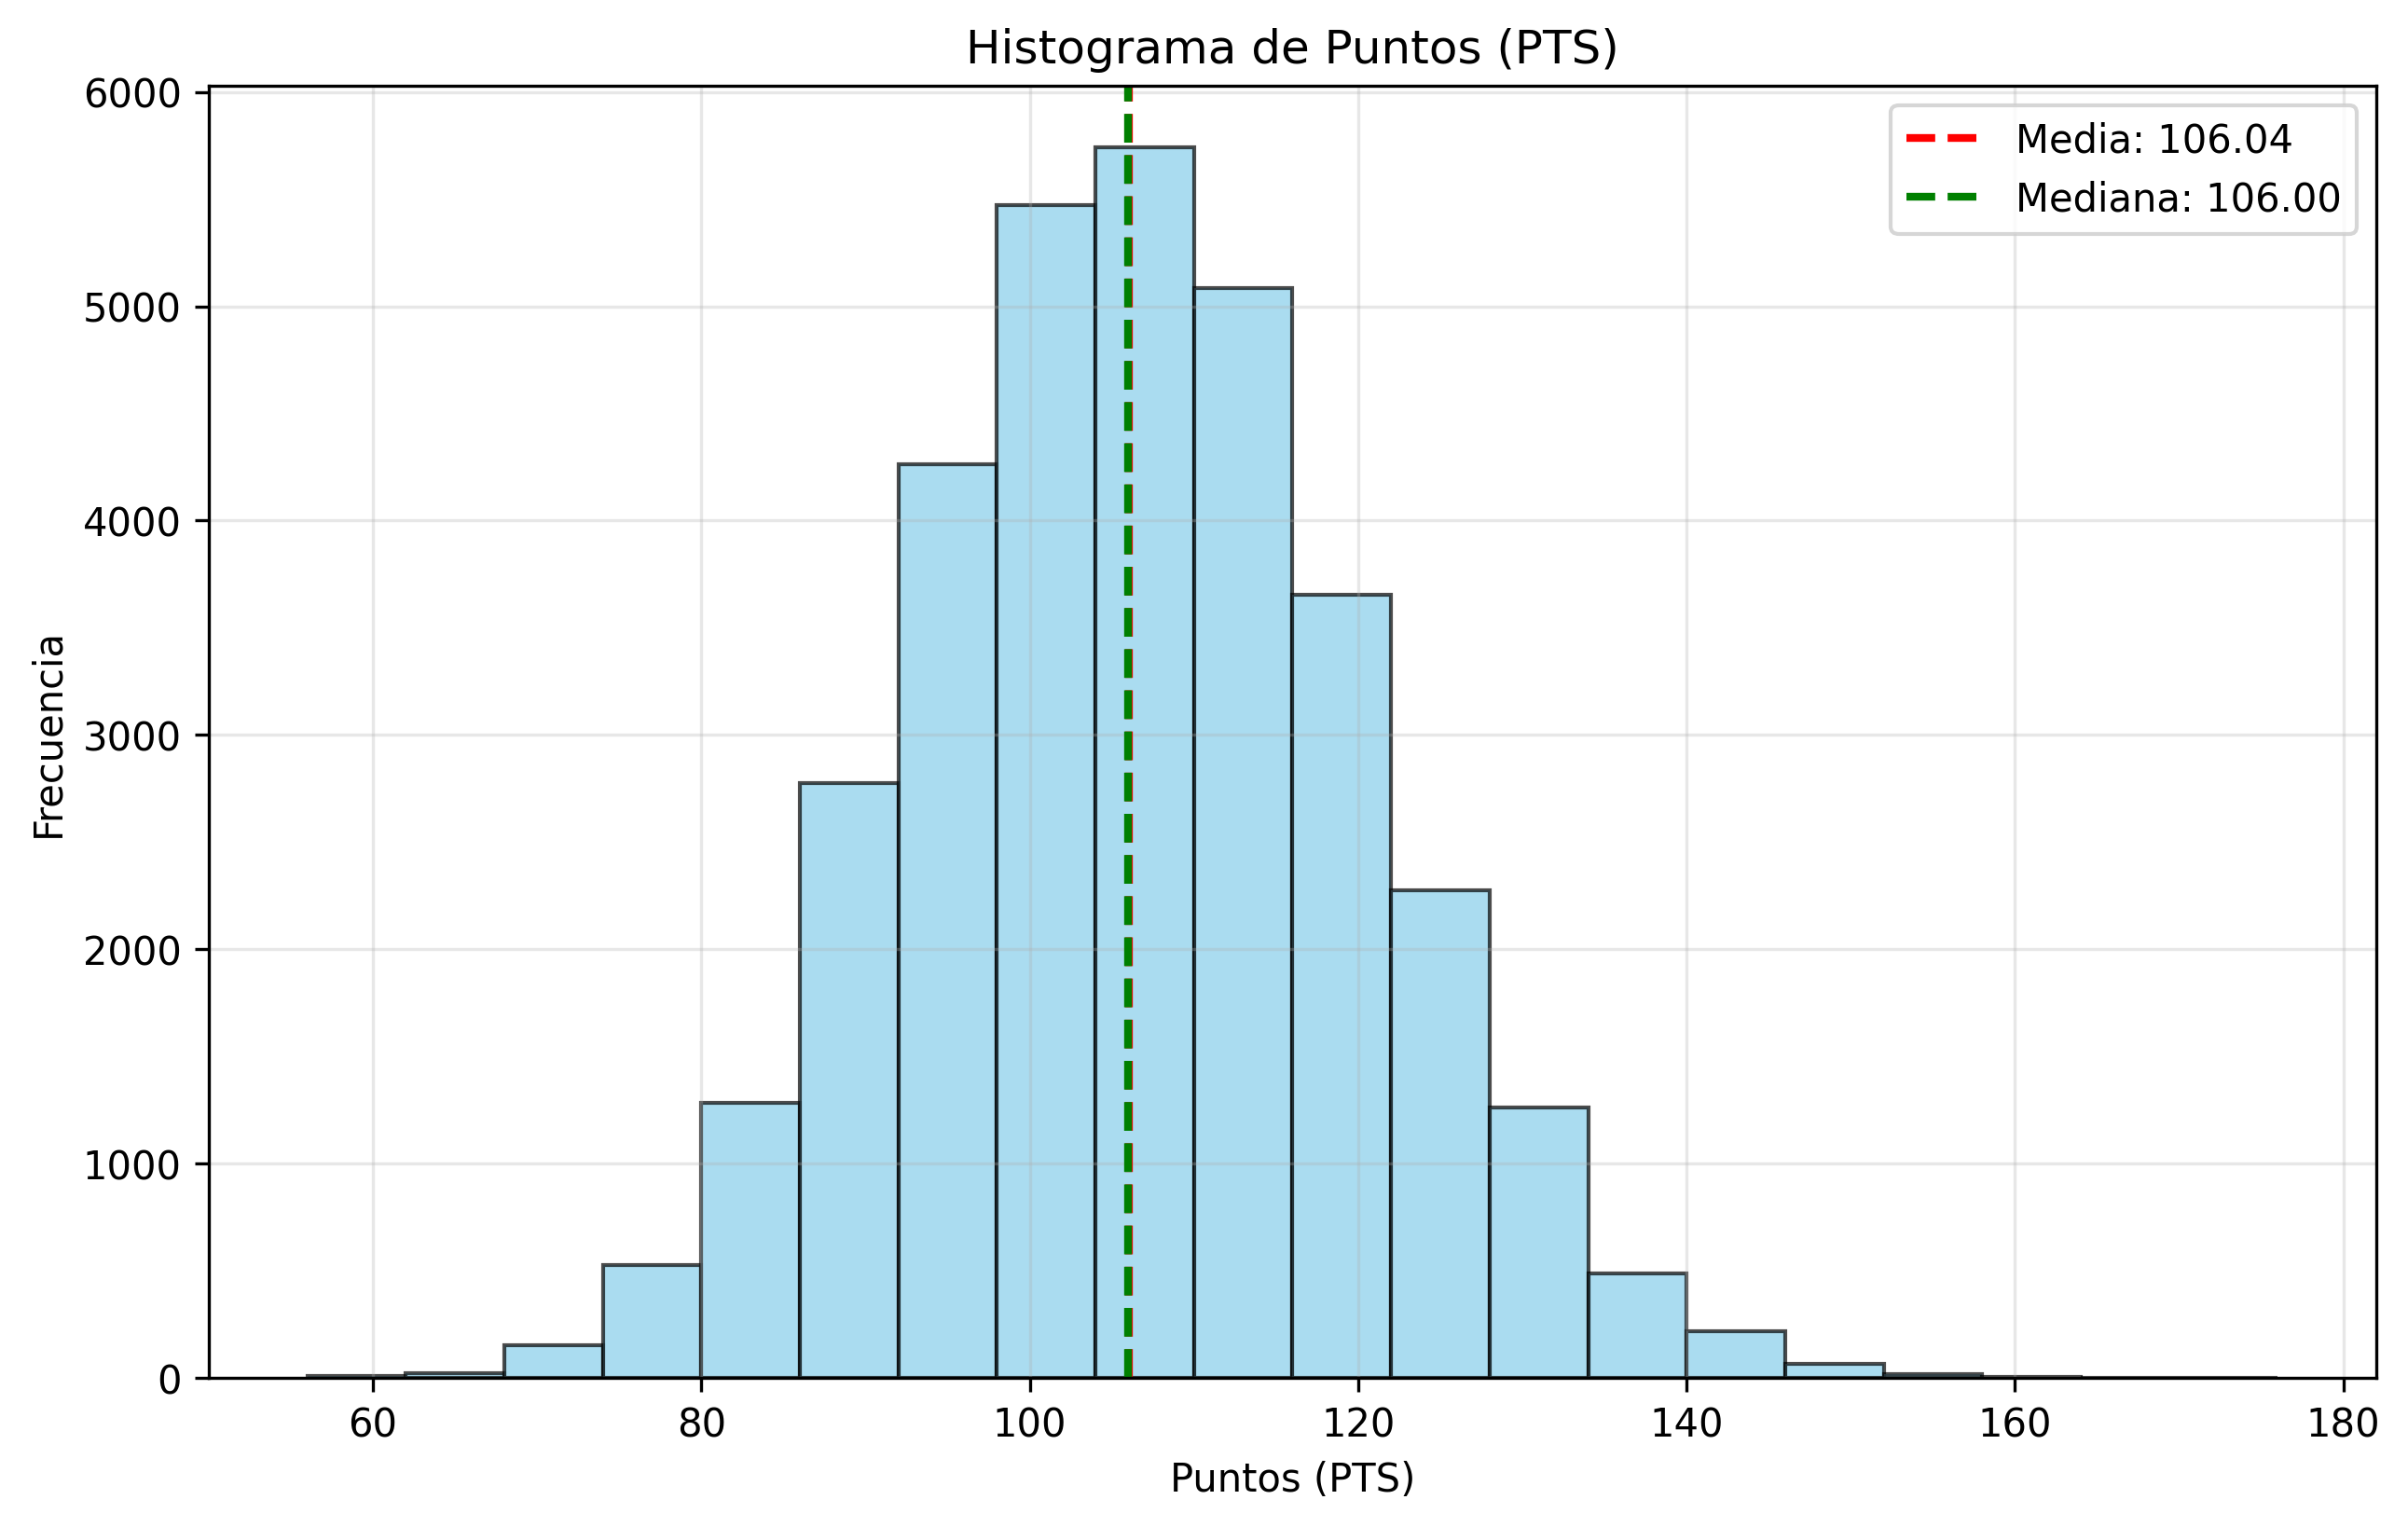
\includegraphics[width=\linewidth]{images/histograma_pts.png}
\caption{Histograma de Puntos Totales (PTS). Media: 106.04, Mediana: 106.00}
\label{fig:hist_pts}
\end{minipage}
\hfill
\begin{minipage}{0.48\textwidth}
\centering
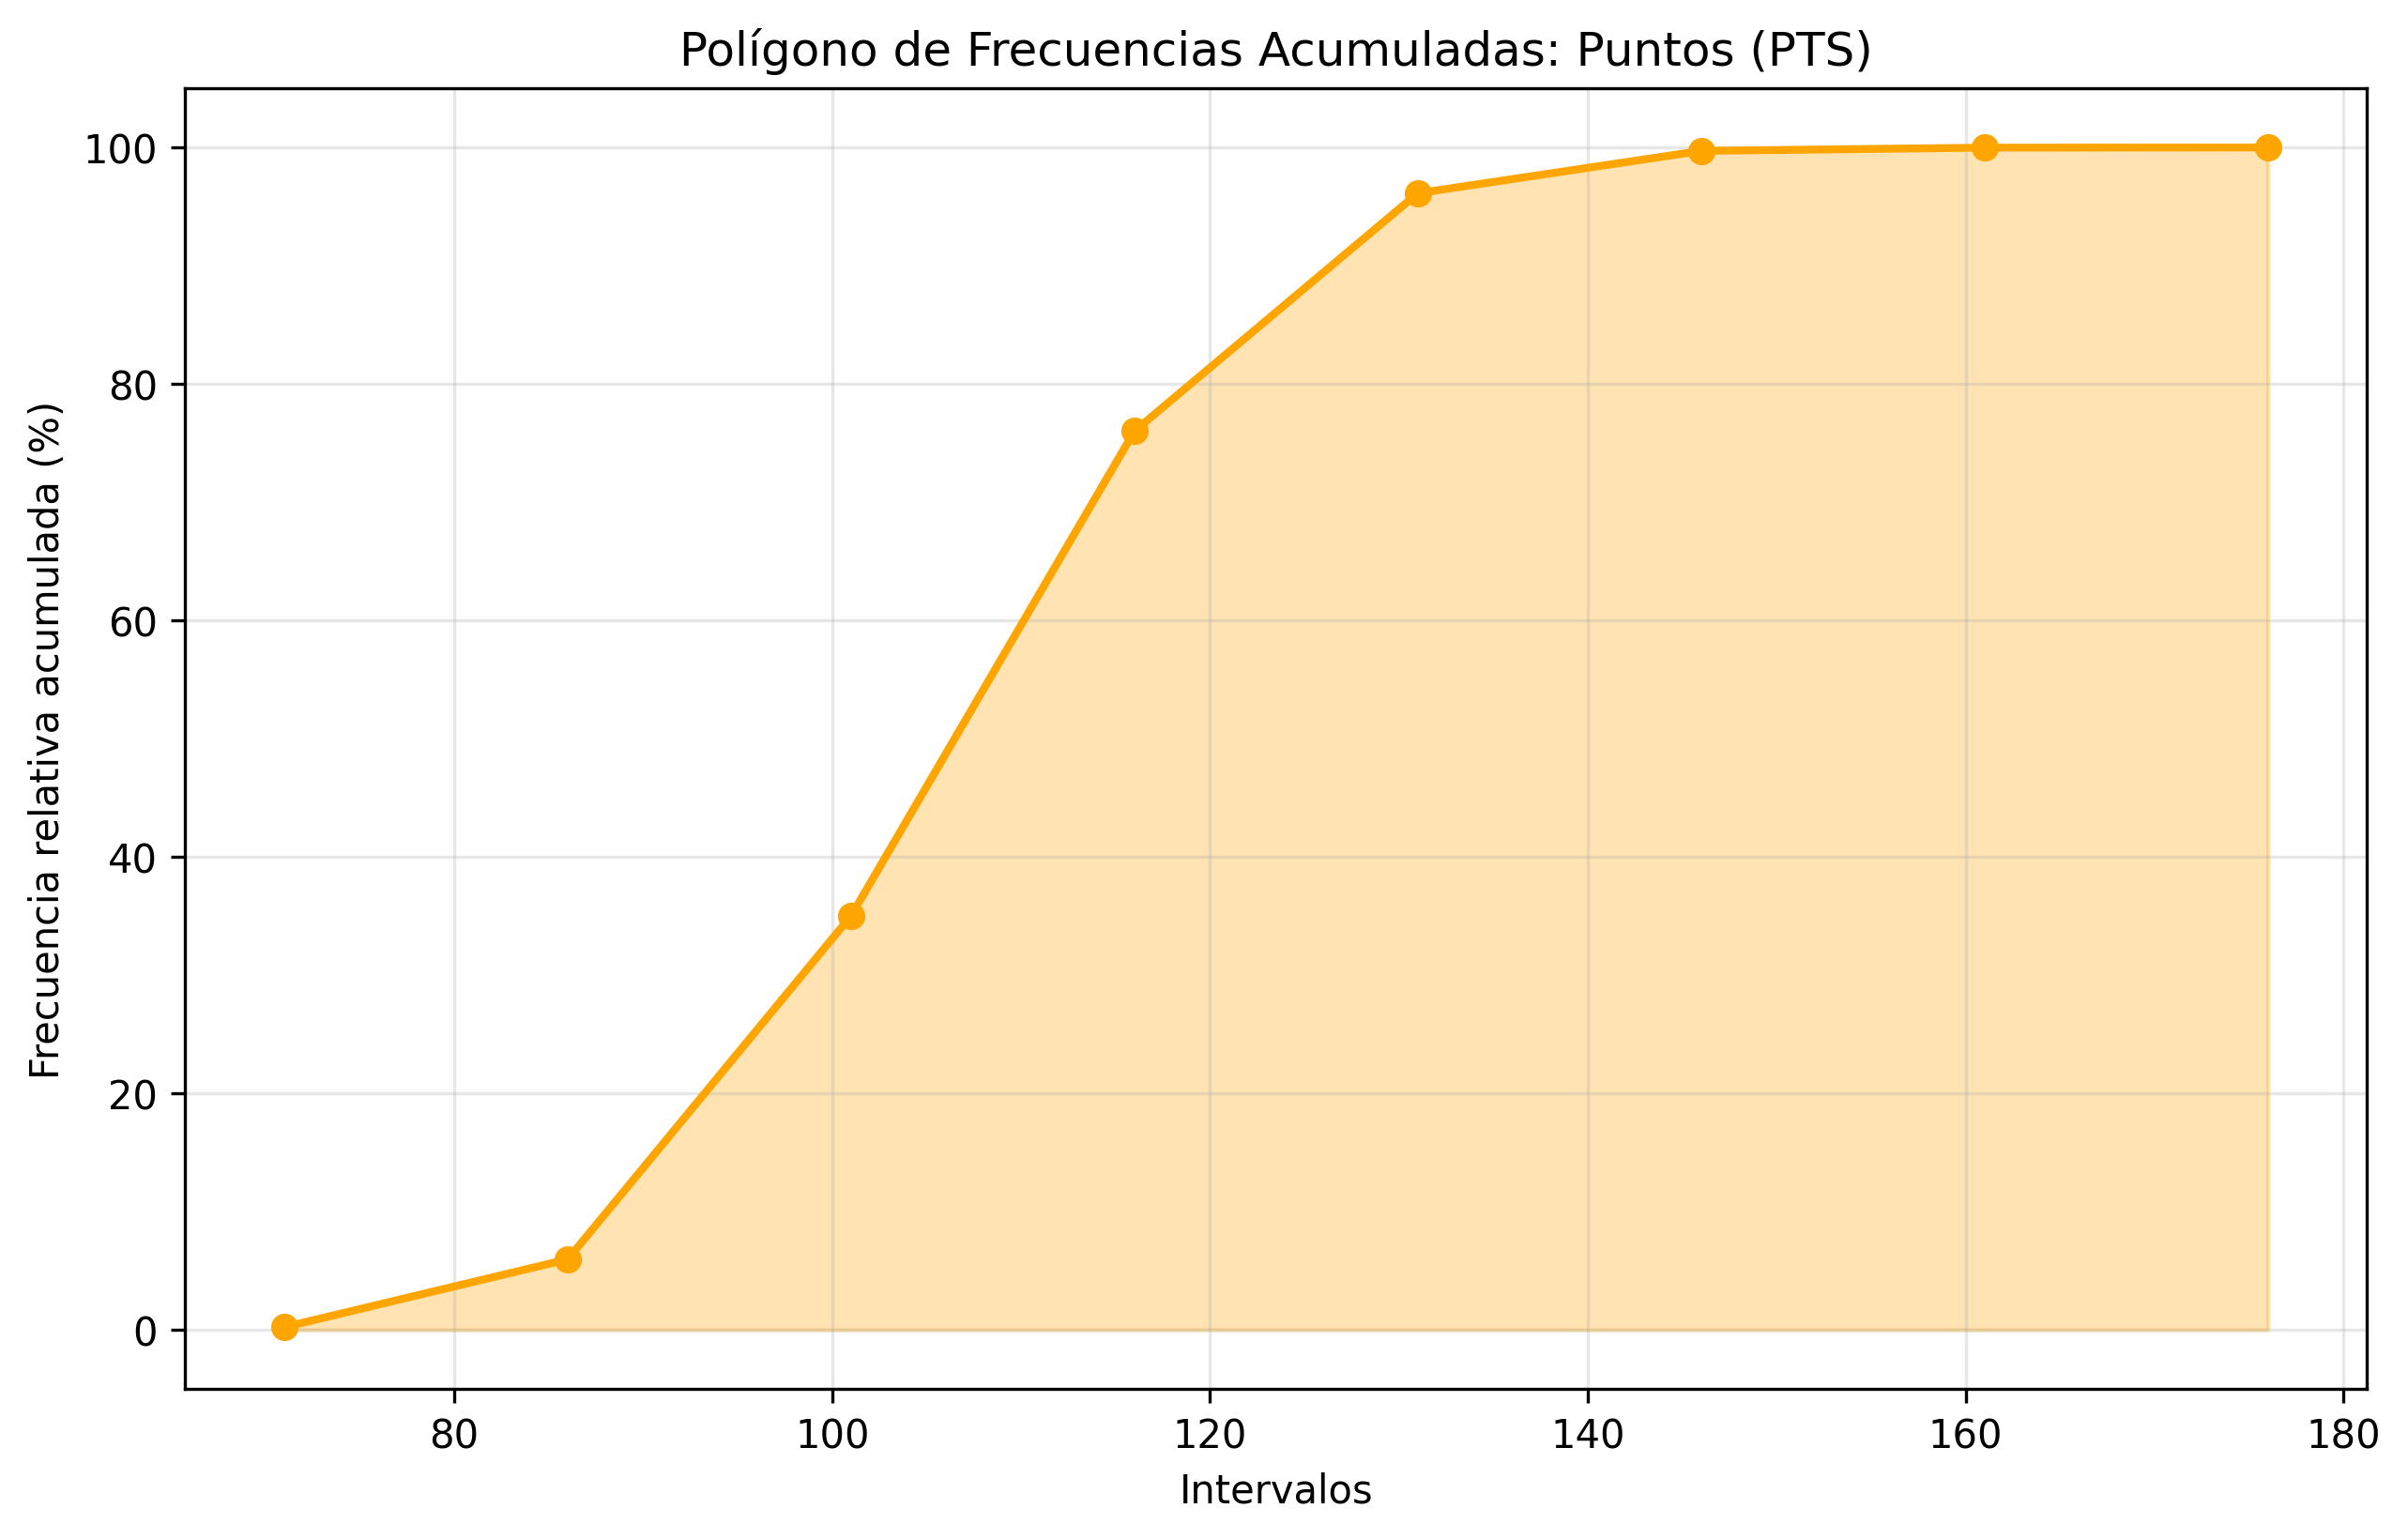
\includegraphics[width=\linewidth]{images/poligono_acumulado_pts.png}
\caption{Polígono acumulado de PTS}
\label{fig:pol_pts}
\end{minipage}
\end{figure}

\begin{figure}[H]
\centering
\begin{minipage}{0.48\textwidth}
\centering
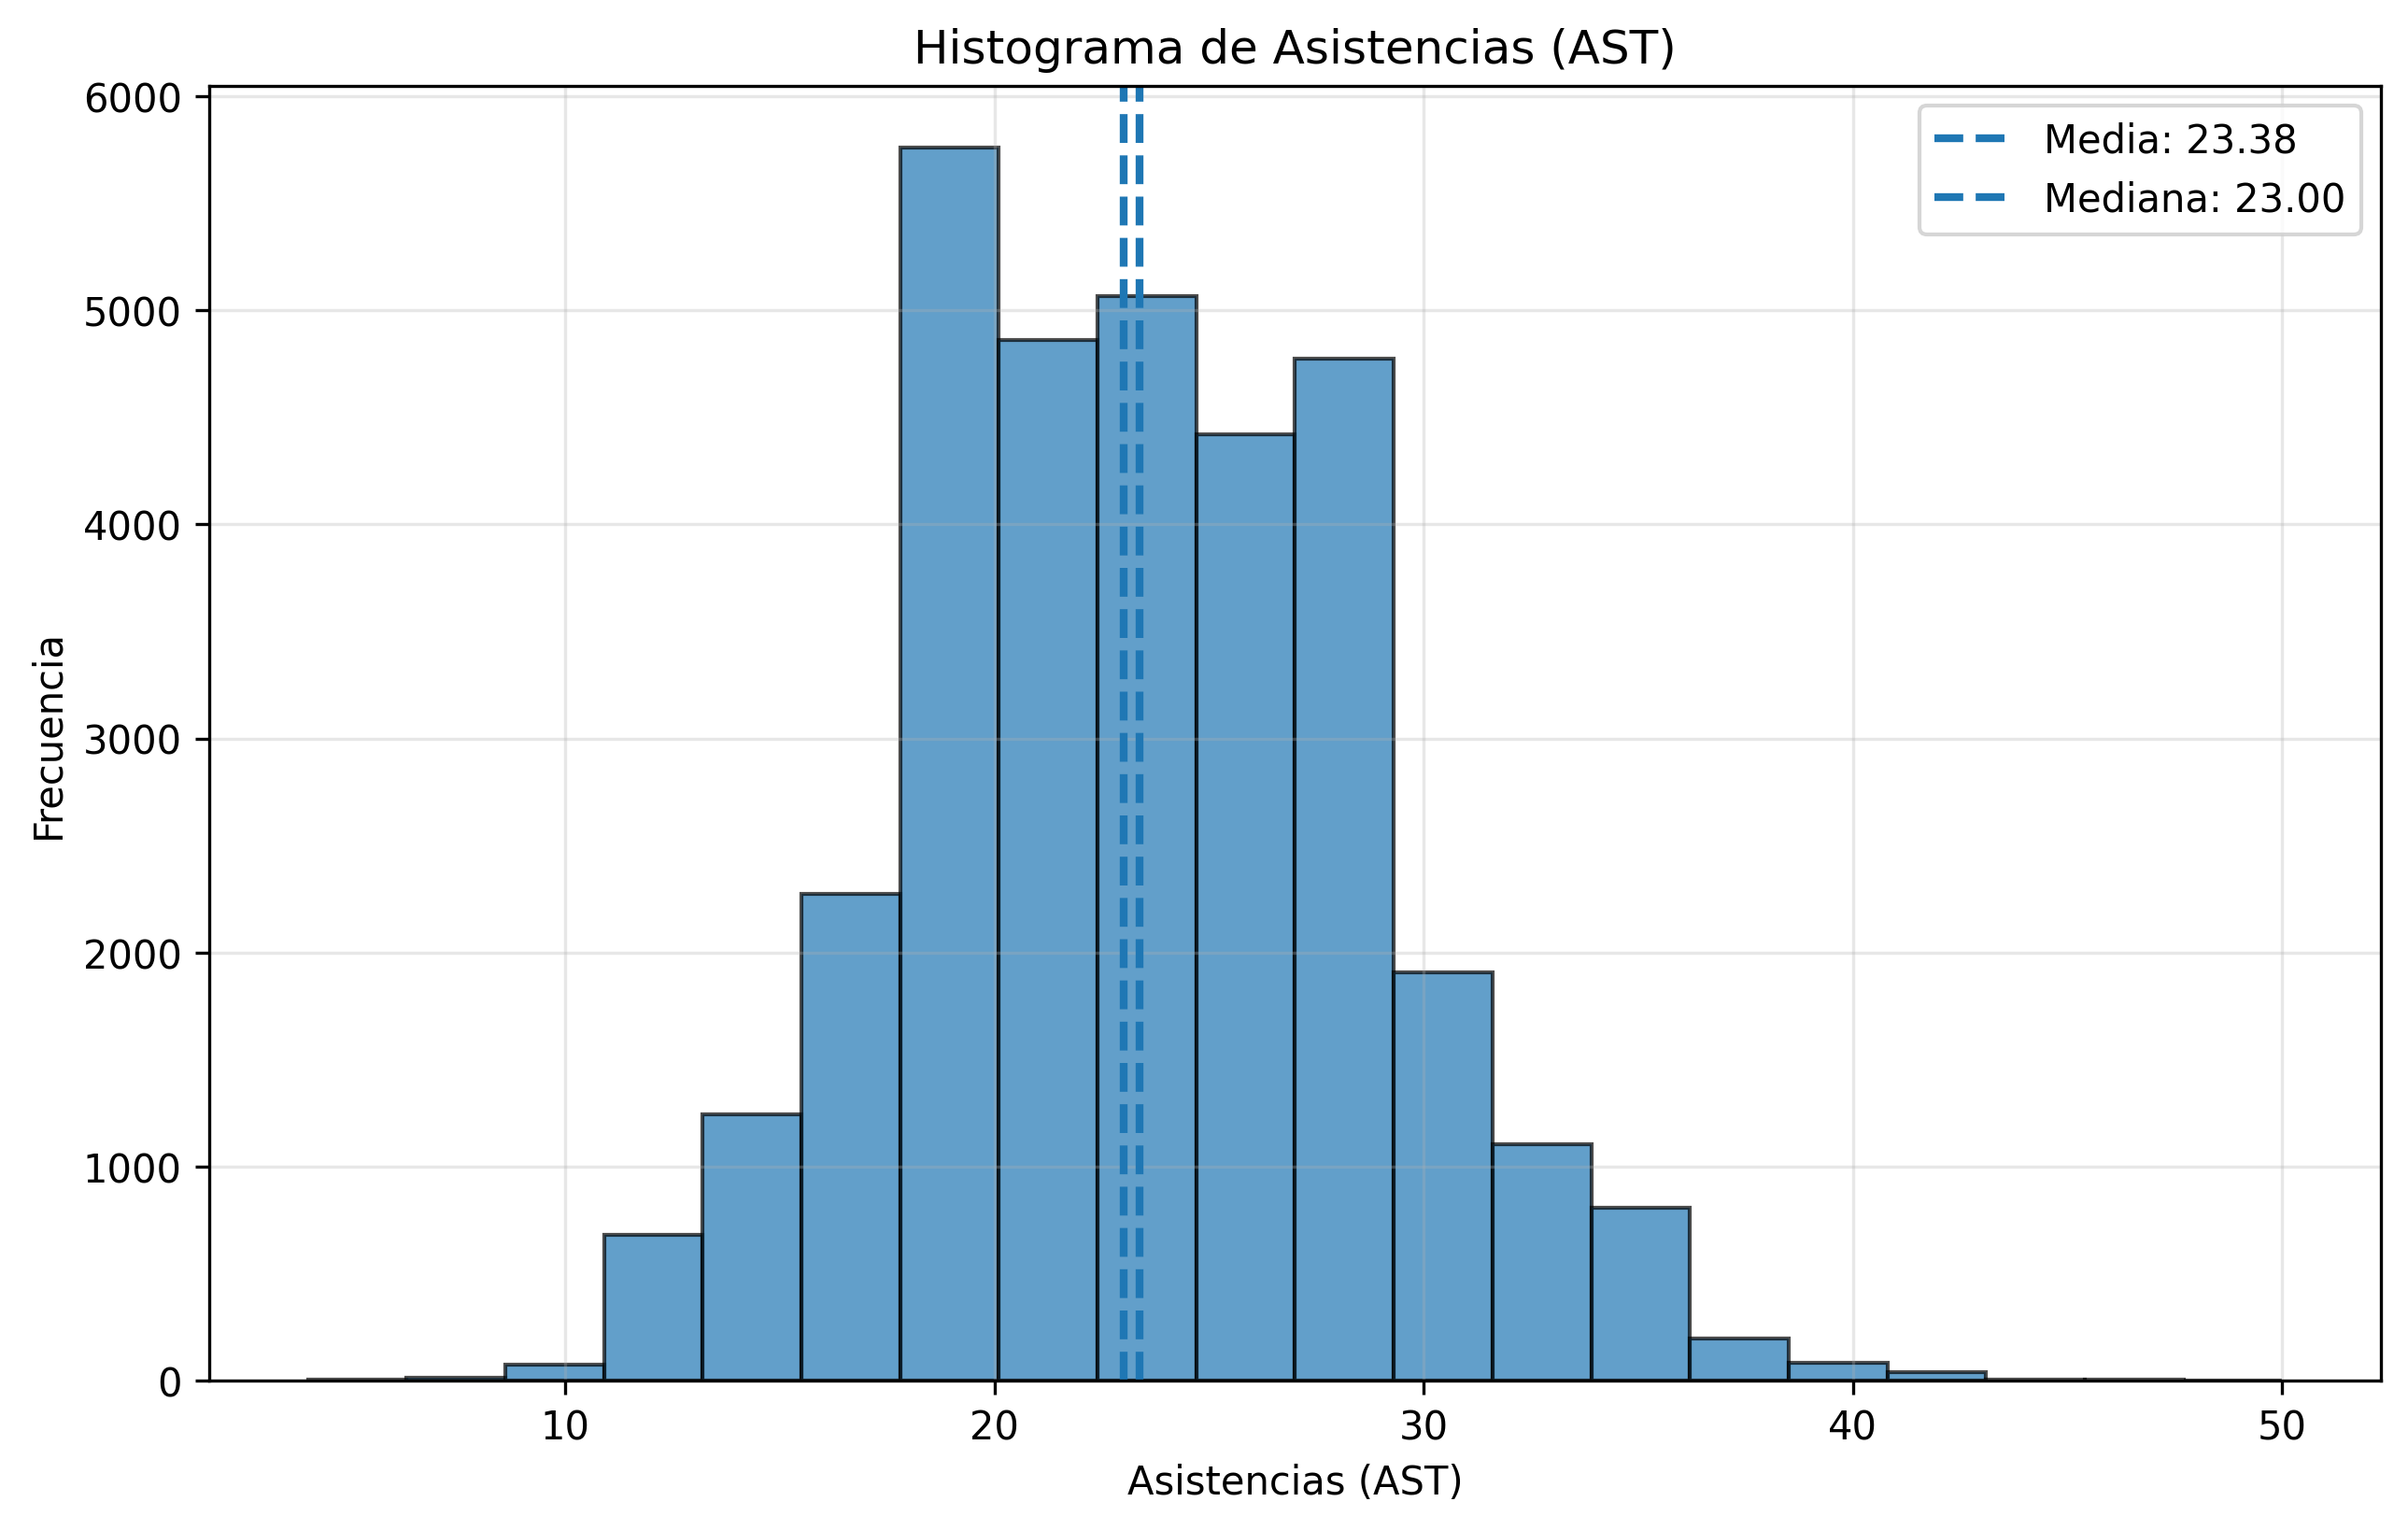
\includegraphics[width=\linewidth]{images/histograma_ast.png}
\caption{Histograma de Asistencias (AST). Media: 23.38, Mediana: 23.00}
\label{fig:hist_ast}
\end{minipage}
\hfill
\begin{minipage}{0.48\textwidth}
\centering
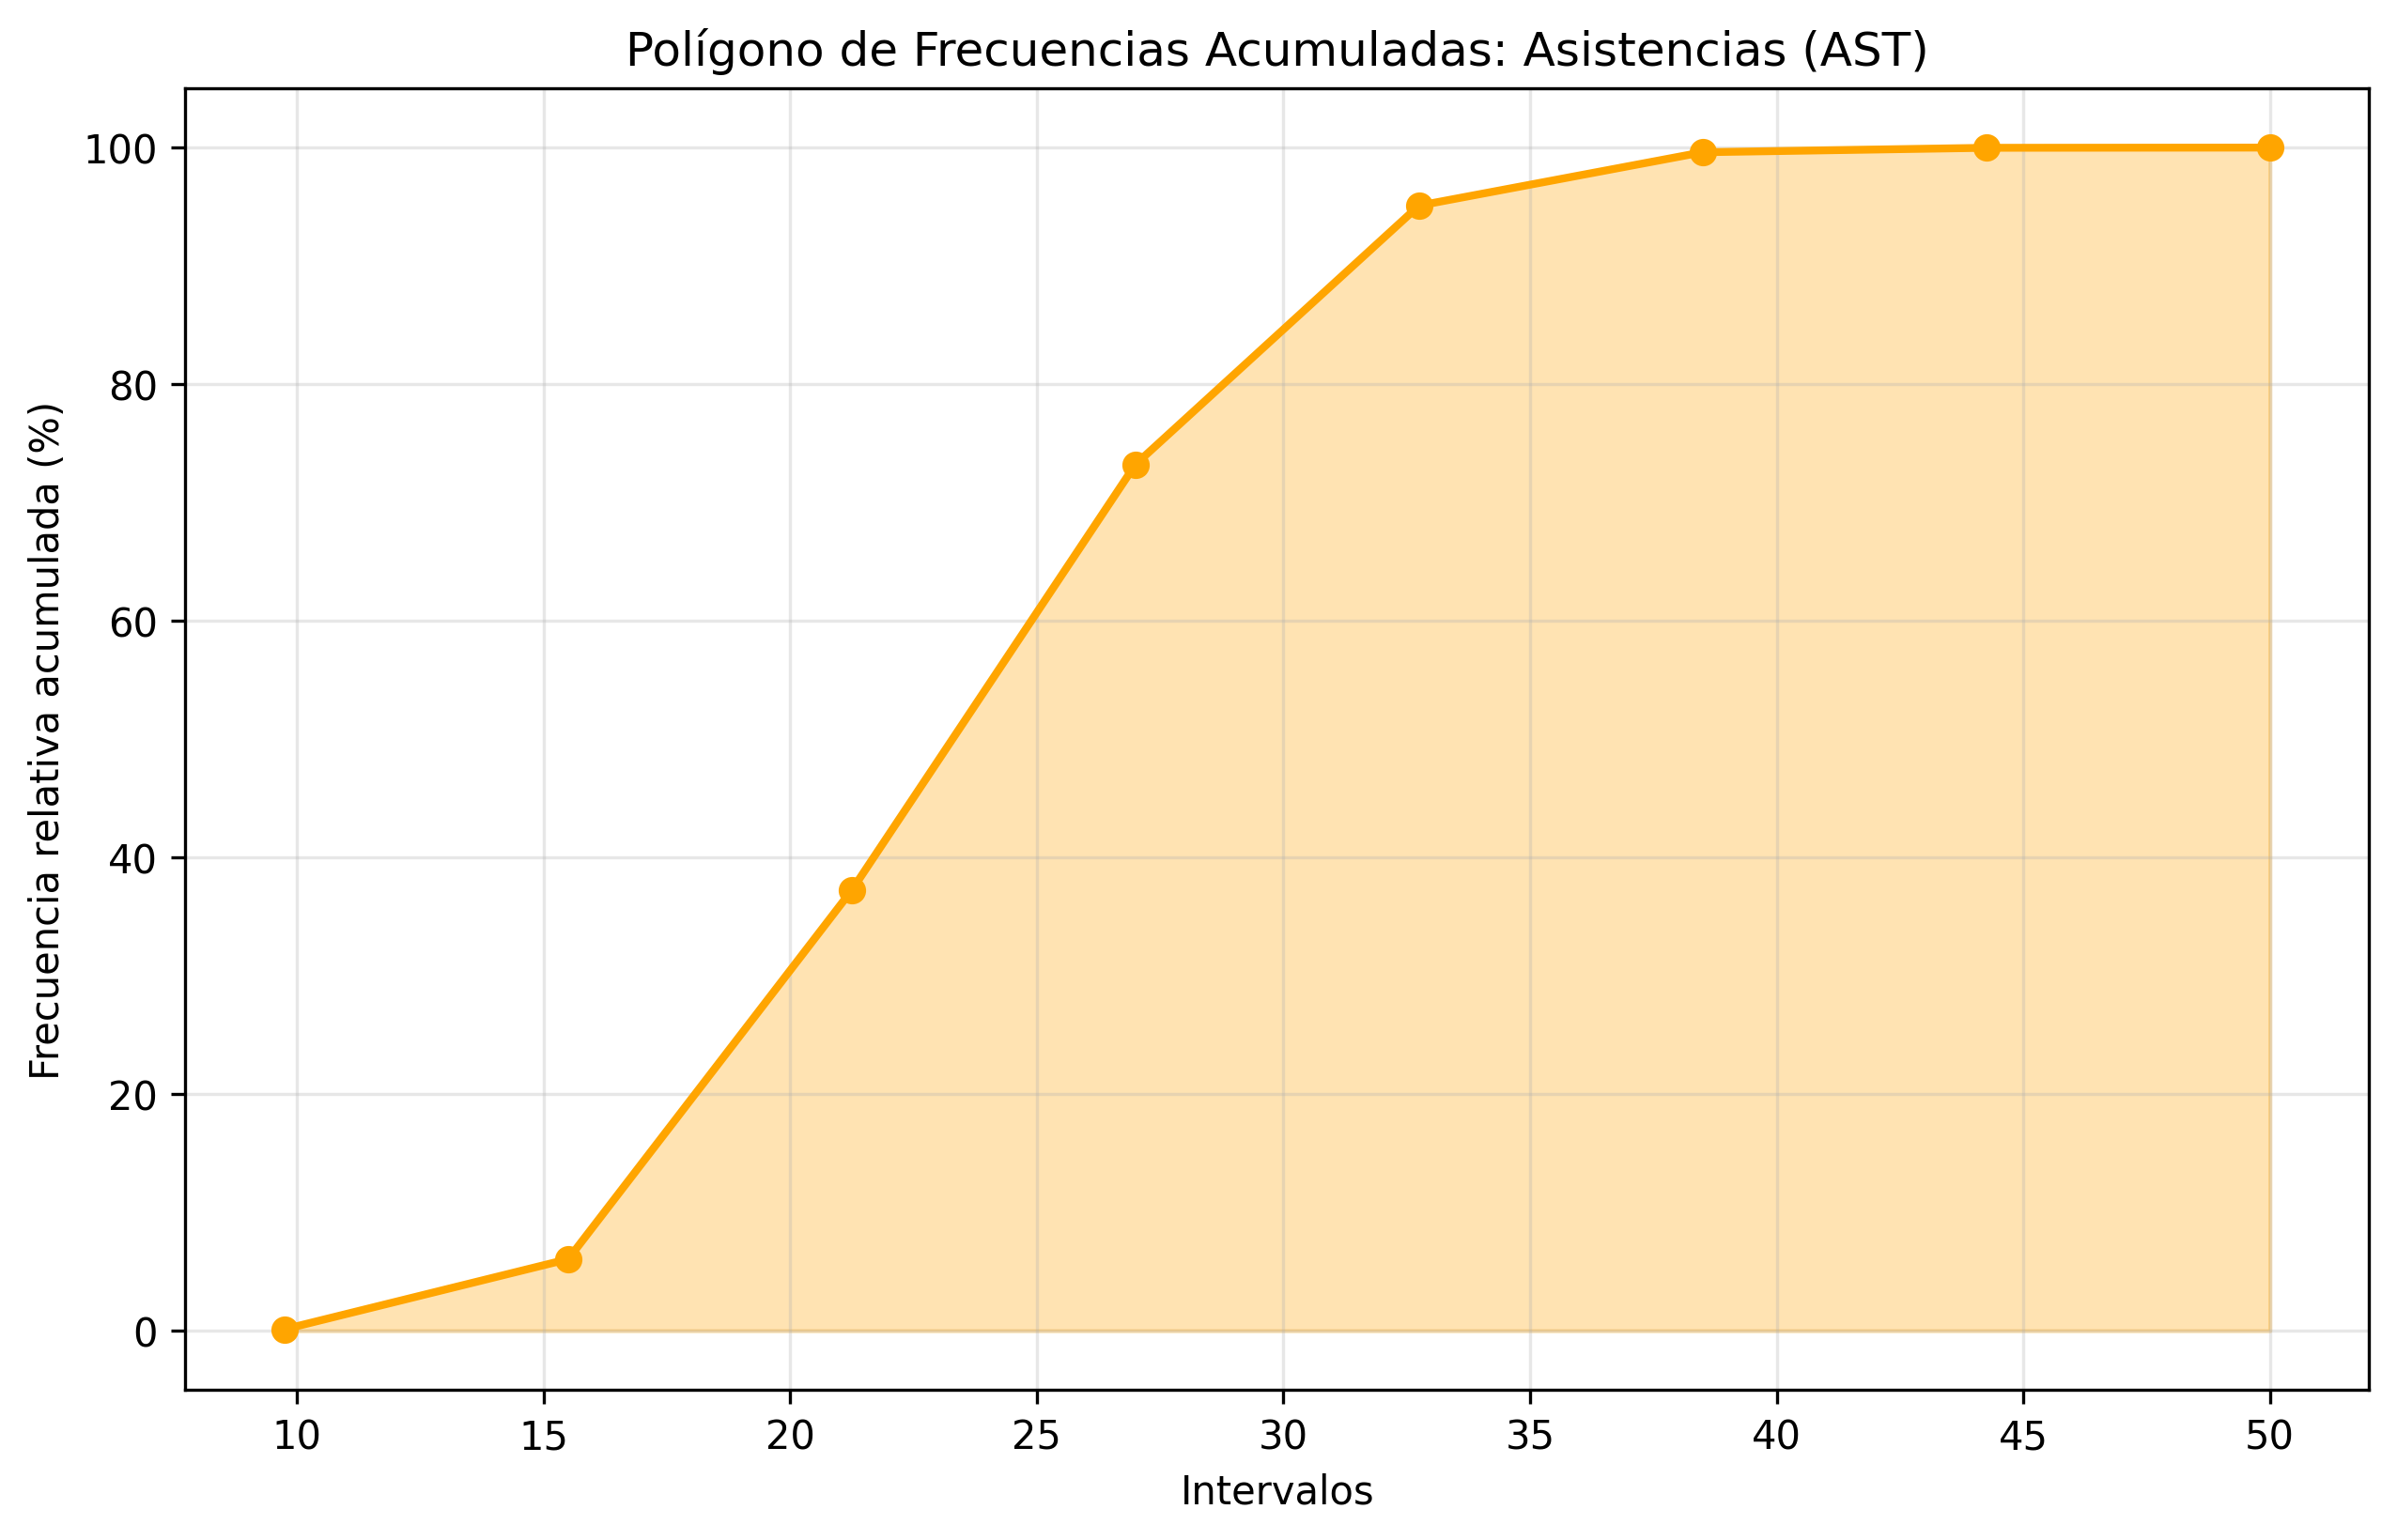
\includegraphics[width=\linewidth]{images/poligono_acumulado_ast.png}
\caption{Polígono acumulado de Asistencias (AST)}
\label{fig:pol_ast}
\end{minipage}
\end{figure}

\begin{figure}[H]
\centering
\begin{minipage}{0.48\textwidth}
\centering
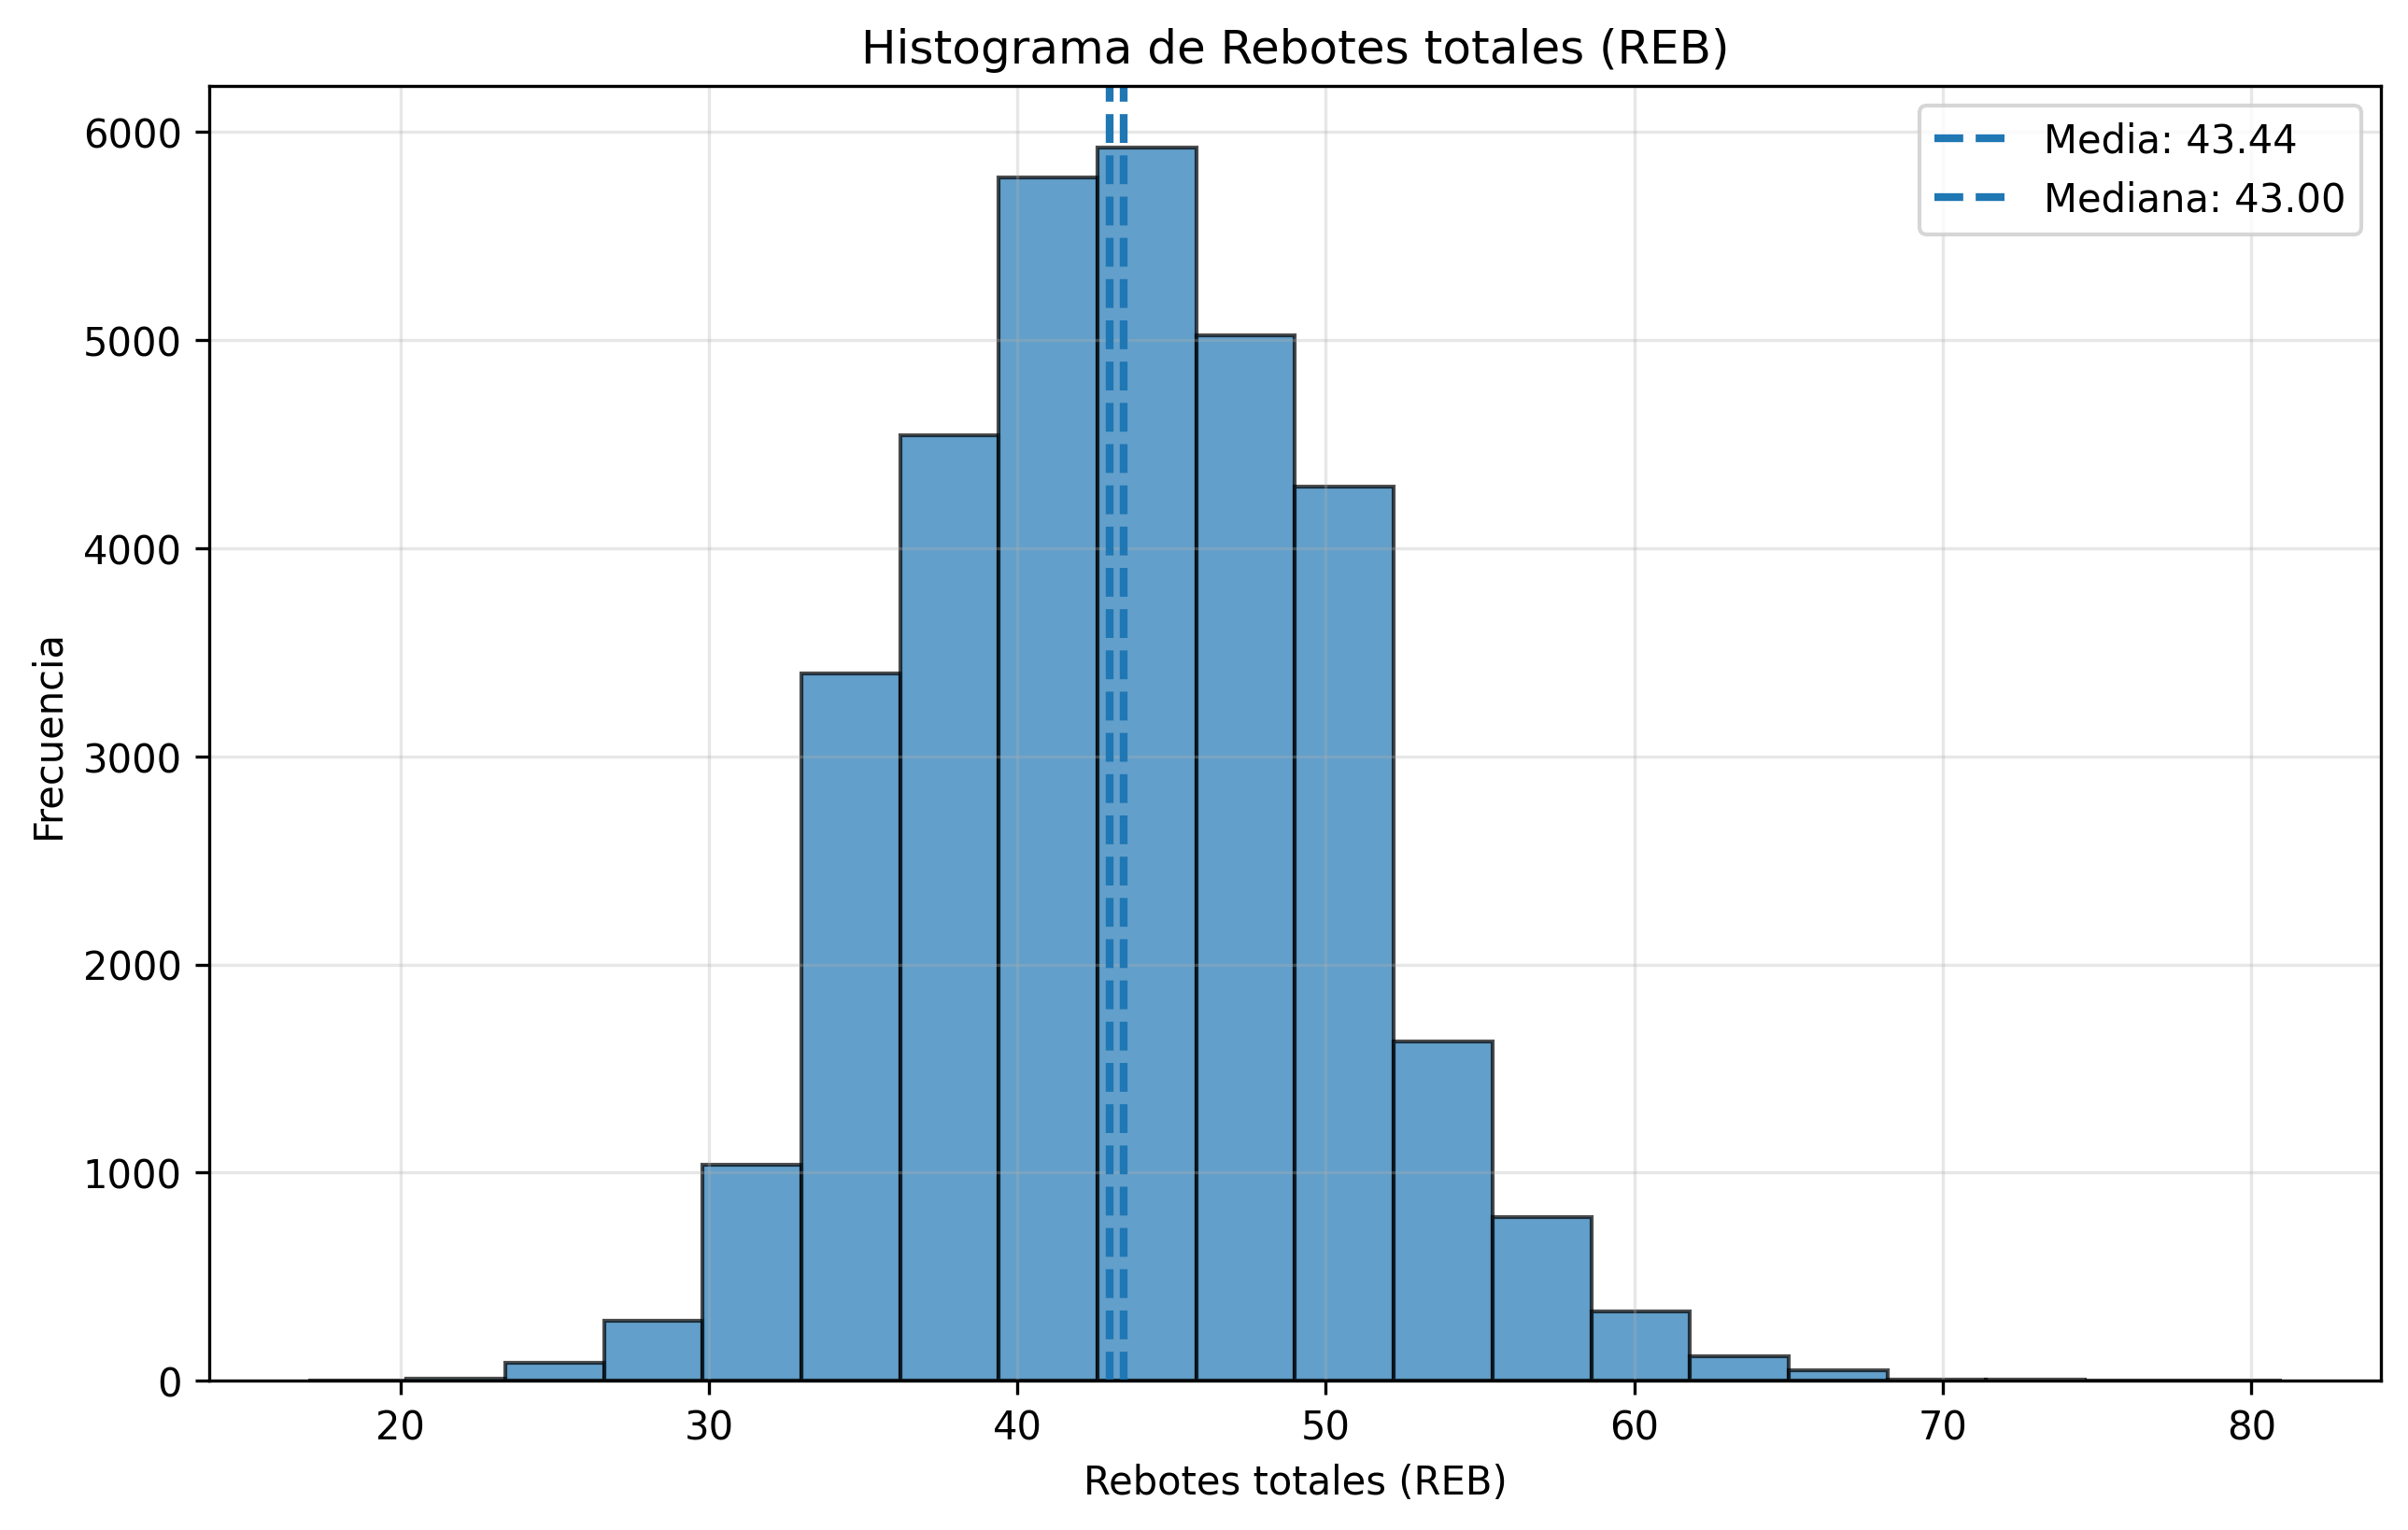
\includegraphics[width=\linewidth]{images/histograma_reb.png}
\caption{Histograma de Rebotes Totales (REB). Media: 43.44, Mediana: 43.00}
\label{fig:hist_reb}
\end{minipage}
\hfill
\begin{minipage}{0.48\textwidth}
\centering
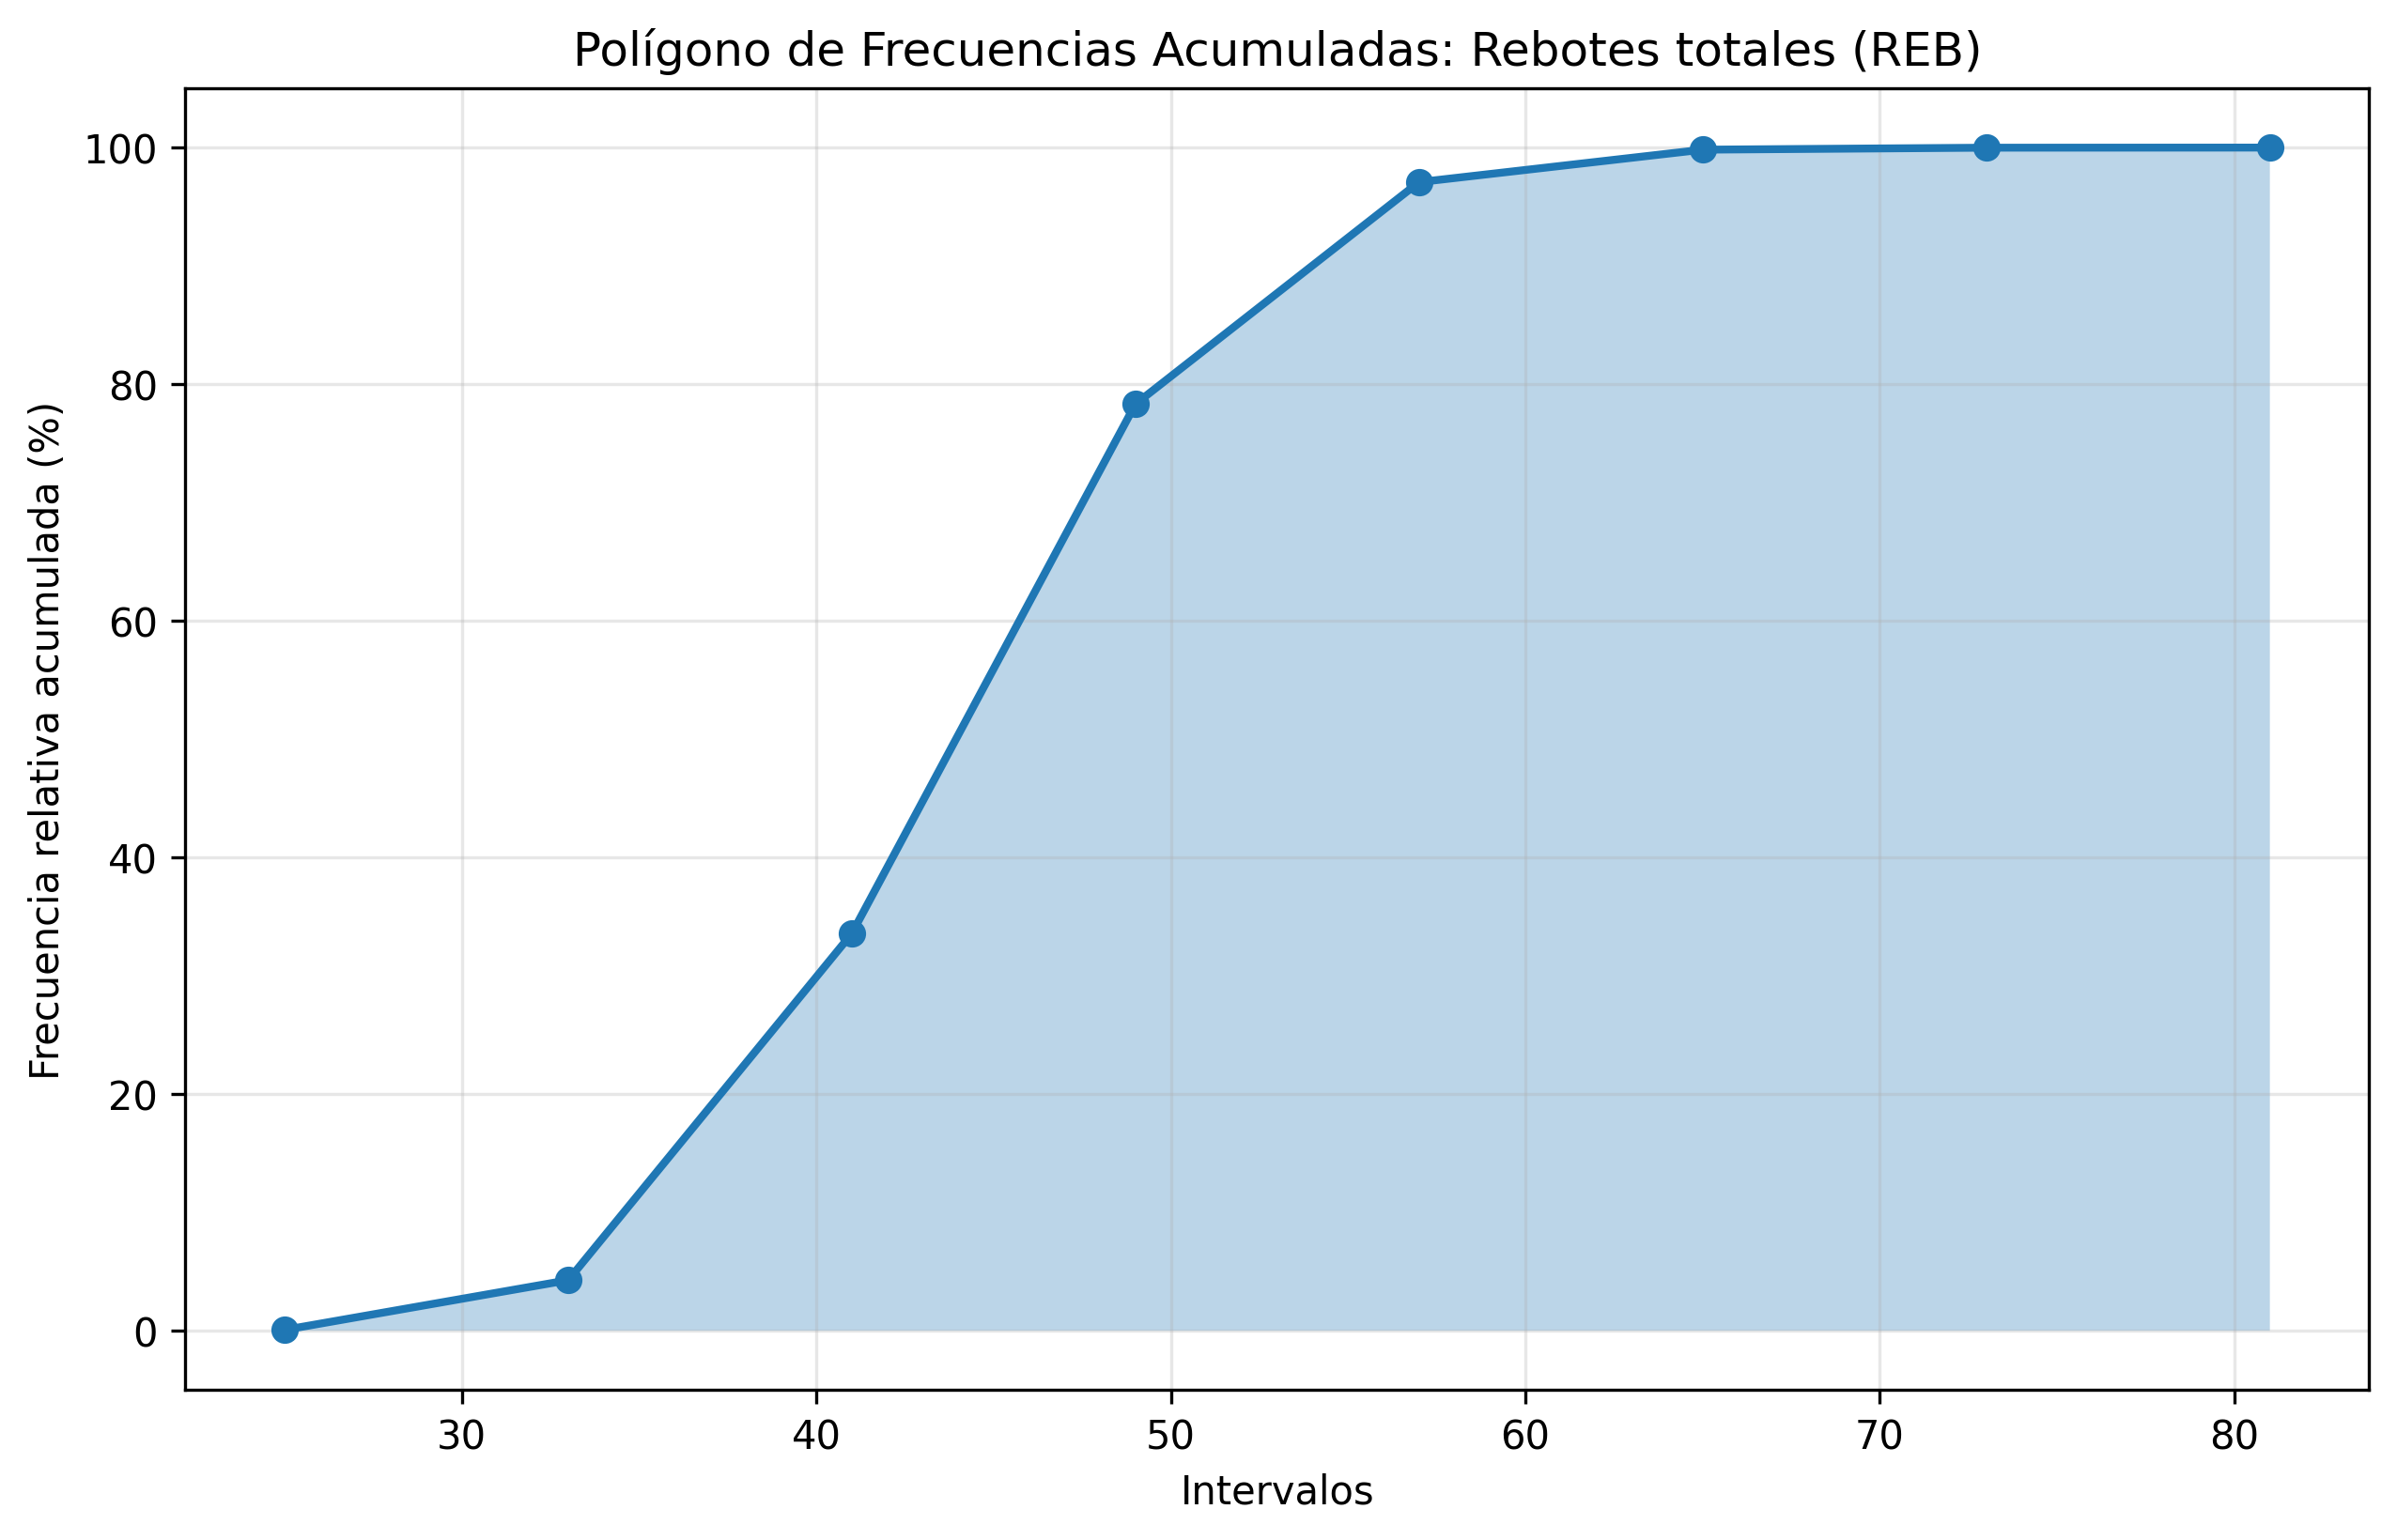
\includegraphics[width=\linewidth]{images/poligono_acumulado_reb.png}
\caption{Polígono acumulado de REB}
\label{fig:pol_reb}
\end{minipage}
\end{figure}

\subsection*{Variables restantes}
Dada la diversidad en la forma, dispersión y significado estadístico de estas variables, se
realiza un análisis gráfico individual para cada una. Este enfoque permite capturar las
particularidades de sus distribuciones y resaltar aquellos rasgos que resultan relevantes para la
interpretación del juego y para su incorporación en modelos estadísticos posteriores.

\subsubsection*{Distribución del Porcentaje de Triples (FG3\_PCT)}

\begin{figure}[H]
\centering
\begin{minipage}{0.48\textwidth}
\centering
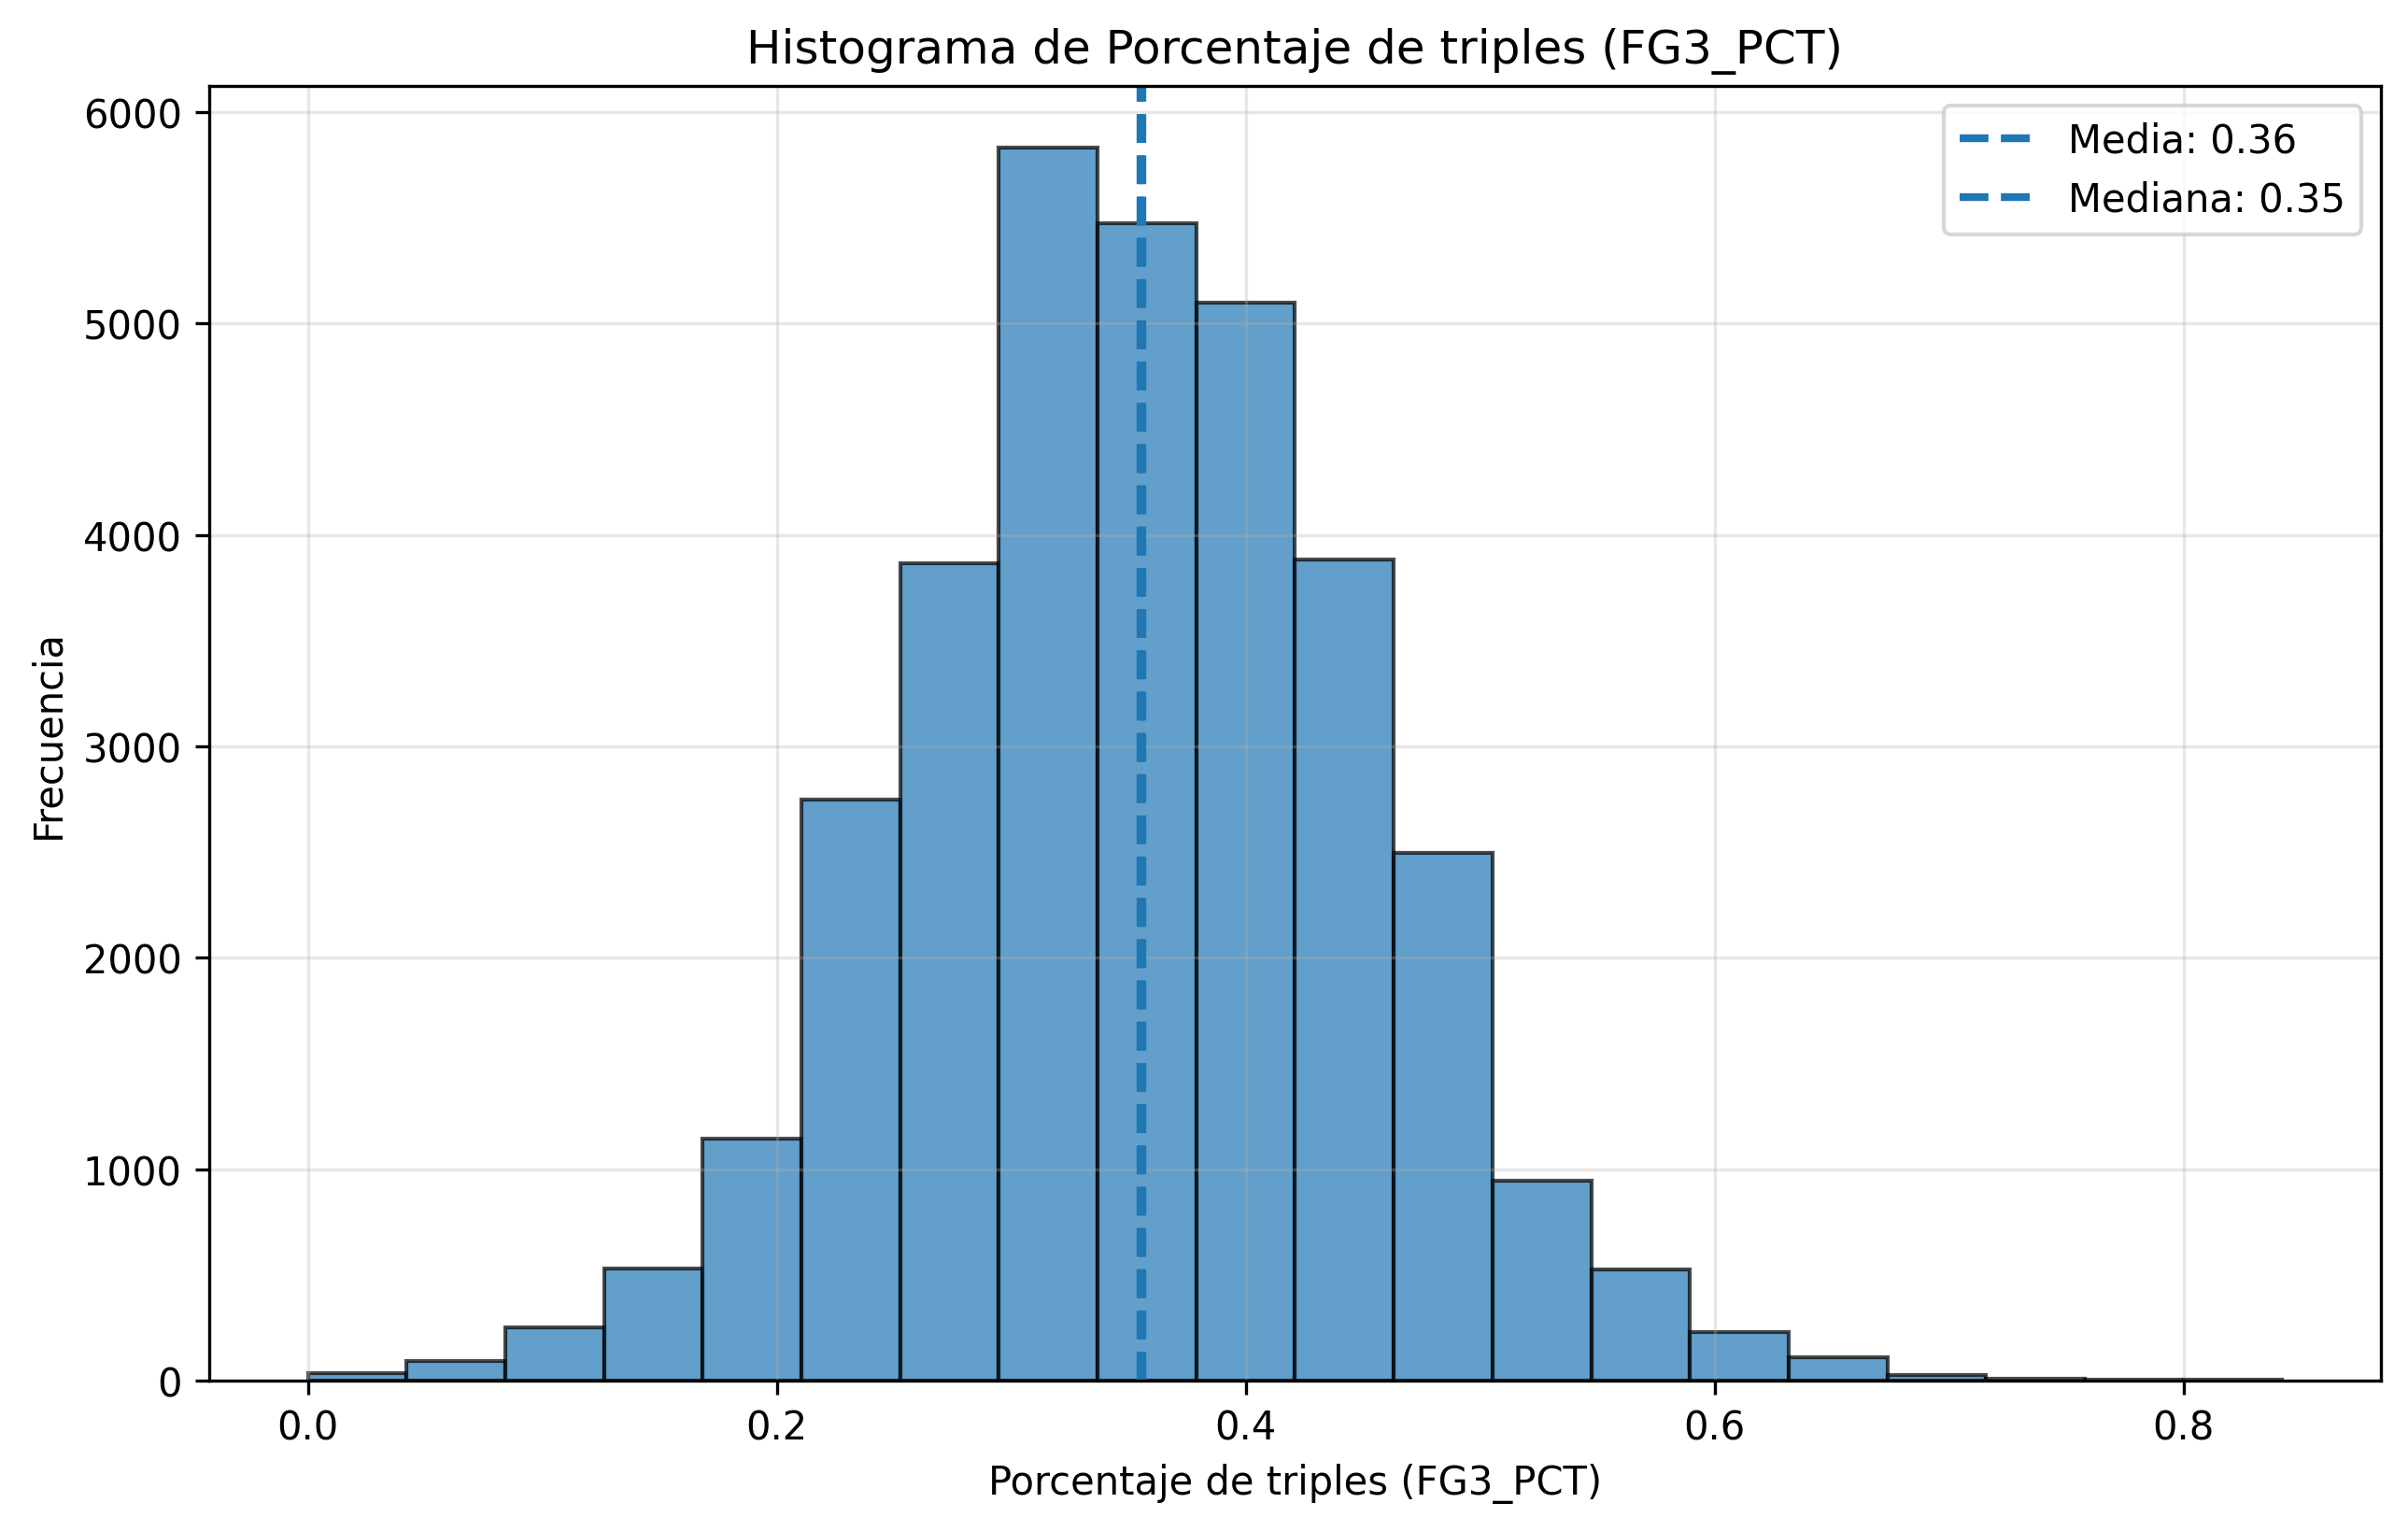
\includegraphics[width=\linewidth]{images/histograma_fg3_pct.png}
\caption{Histograma de Porcentaje de Triples (FG3\_PCT)}
\label{fig:hist_fg3_pct}
\end{minipage}
\hfill
\begin{minipage}{0.48\textwidth}
\centering
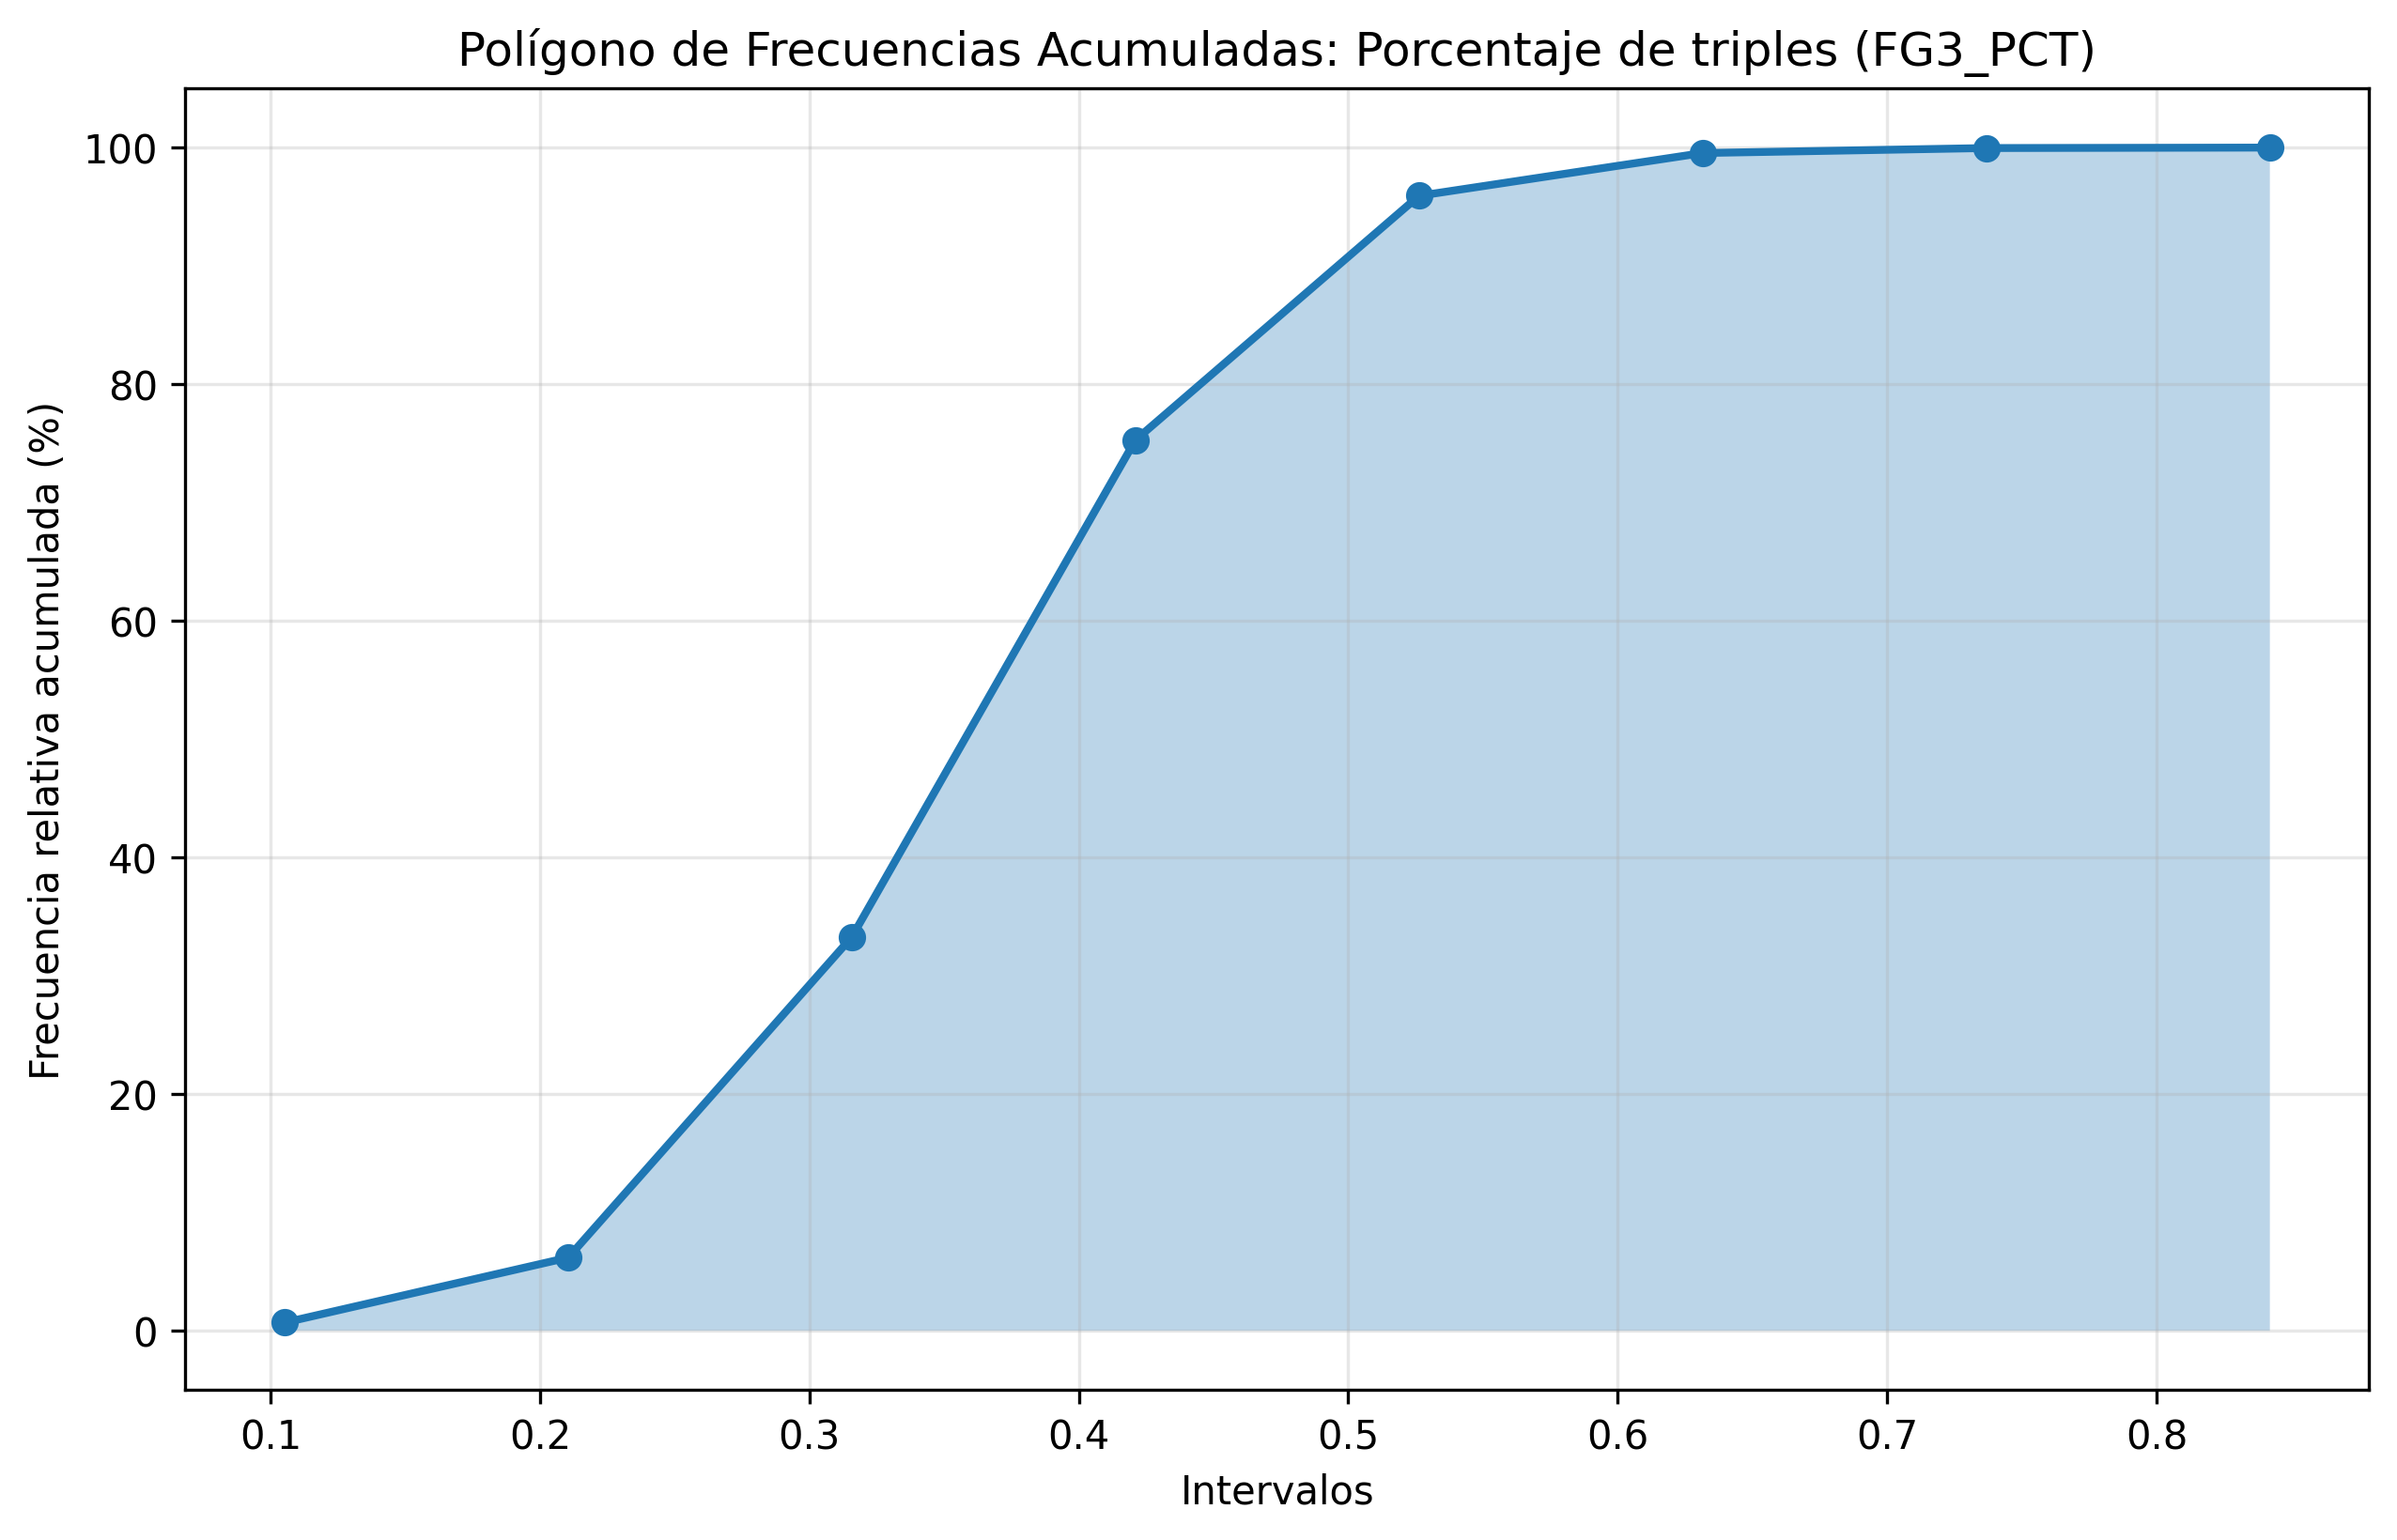
\includegraphics[width=\linewidth]{images/poligono_acumulado_fg3_pct.png}
\caption{Polígono acumulado de FG3\%}
\label{fig:pol_fg3_pct}
\end{minipage}
\end{figure}

El porcentaje de triples presenta una distribución aproximadamente normal con centro alrededor del 35\%-40\%. La distribución es más dispersa que la de tiros de campo generales, reflejando la mayor variabilidad inherente al tiro de tres puntos. La simetría observada sugiere que los valores extremos (tanto muy bajos como muy altos) son igualmente probables. El polígono acumulado muestra una curva en forma de S suave, confirmando la naturaleza simétrica de la distribución, con aproximadamente el 50\% de los partidos registrando un porcentaje inferior al 40\%.

\subsubsection*{Distribución del Porcentaje de Tiros Libres (FT\_PCT)}

\begin{figure}[H]
\centering
\begin{minipage}{0.48\textwidth}
\centering
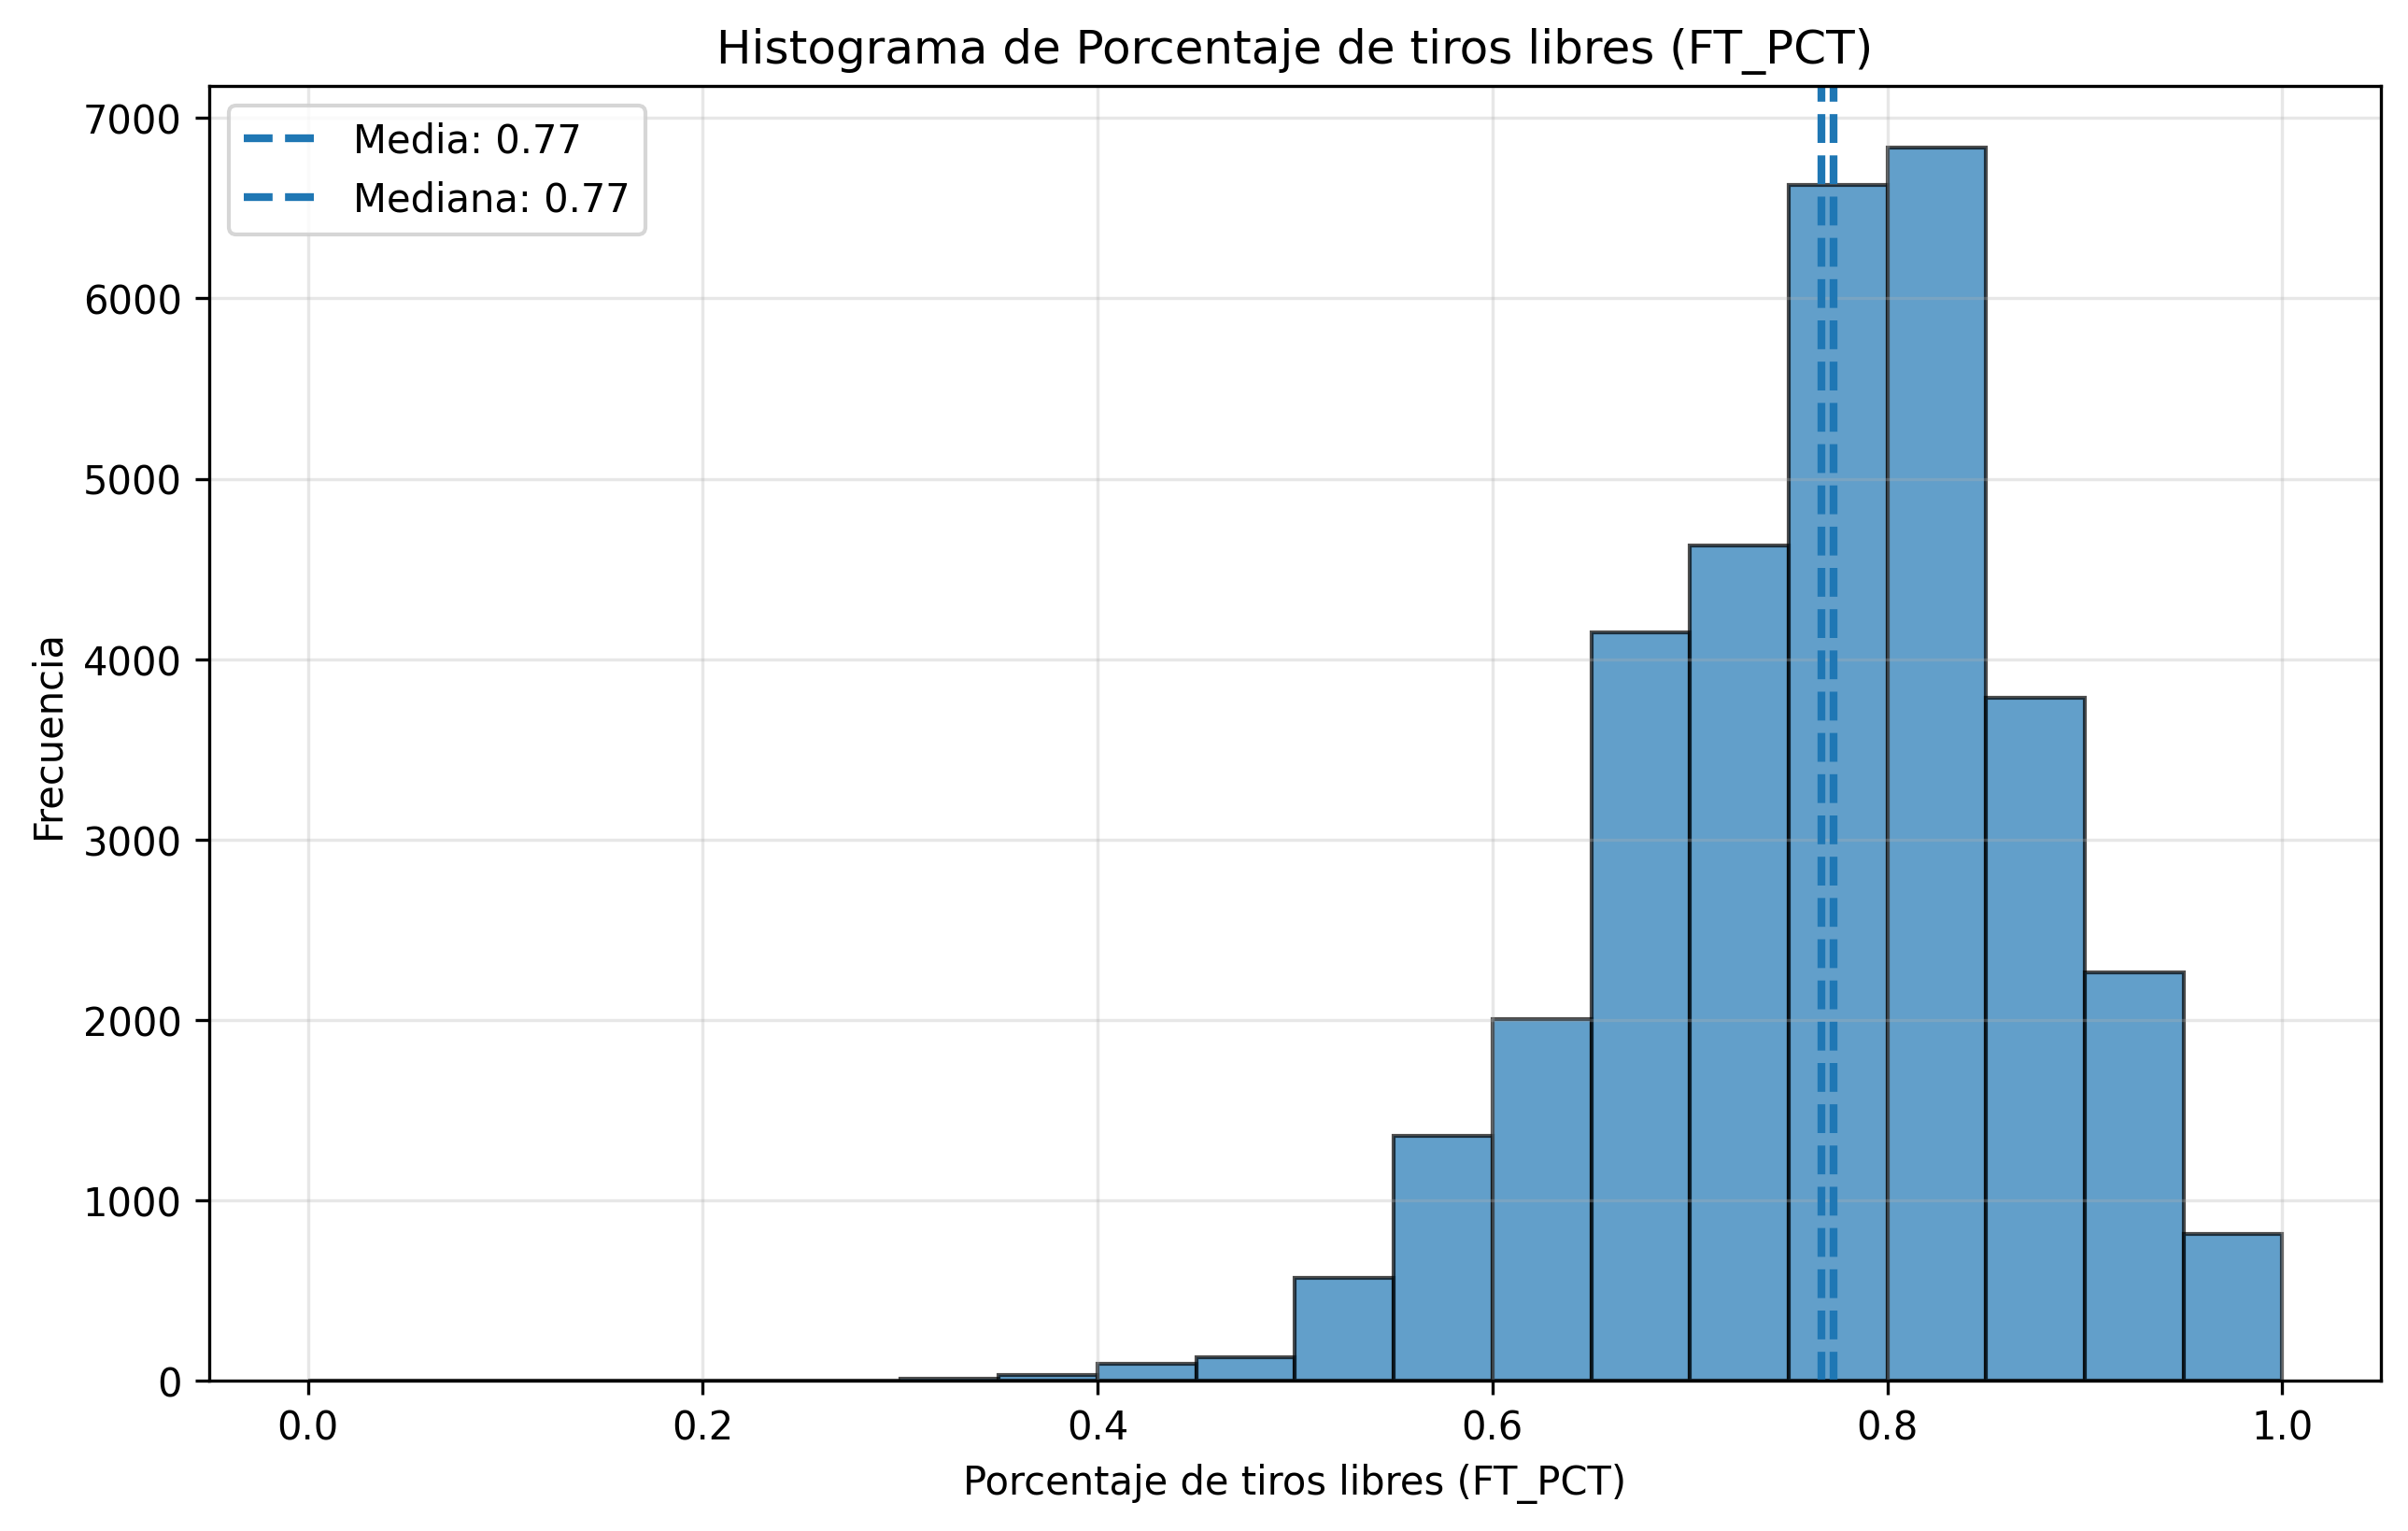
\includegraphics[width=\linewidth]{images/histograma_ft_pct.png}
\caption{Histograma de Porcentaje de Tiros Libres (FT\_PCT). Media: 0.77, Mediana: 0.77}
\label{fig:hist_ft_pct}
\end{minipage}
\hfill
\begin{minipage}{0.48\textwidth}
\centering
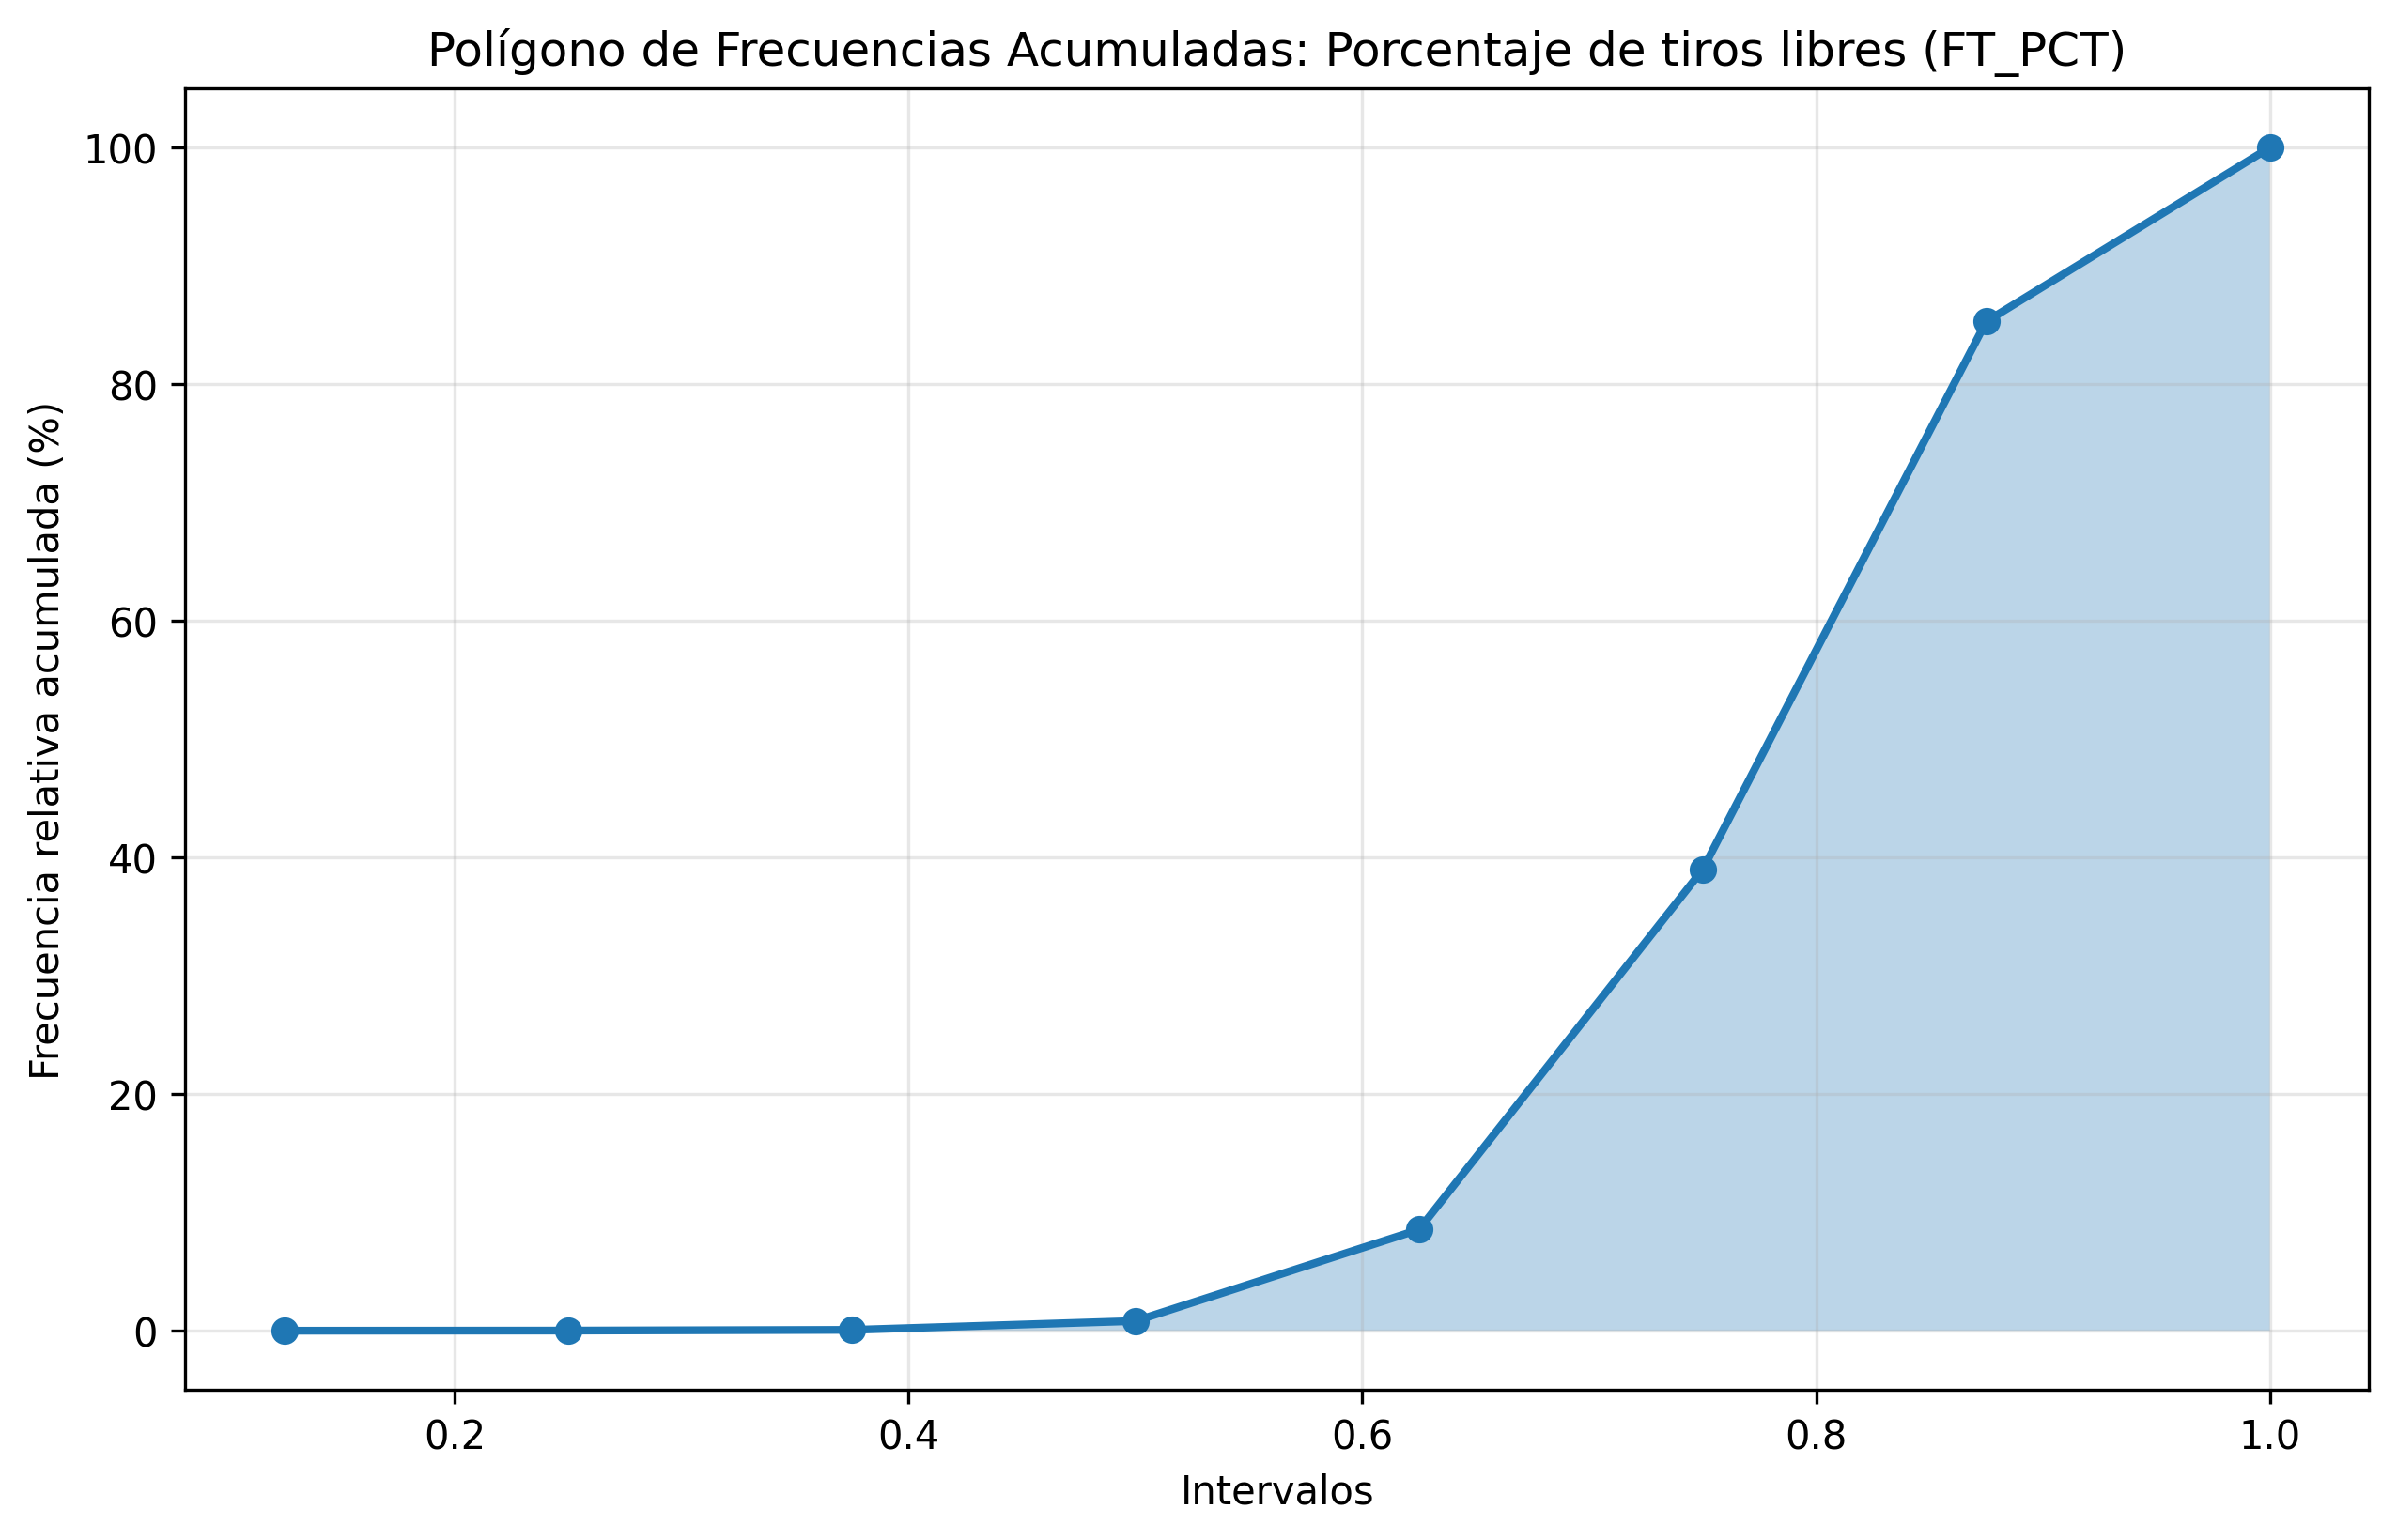
\includegraphics[width=\linewidth]{images/poligono_acumulado_ft_pct.png}
\caption{Polígono acumulado de FT\%}
\label{fig:pol_ft_pct}
\end{minipage}
\end{figure}

El porcentaje de tiros libres presenta una distribución asimétrica con cola hacia la izquierda, centrada en 0.77 (77\%). La coincidencia exacta entre media y mediana ocurre en una distribución no simétrica debido a la compensación entre valores. La concentración principal se observa entre 0.7 y 0.85, indicando que la mayoría de los partidos tienen una eficiencia en tiros libres dentro de este rango. El polígono acumulado muestra una progresión inicial rápida que luego se estabiliza, reflejando que aproximadamente el 80\% de los partidos tienen un porcentaje superior al 70\%.

\subsubsection*{Distribución del Diferencial de Puntos (PLUS\_MINUS)}

\begin{figure}[H]
\centering
\begin{minipage}{0.48\textwidth}
\centering
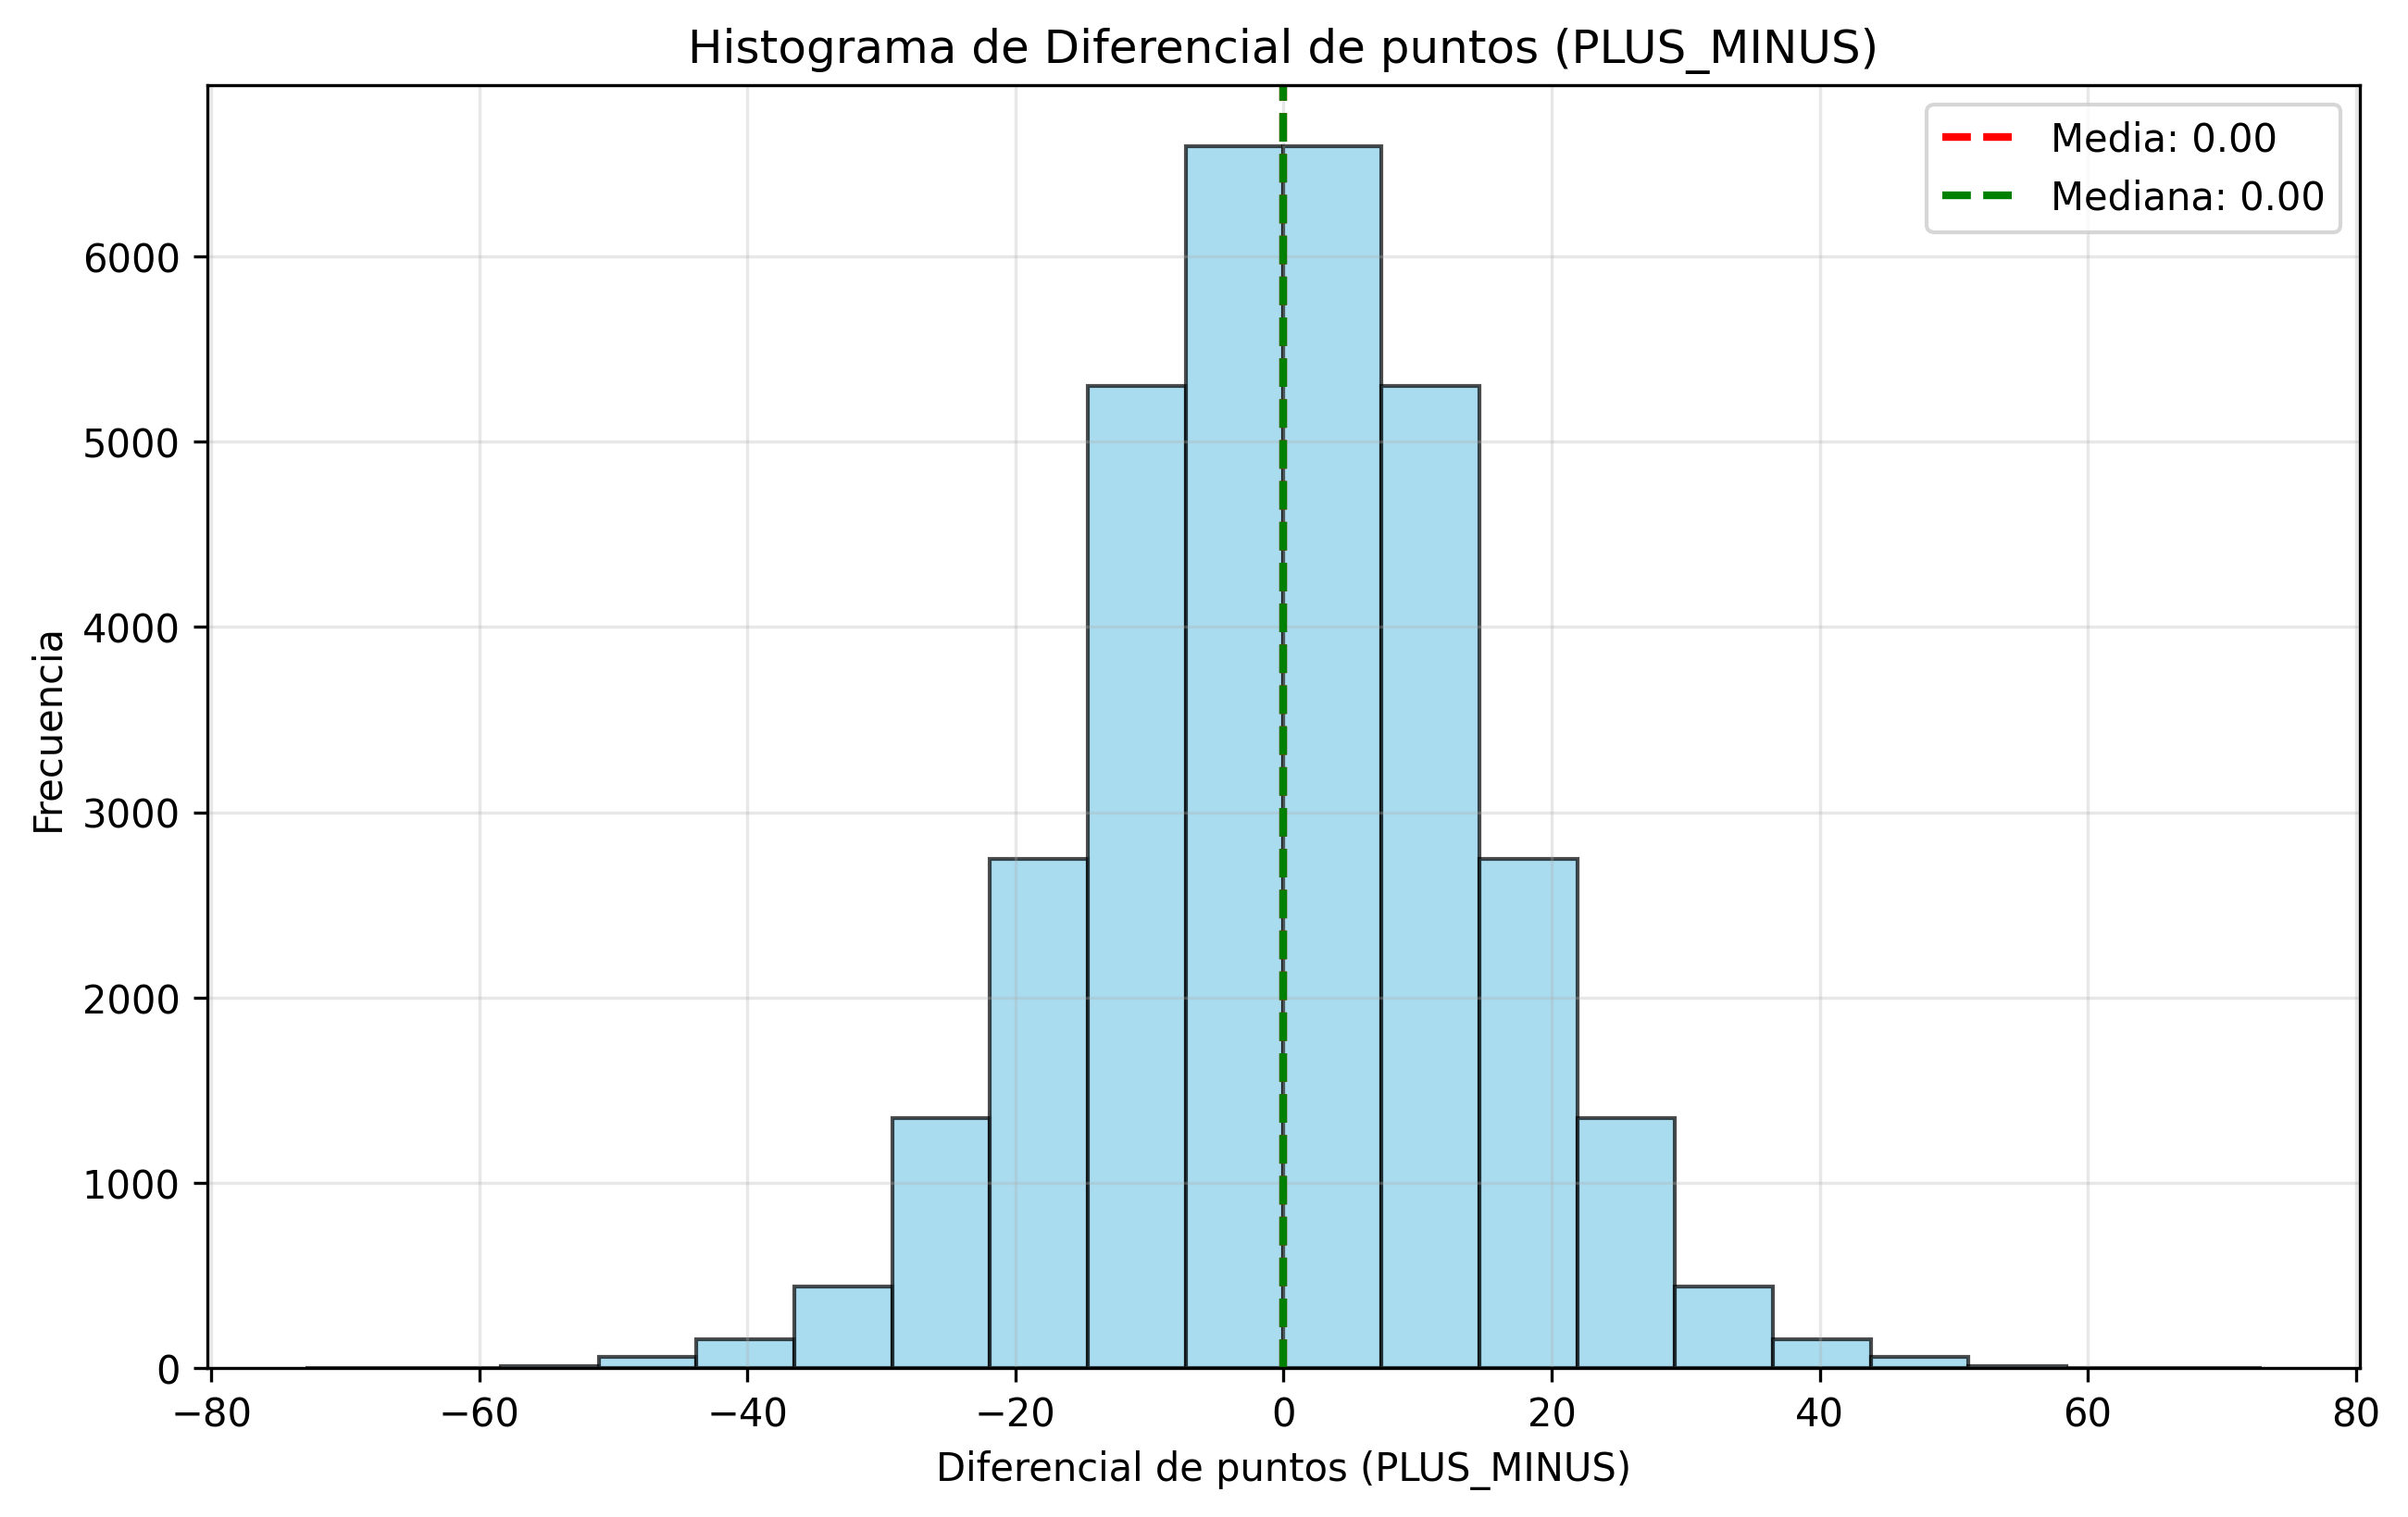
\includegraphics[width=\linewidth]{images/histograma_plus_minus.png}
\caption{Histograma de Diferencial de Puntos (PLUS\_MINUS). Media: 0.00, Mediana: 0.00}
\label{fig:hist_plus_minus}
\end{minipage}
\hfill
\begin{minipage}{0.48\textwidth}
\centering
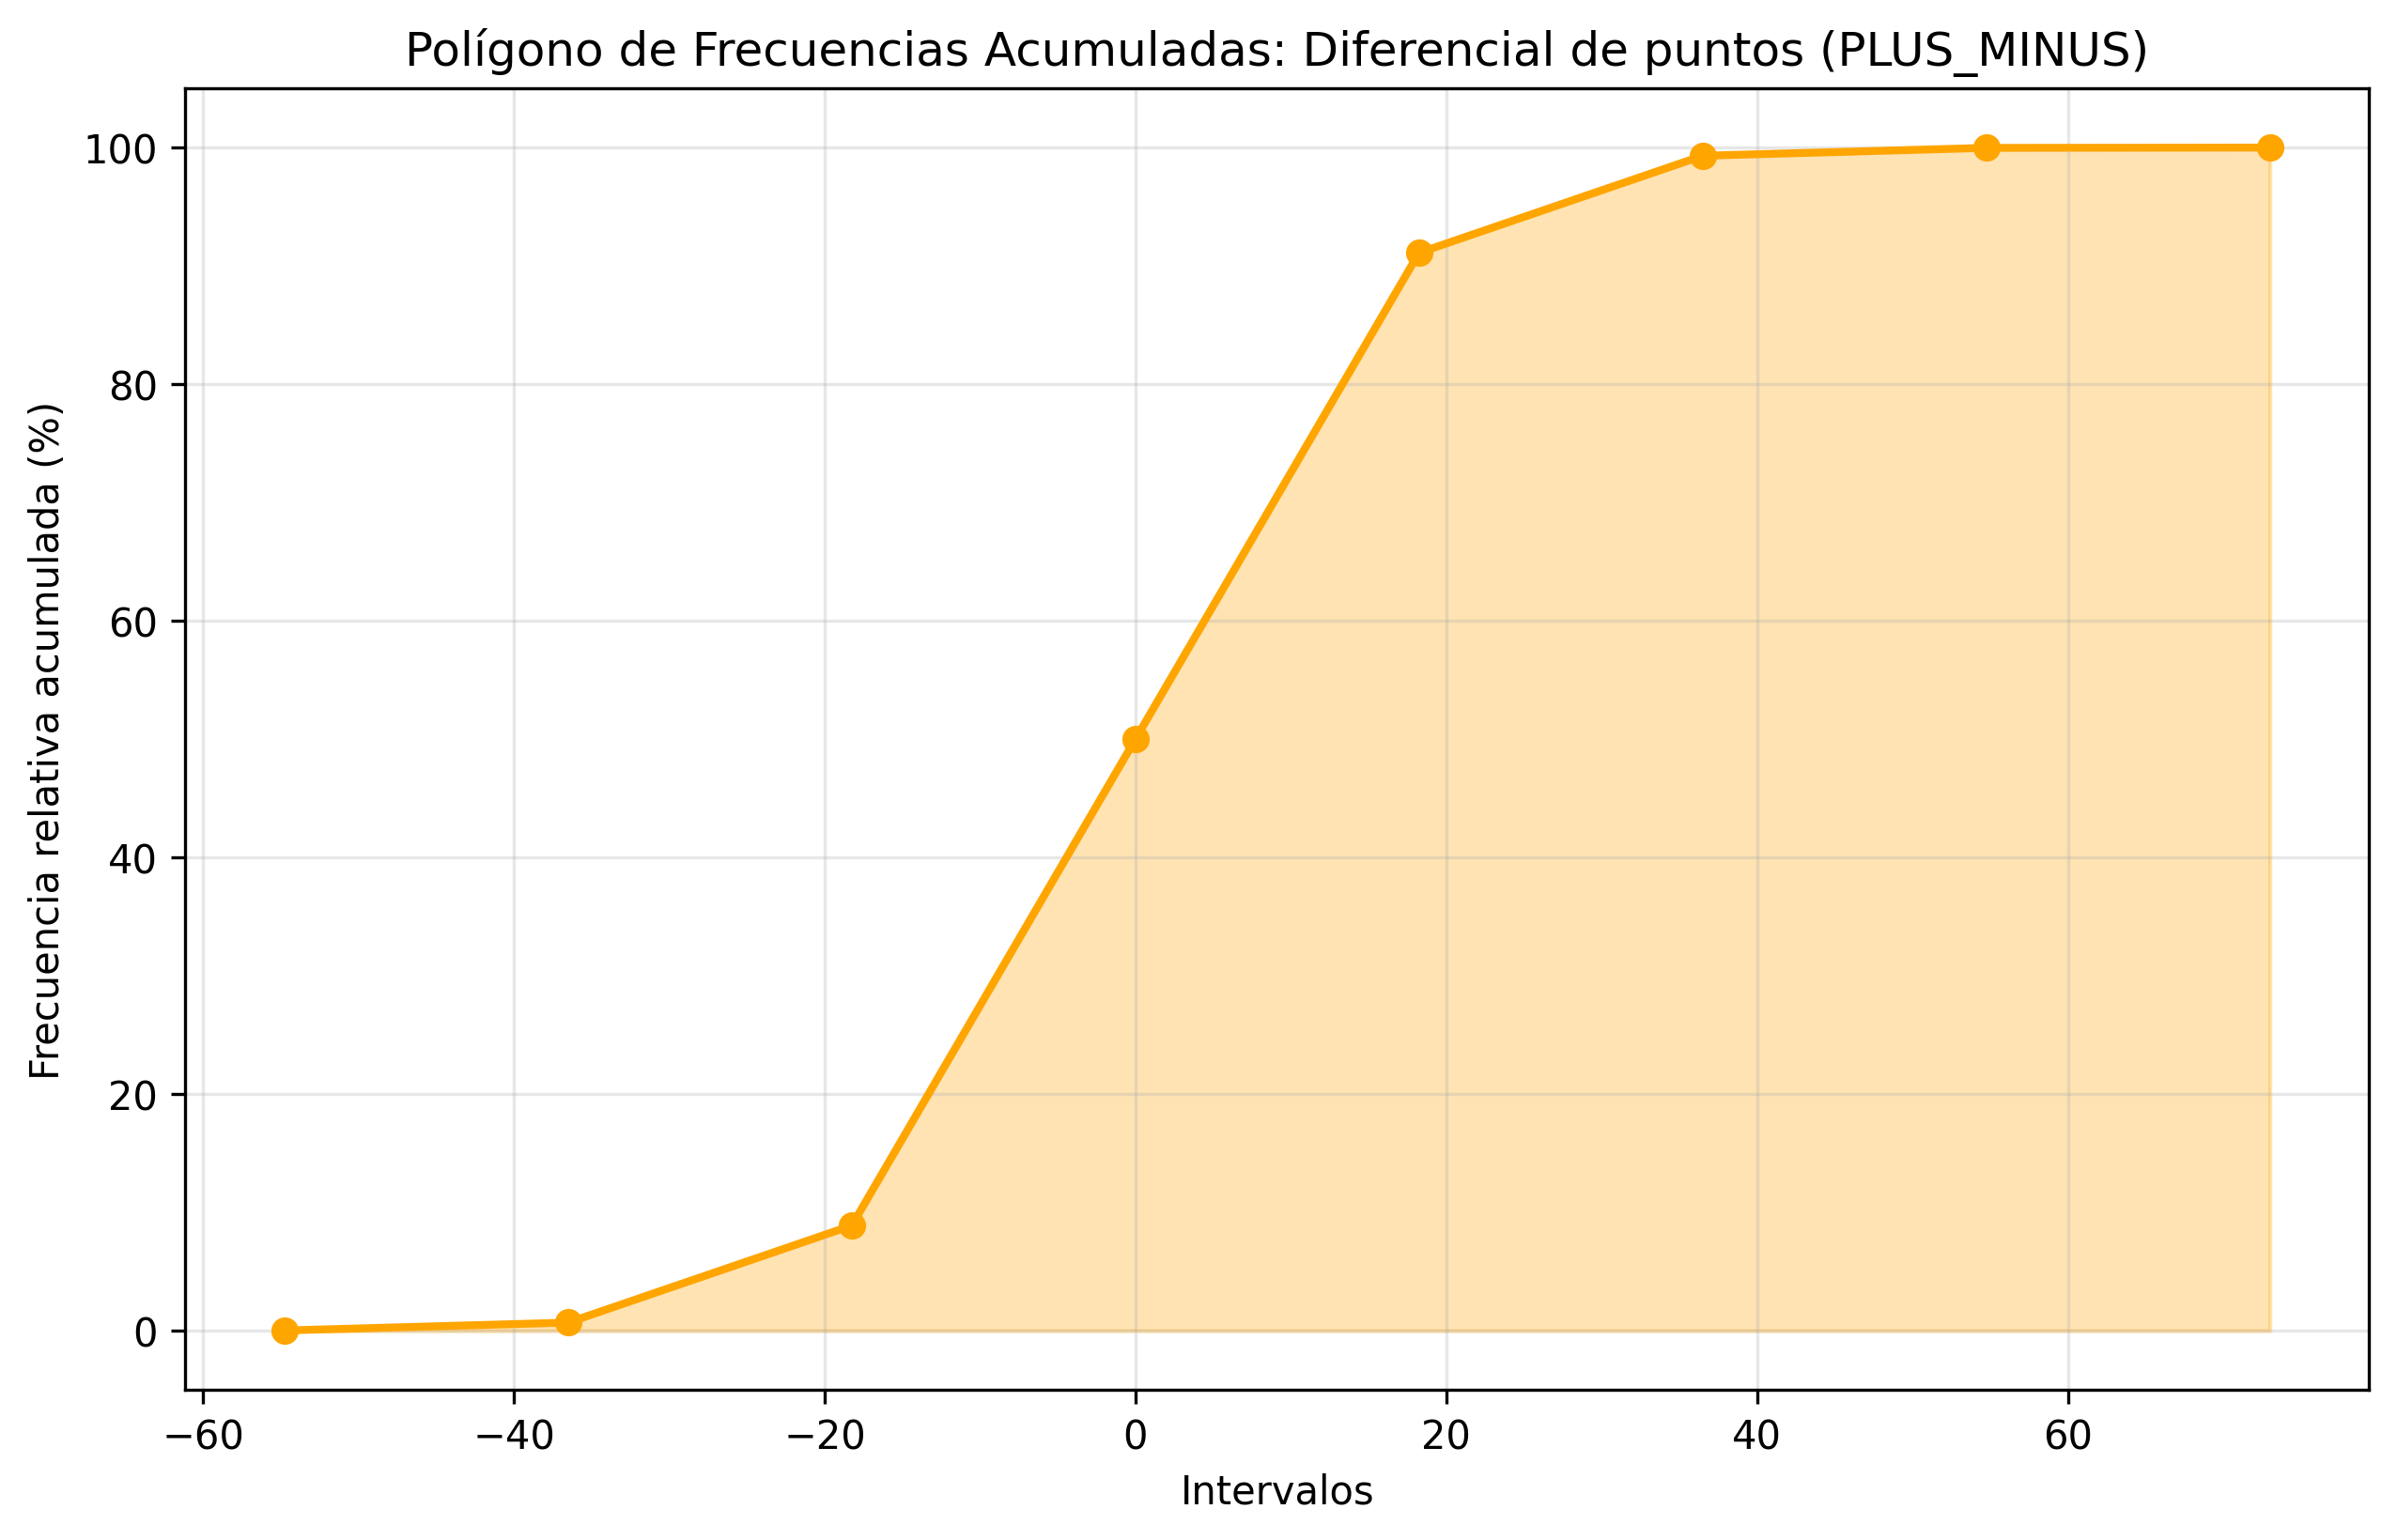
\includegraphics[width=\linewidth]{images/poligono_acumulado_plus_minus.png}
\caption{Polígono acumulado de PLUS\_MINUS}
\label{fig:pol_plus_minus}
\end{minipage}
\end{figure}

El diferencial de puntos muestra una distribución perfectamente simétrica centrada en cero, como era de esperar en un conjunto de datos balanceado que incluye tanto victorias como derrotas. La forma aproximadamente normal con colas extendidas indica la presencia de partidos con diferencias extremas en ambas direcciones. La coincidencia exacta entre media y mediana en cero confirma el perfecto equilibrio de la distribución. El polígono acumulado presenta la clásica forma de S invertida, con punto de inflexión exactamente en el 50\%, indicando que la mitad de los partidos tienen diferencial negativo y la otra mitad positivo.

\subsubsection*{Distribución de Robos de Balón (STL)}

\begin{figure}[H]
\centering
\begin{minipage}{0.48\textwidth}
\centering
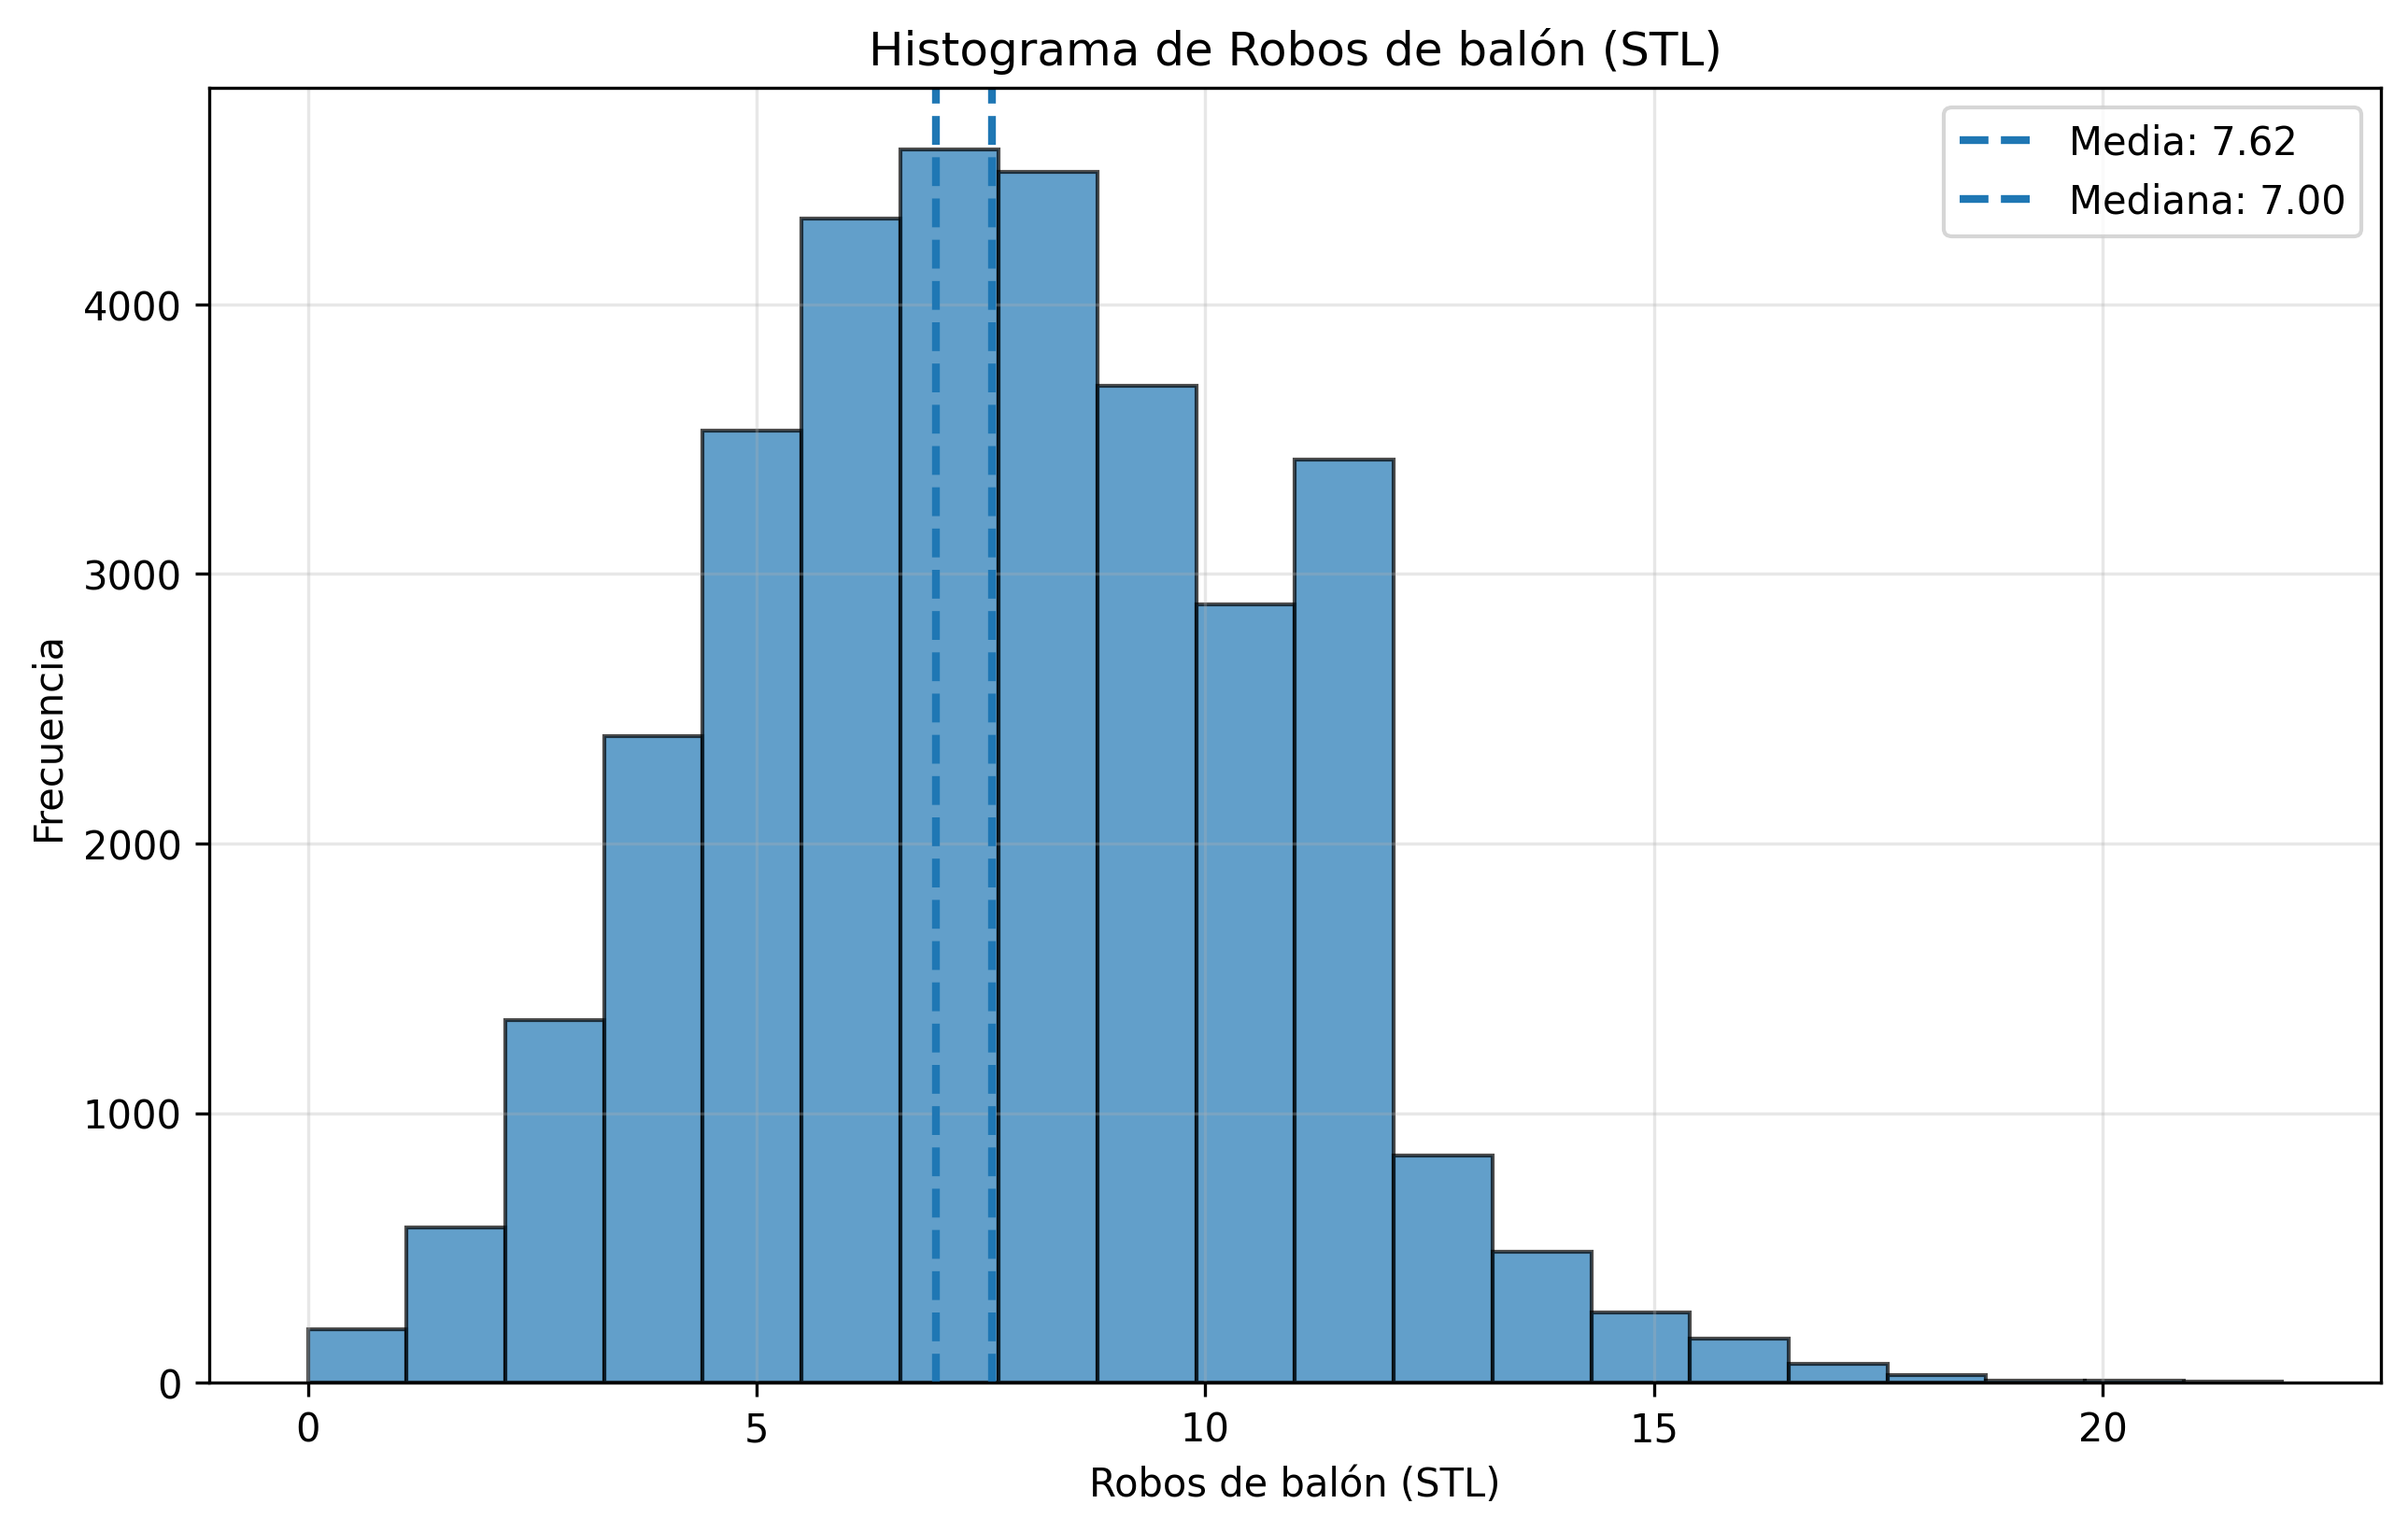
\includegraphics[width=\linewidth]{images/histograma_stl.png}
\caption{Histograma de Robos de Balón (STL). Media: 7.62, Mediana: 7.00}
\label{fig:hist_stl}
\end{minipage}
\hfill
\begin{minipage}{0.48\textwidth}
\centering
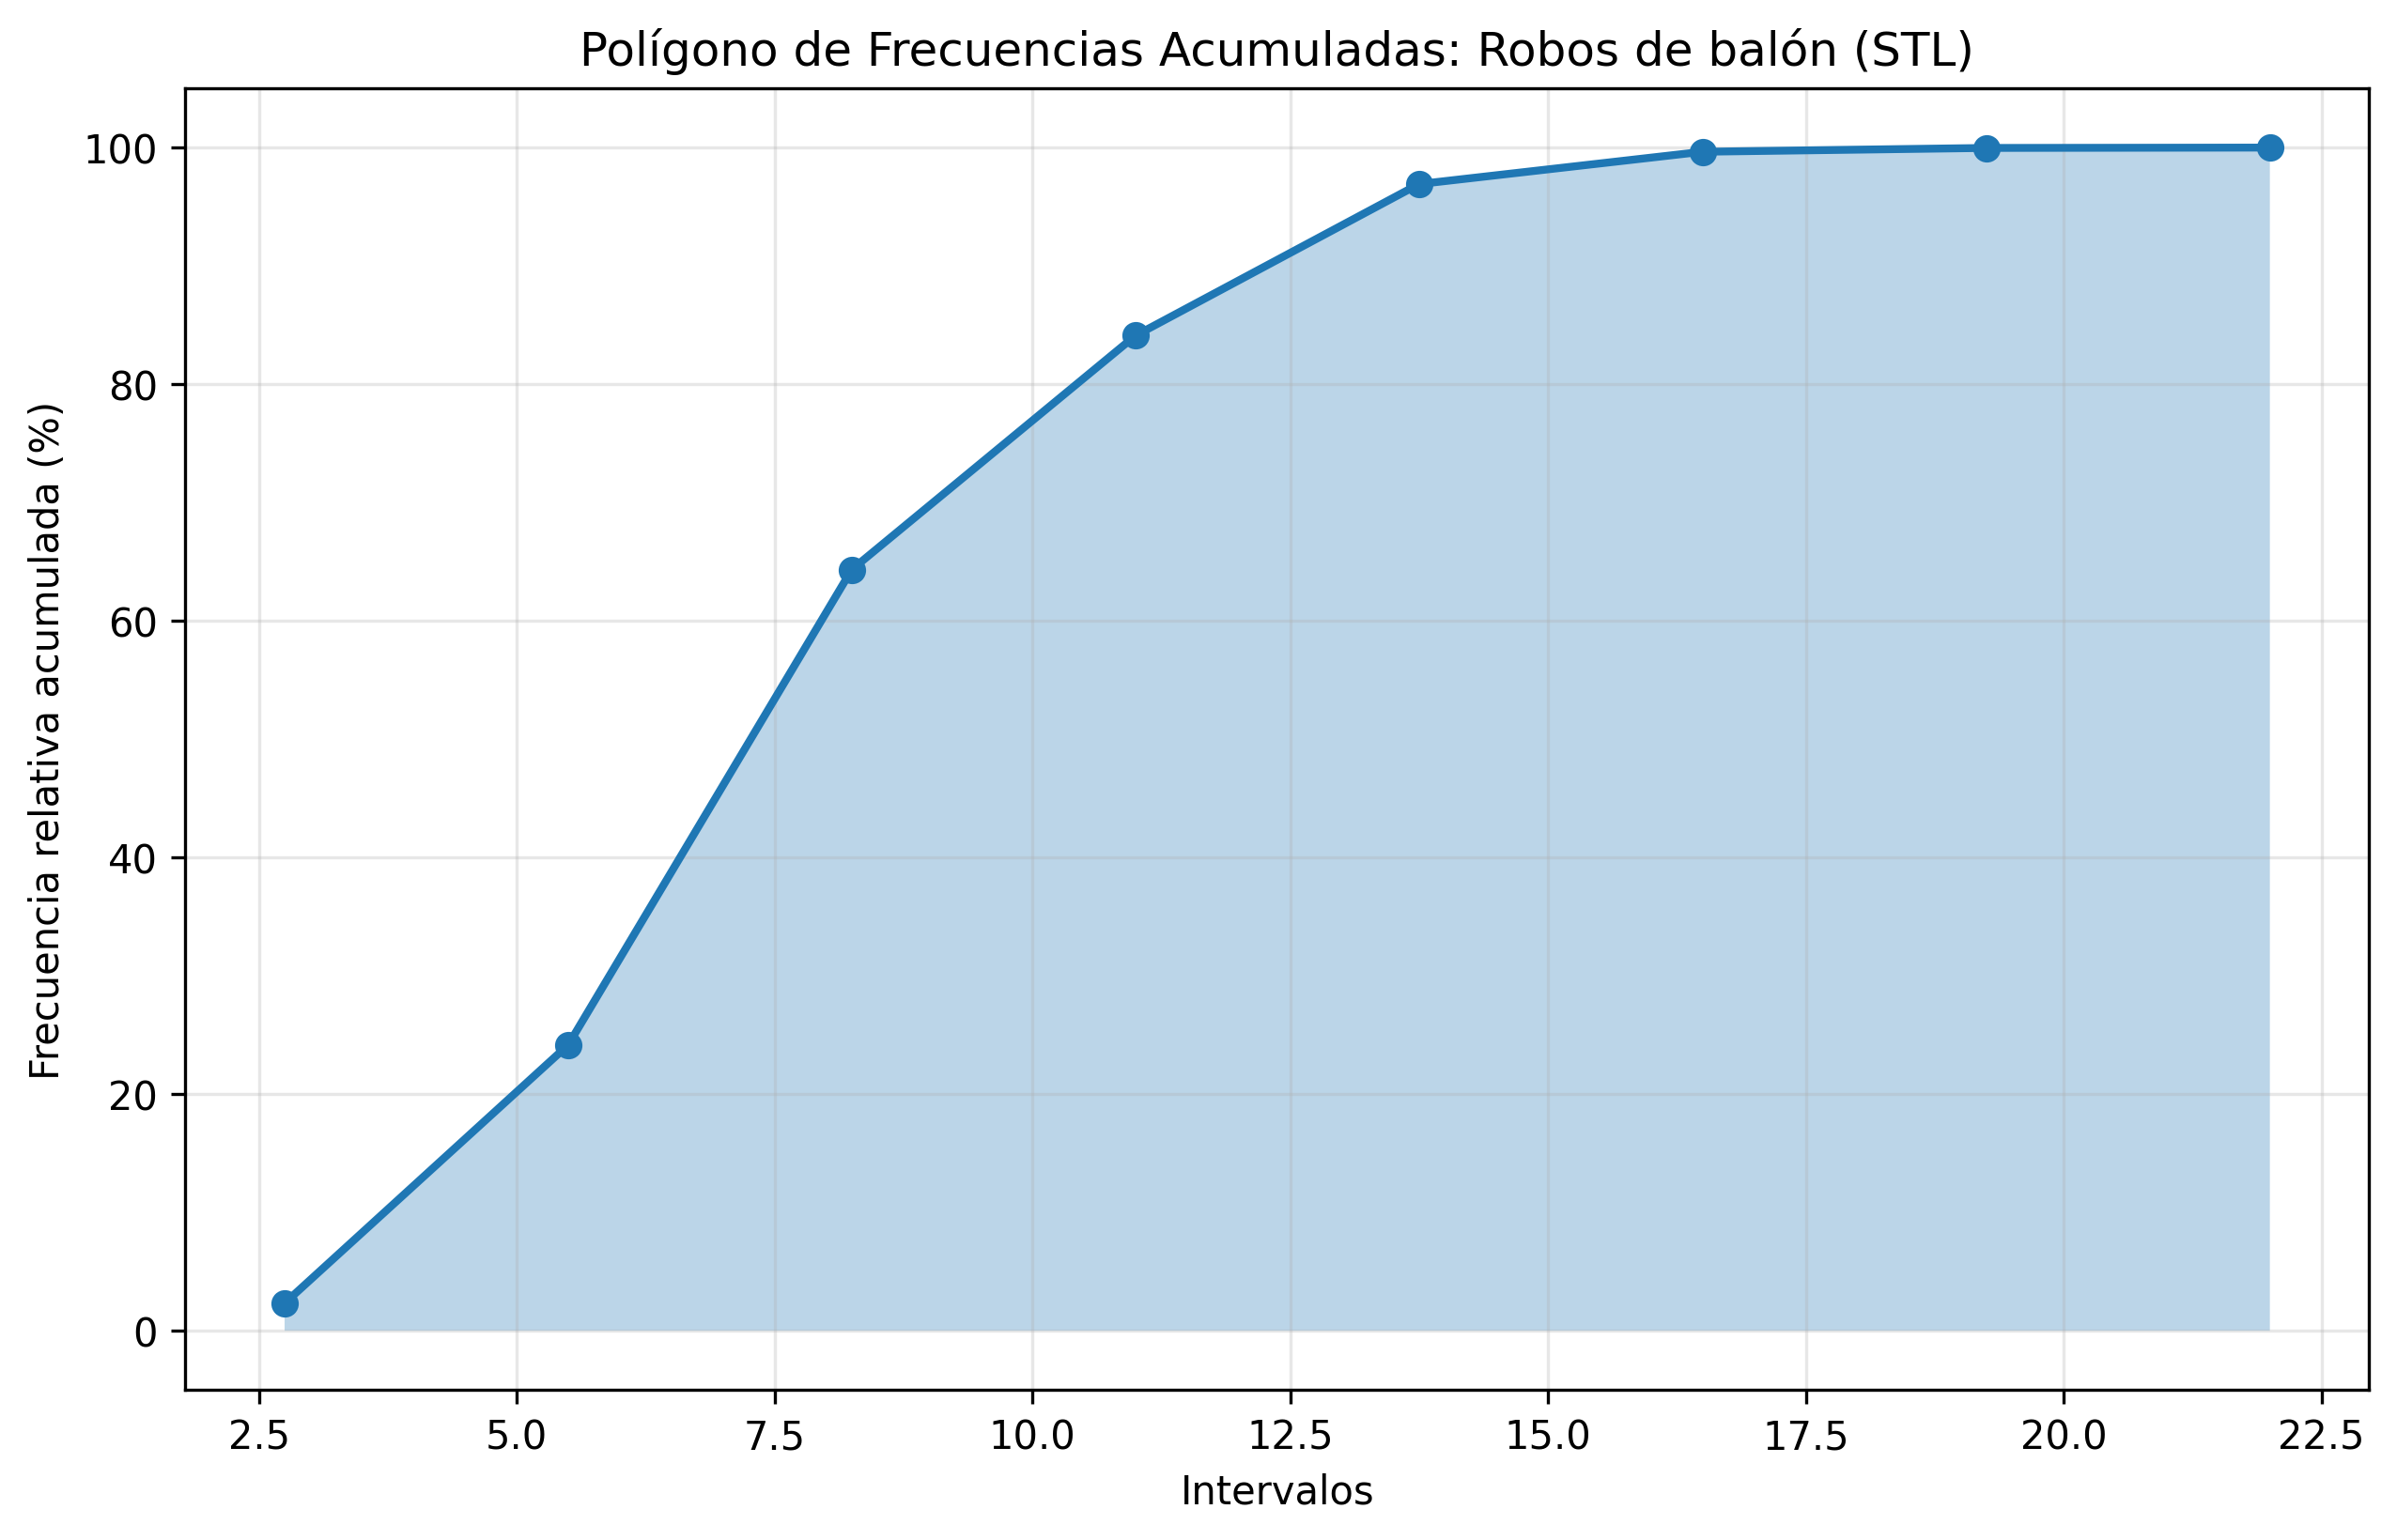
\includegraphics[width=\linewidth]{images/poligono_acumulado_stl.png}
\caption{Polígono acumulado de STL}
\label{fig:pol_stl}
\end{minipage}
\end{figure}

Los robos de balón muestran una distribución claramente asimétrica con cola hacia la derecha, típica de variables con límite inferior en cero. La diferencia entre media (7.62) y mediana (7.00) confirma esta asimetría. La mayoría de los partidos registran entre 5 y 10 robos, con una frecuencia que disminuye rápidamente para valores superiores. El polígono acumulado muestra una curva de crecimiento rápido inicial que luego se suaviza, indicando que aproximadamente el 80\% de los partidos tienen menos de 10 robos.

\subsubsection*{Distribución de Bloques (BLK)}

\begin{figure}[H]
\centering
\begin{minipage}{0.48\textwidth}
\centering
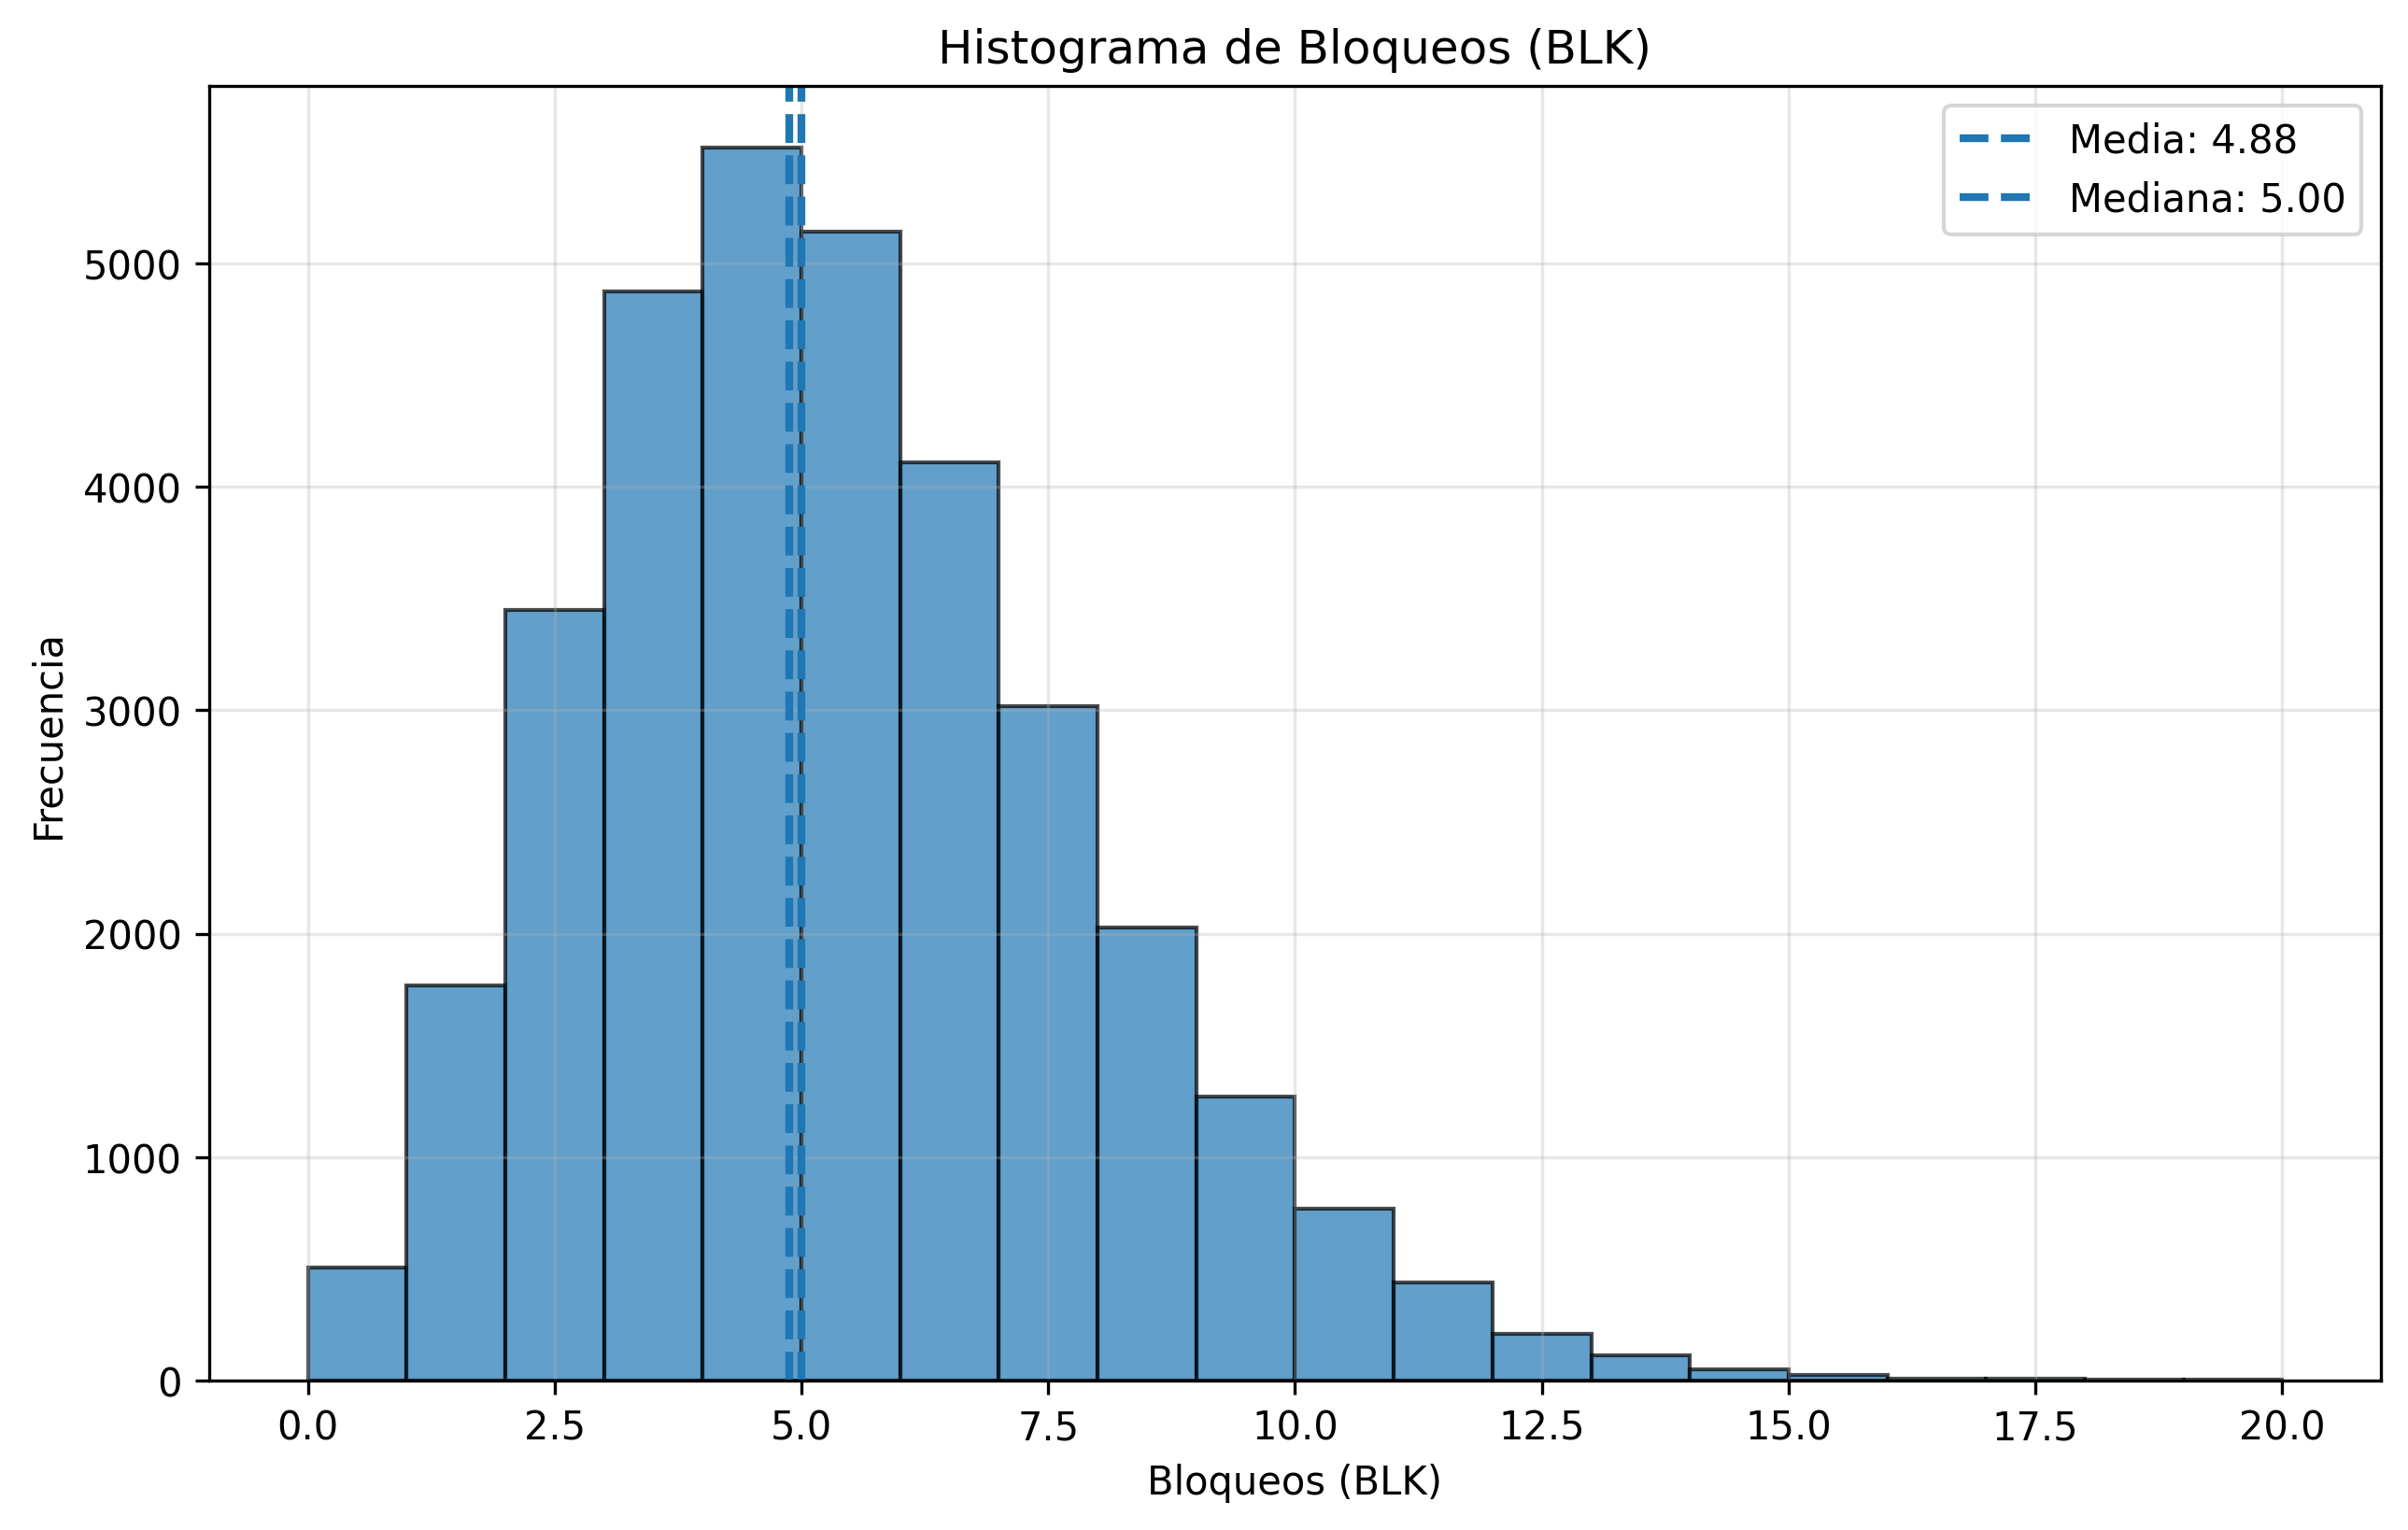
\includegraphics[width=\linewidth]{images/histograma_blk.png}
\caption{Histograma de Bloques (BLK). Media: 4.88, Mediana: 5.00}
\label{fig:hist_blk}
\end{minipage}
\hfill
\begin{minipage}{0.48\textwidth}
\centering
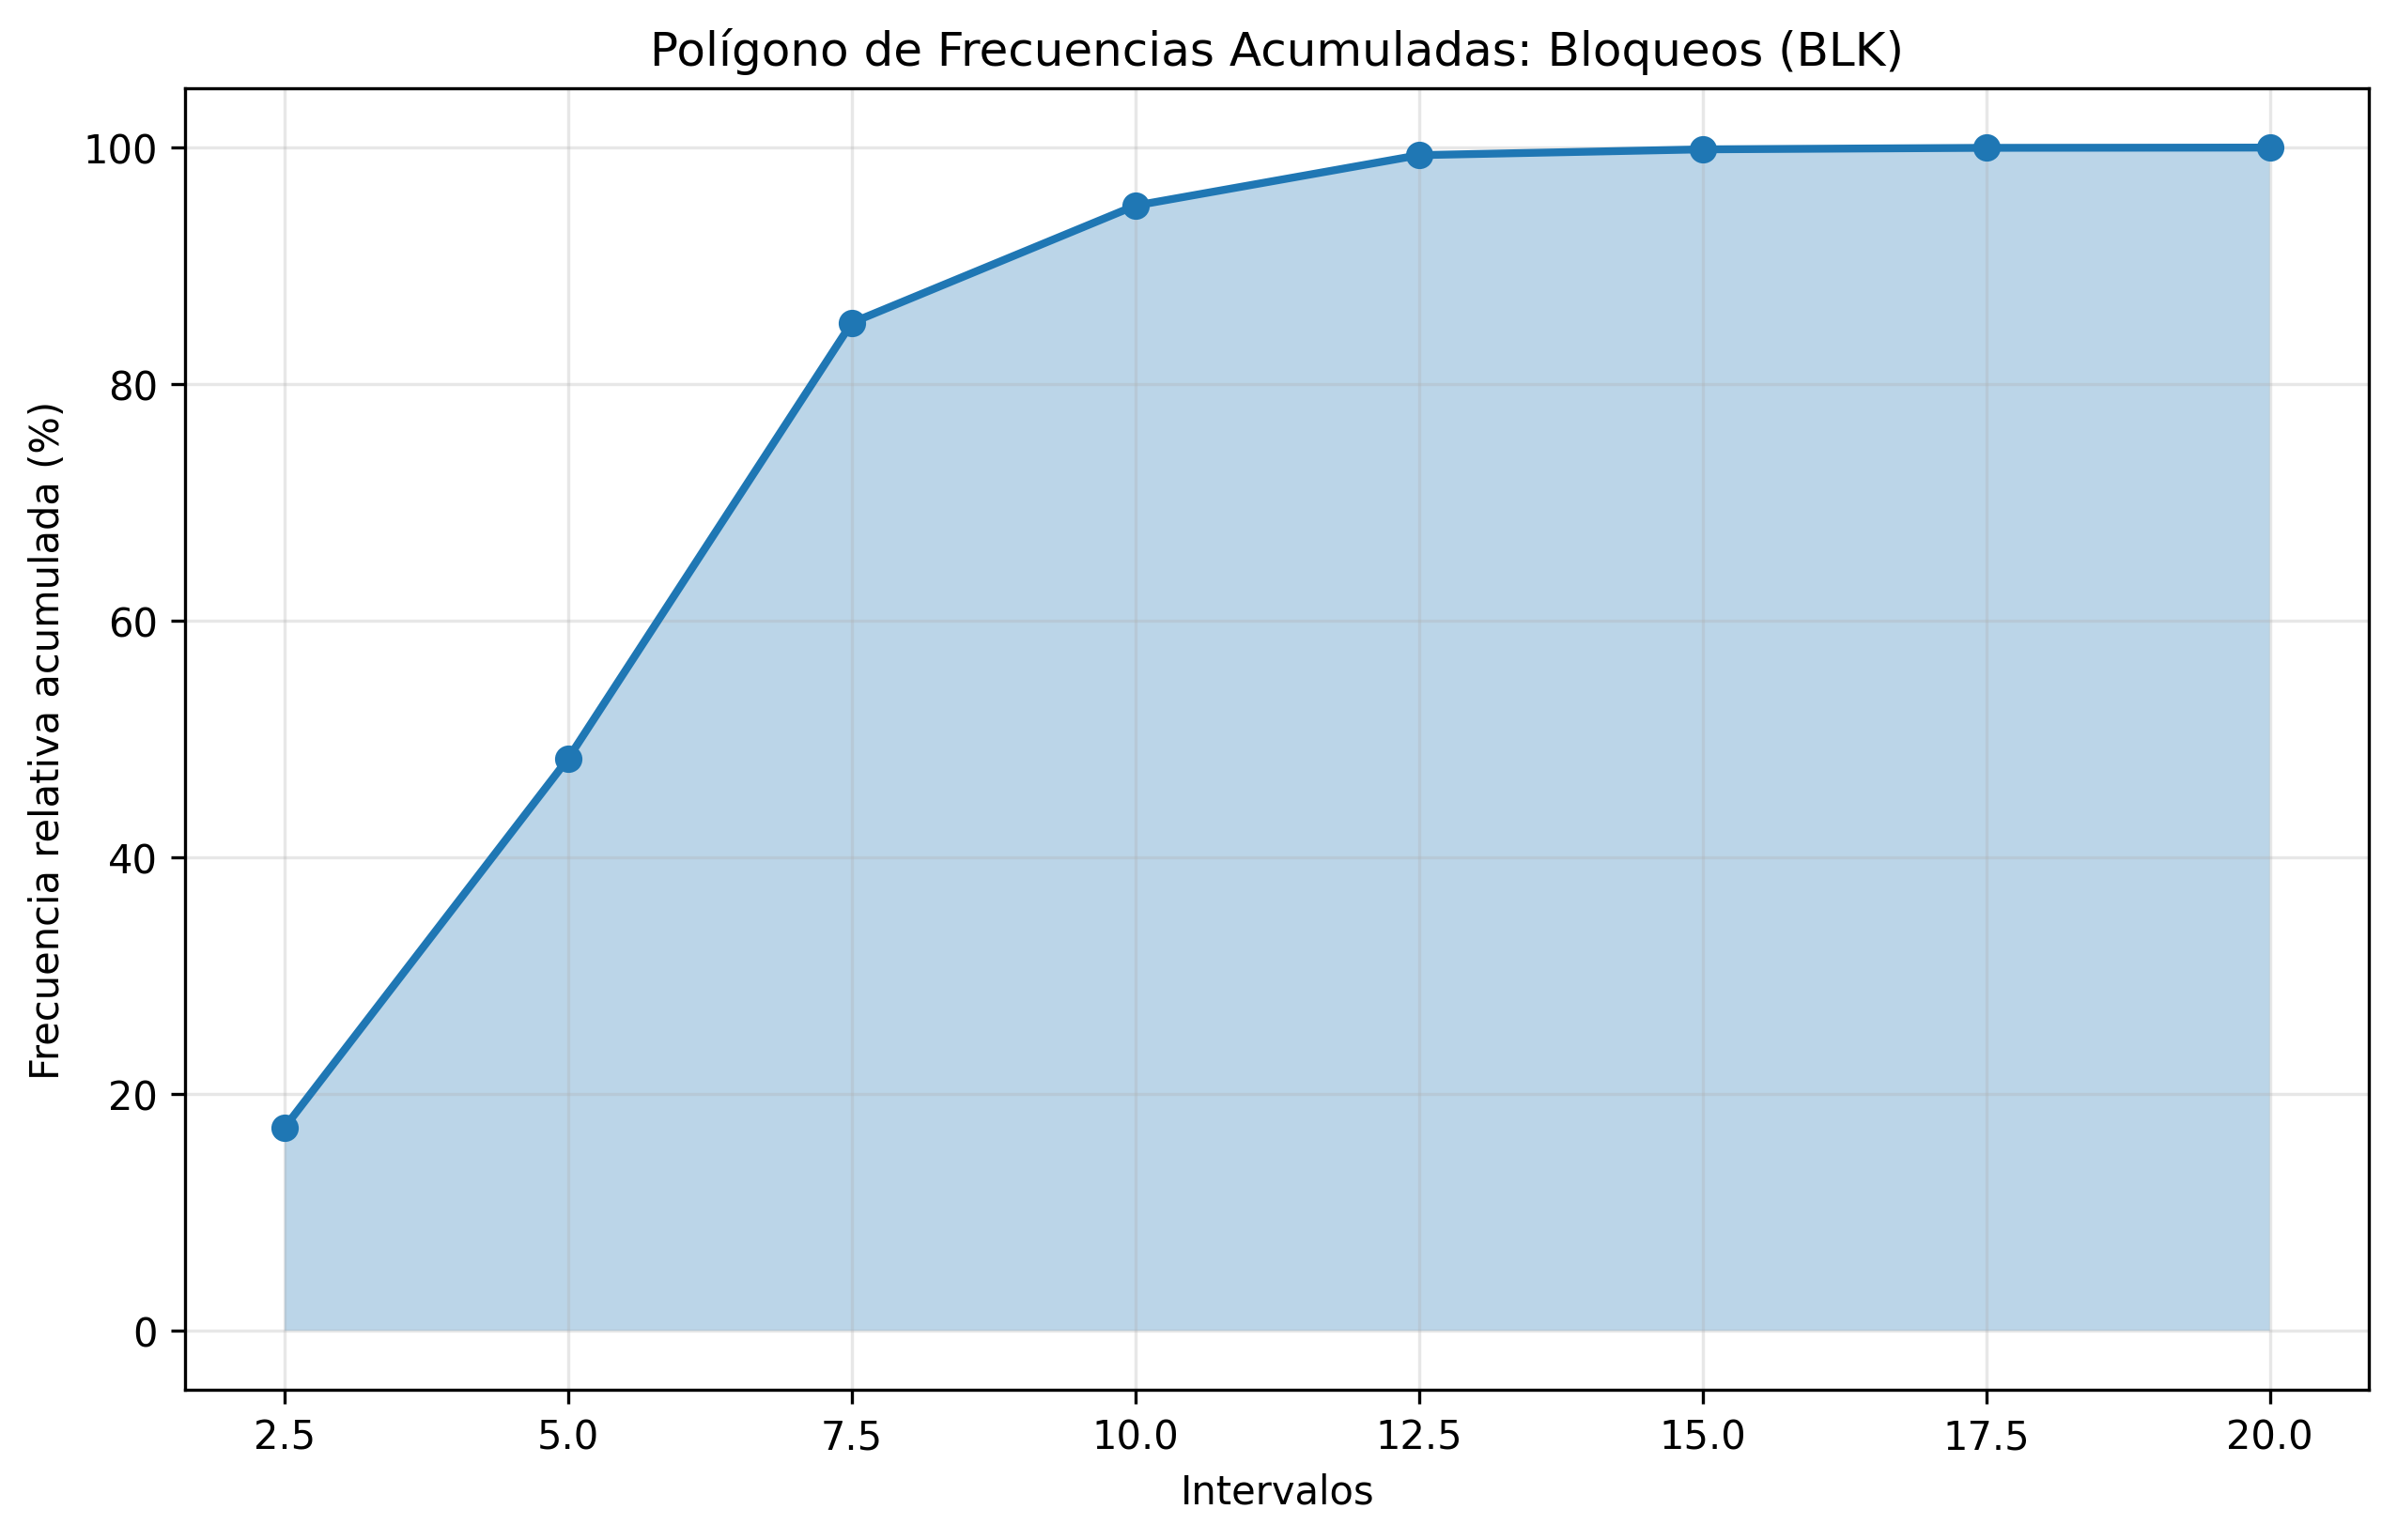
\includegraphics[width=\linewidth]{images/poligono_acumulado_blk.png}
\caption{Polígono acumulado de Bloques (BLK)}
\label{fig:pol_blk}
\end{minipage}
\end{figure}

La distribución de bloques por partido muestra una asimetría marcada hacia la derecha, típica de variables con límite inferior en cero. La mayoría de los partidos registran entre 2.5 y 7.5 bloques, con un pico alrededor de 5 bloques. La proximidad entre media (4.88) y mediana (5.00) sugiere una distribución razonablemente equilibrada pese a la asimetría. El polígono acumulado presenta una curva de crecimiento rápido inicial que luego se suaviza, indicando que aproximadamente el 80\% de los partidos tienen menos de 10 bloques.

\subsubsection*{Distribución de la Proporción de Triples Intentados (FG3A/FGA)}

\begin{figure}[H]
\centering
\begin{minipage}{0.48\textwidth}
\centering
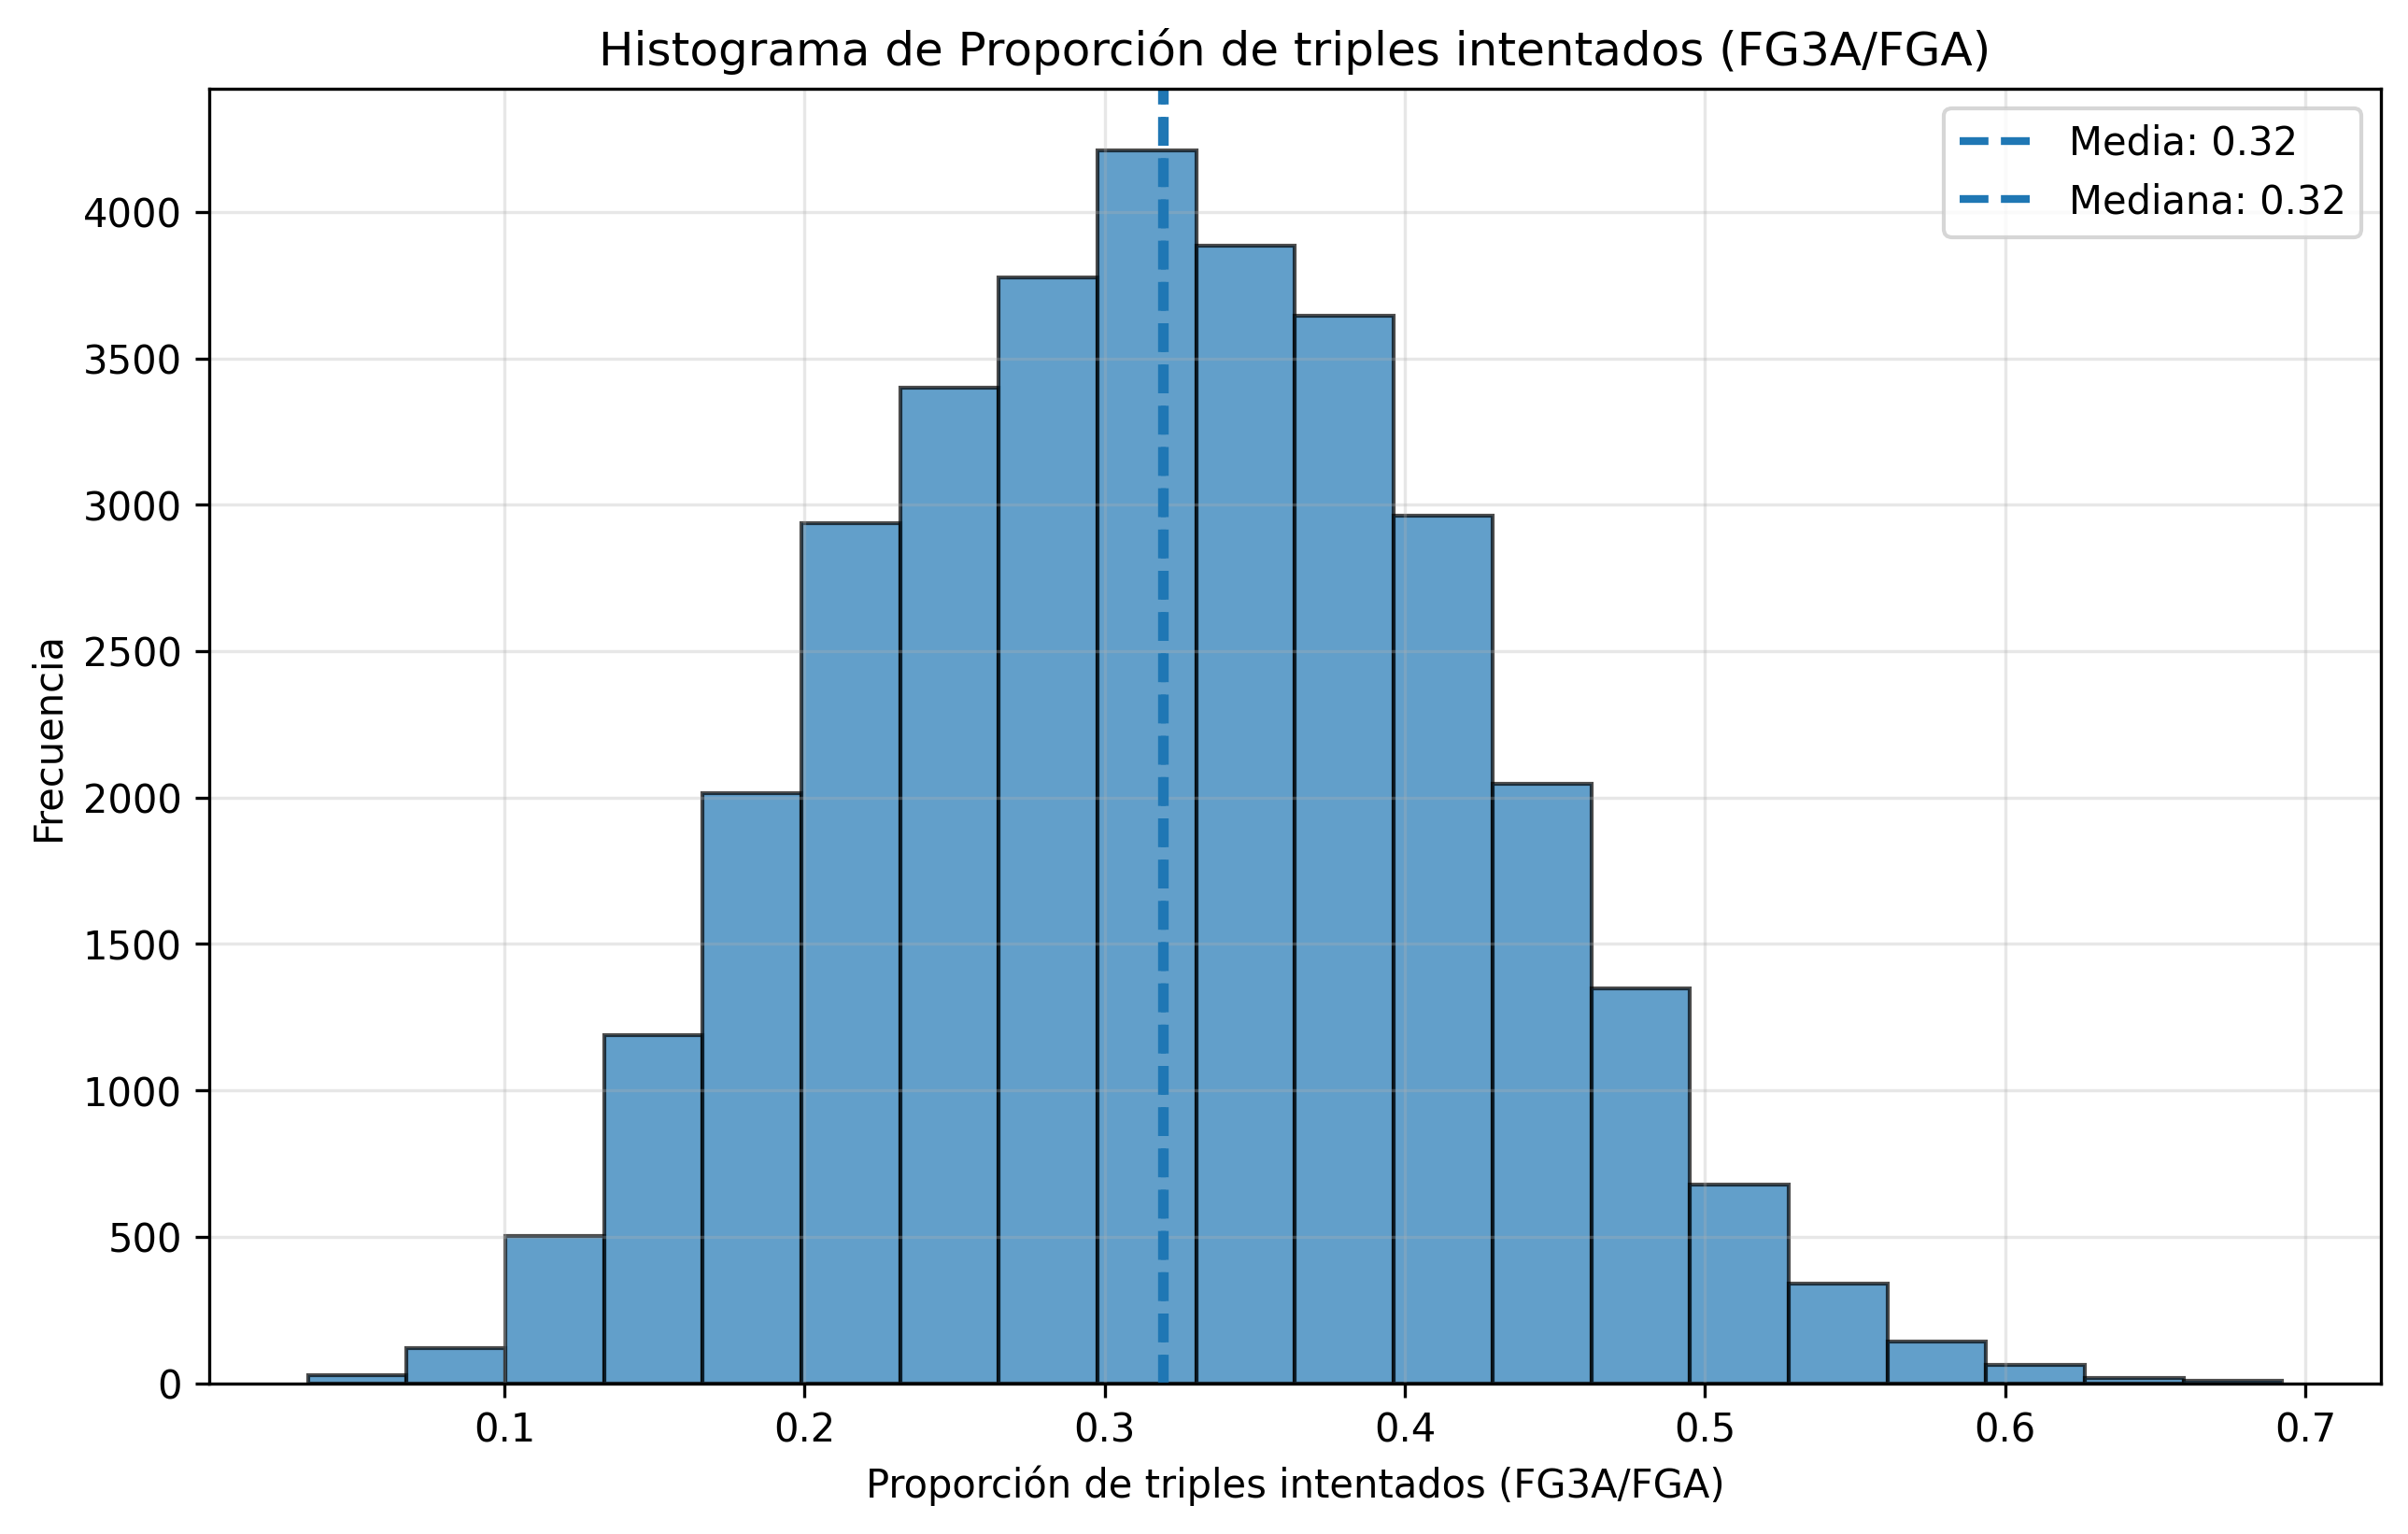
\includegraphics[width=\linewidth]{images/histograma_fg3a_fga.png}
\caption{Histograma de Proporción FG3A/FGA. Media: 0.32, Mediana: 0.32}
\label{fig:hist_fg3a_fga}
\end{minipage}
\hfill
\begin{minipage}{0.48\textwidth}
\centering
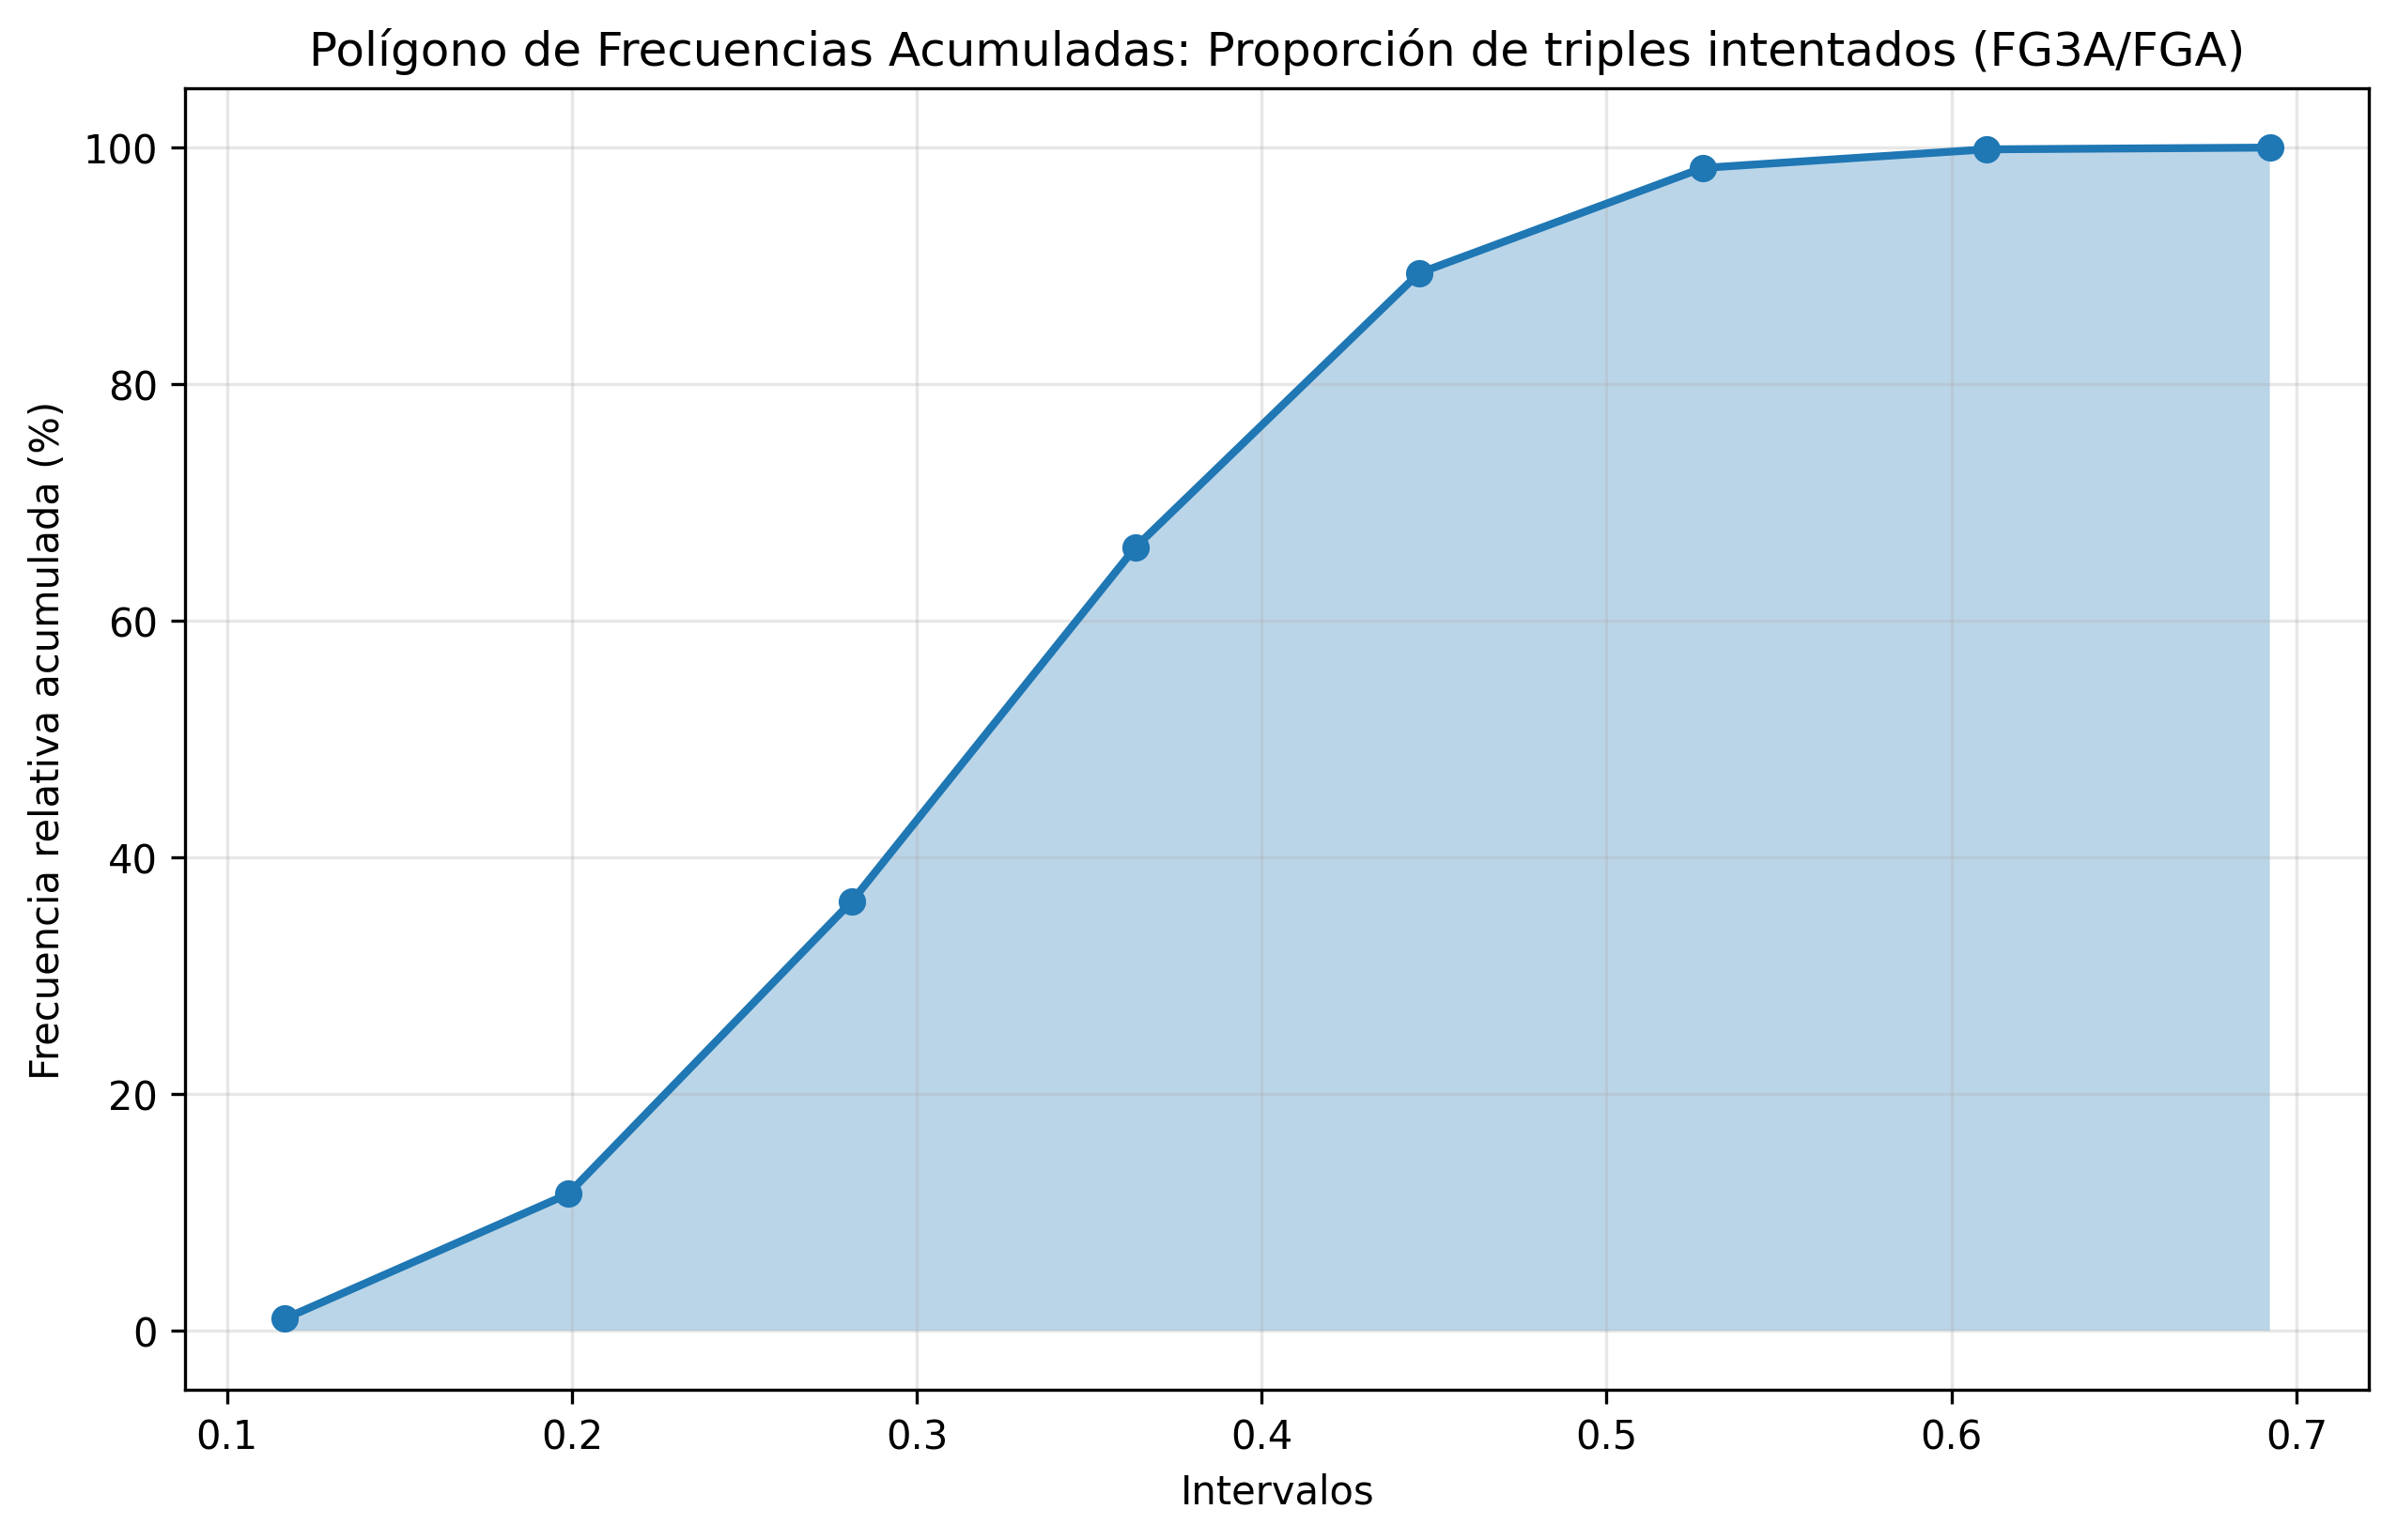
\includegraphics[width=\linewidth]{images/poligono_acumulado_fg3a_fga.png}
\caption{Polígono acumulado de FG3A/FGA}
\label{fig:pol_fg3a_fga}
\end{minipage}
\end{figure}

La proporción de triples intentados respecto al total de tiros muestra una distribución aproximadamente normal centrada en 0.32 (32\%), con coincidencia exacta entre media y mediana. Esto indica que, en promedio, aproximadamente un tercio de los tiros de campo son intentos de tres puntos. La distribución compacta alrededor de este valor sugiere una relativa homogeneidad en las estrategias ofensivas entre equipos y partidos. El polígono acumulado muestra una curva suave y simétrica, confirmando la consistencia en esta proporción, con aproximadamente el 50\% de los partidos registrando una proporción inferior al 32\%.

\subsection{Boxplots y Detección de Valores Atípicos}
\label{subsec:boxplots}

Con el objetivo de complementar el análisis descriptivo previo basado en histogramas y
polígonos acumulados, se emplean boxplots para examinar la dispersión, simetría y presencia
de valores atípicos en las variables cuantitativas seleccionadas. Este tipo de representación
permite identificar de manera sintética la estructura central de los datos mediante la mediana,
el rango intercuartílico y los extremos no atípicos, así como detectar observaciones extremas
que pueden resultar relevantes en el contexto competitivo o para la especificación de modelos
estadísticos posteriores.

\subsubsection*{Resumen del grupo: métricas de volumen, tiro exterior y control del juego}

Las variables incluidas en este grupo (\textit{PTS, FG3M, FG3A, AST, REB y TOV}) representan métricas
de \textbf{volumen ofensivo, generación colectiva, orientación al tiro exterior y control del ritmo
de juego}. En conjunto, los boxplots muestran distribuciones mayormente simétricas, con medias y
medianas próximas, lo que sugiere un comportamiento estable de estas variables a lo largo del
conjunto de partidos analizados. Los rangos intercuartílicos son moderados en todas las métricas,
indicando que, si bien existe variabilidad natural entre encuentros, el desempeño del equipo se
concentra alrededor de valores centrales bien definidos.

Un rasgo común del grupo es la presencia de \textbf{valores atípicos en ambos extremos}, asociados a
partidos con condiciones excepcionales, como ritmos de juego inusualmente altos o bajos,
diferencias marcadas en el nivel de los oponentes o ajustes tácticos específicos. Estos valores no
alteran la estructura central de las distribuciones, pero aportan información relevante sobre
escenarios de desempeño extremo.

Desde una perspectiva comparativa, cada variable resalta un aspecto particular del juego.
\textit{PTS} sintetiza el resultado final de la producción ofensiva total; \textit{AST} refleja el
grado de juego colectivo y la circulación del balón; \textit{REB} captura el control físico y
posicional del partido; \textit{TOV} actúa como un indicador inverso del orden y la eficiencia en la
ejecución ofensiva. En relación con el tiro exterior, \textit{FG3A} evidencia la orientación táctica
hacia el lanzamiento de tres puntos, mientras que \textit{FG3M} muestra una mayor dispersión,
confirmando el carácter situacional y dependiente del acierto de esta variable dentro del juego.

En conjunto, estas métricas ofrecen una visión coherente y complementaria del estilo de juego del
equipo. Por esta razón, se presenta únicamente una selección representativa de boxplots, evitando
redundancias descriptivas sin pérdida de información analítica relevante.

\begin{figure}[H]
    \centering
    \begin{subfigure}[b]{0.3\textwidth}
        \centering
        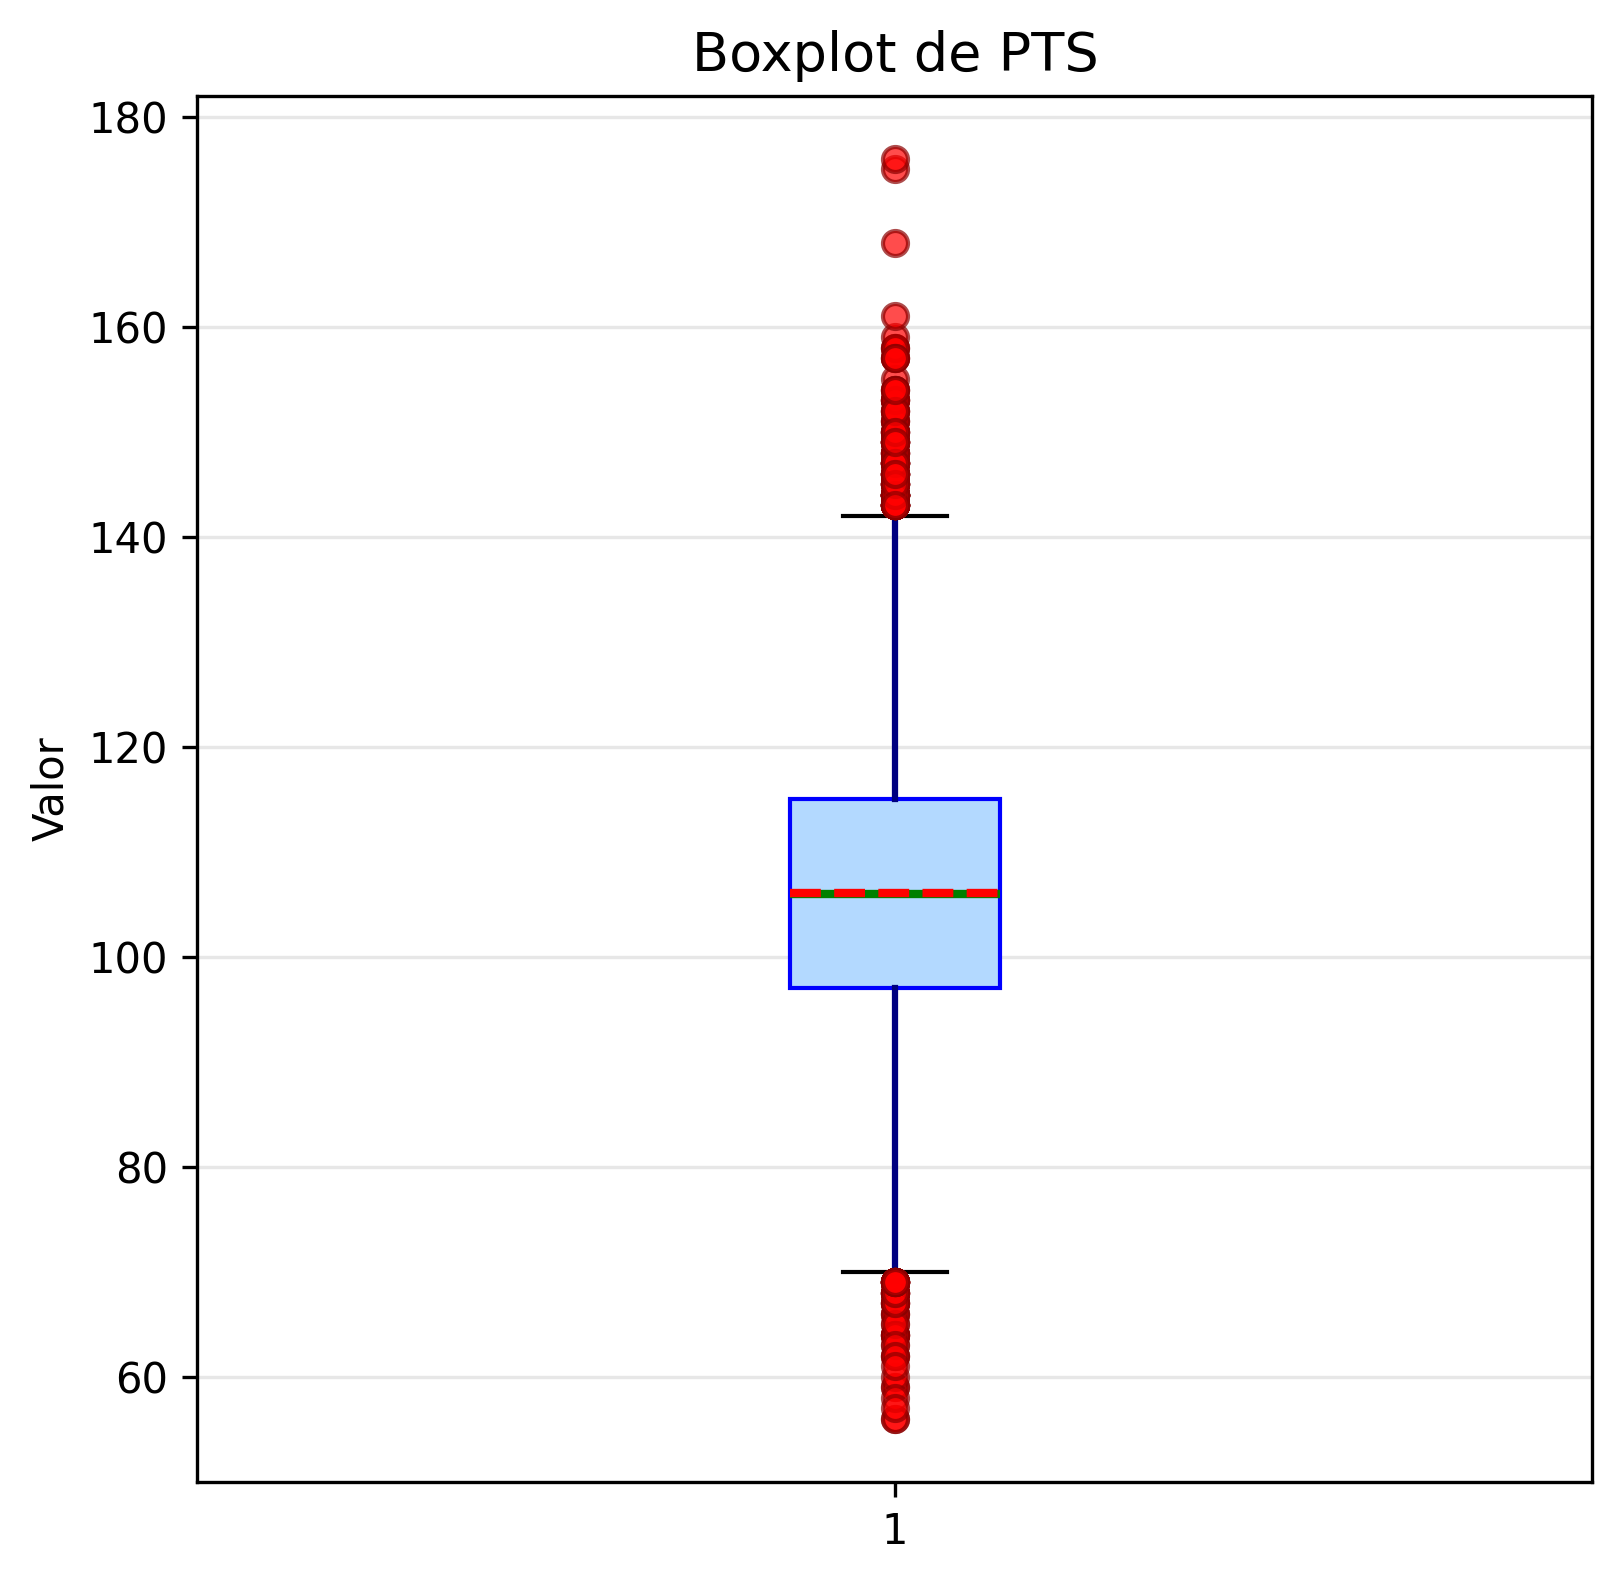
\includegraphics[width=\textwidth]{images/boxplots/boxplot_PTS.png}
        \caption{PTS}
        \label{fig:PTS}
    \end{subfigure}
    \hfill
    \begin{subfigure}[b]{0.3\textwidth}
        \centering
        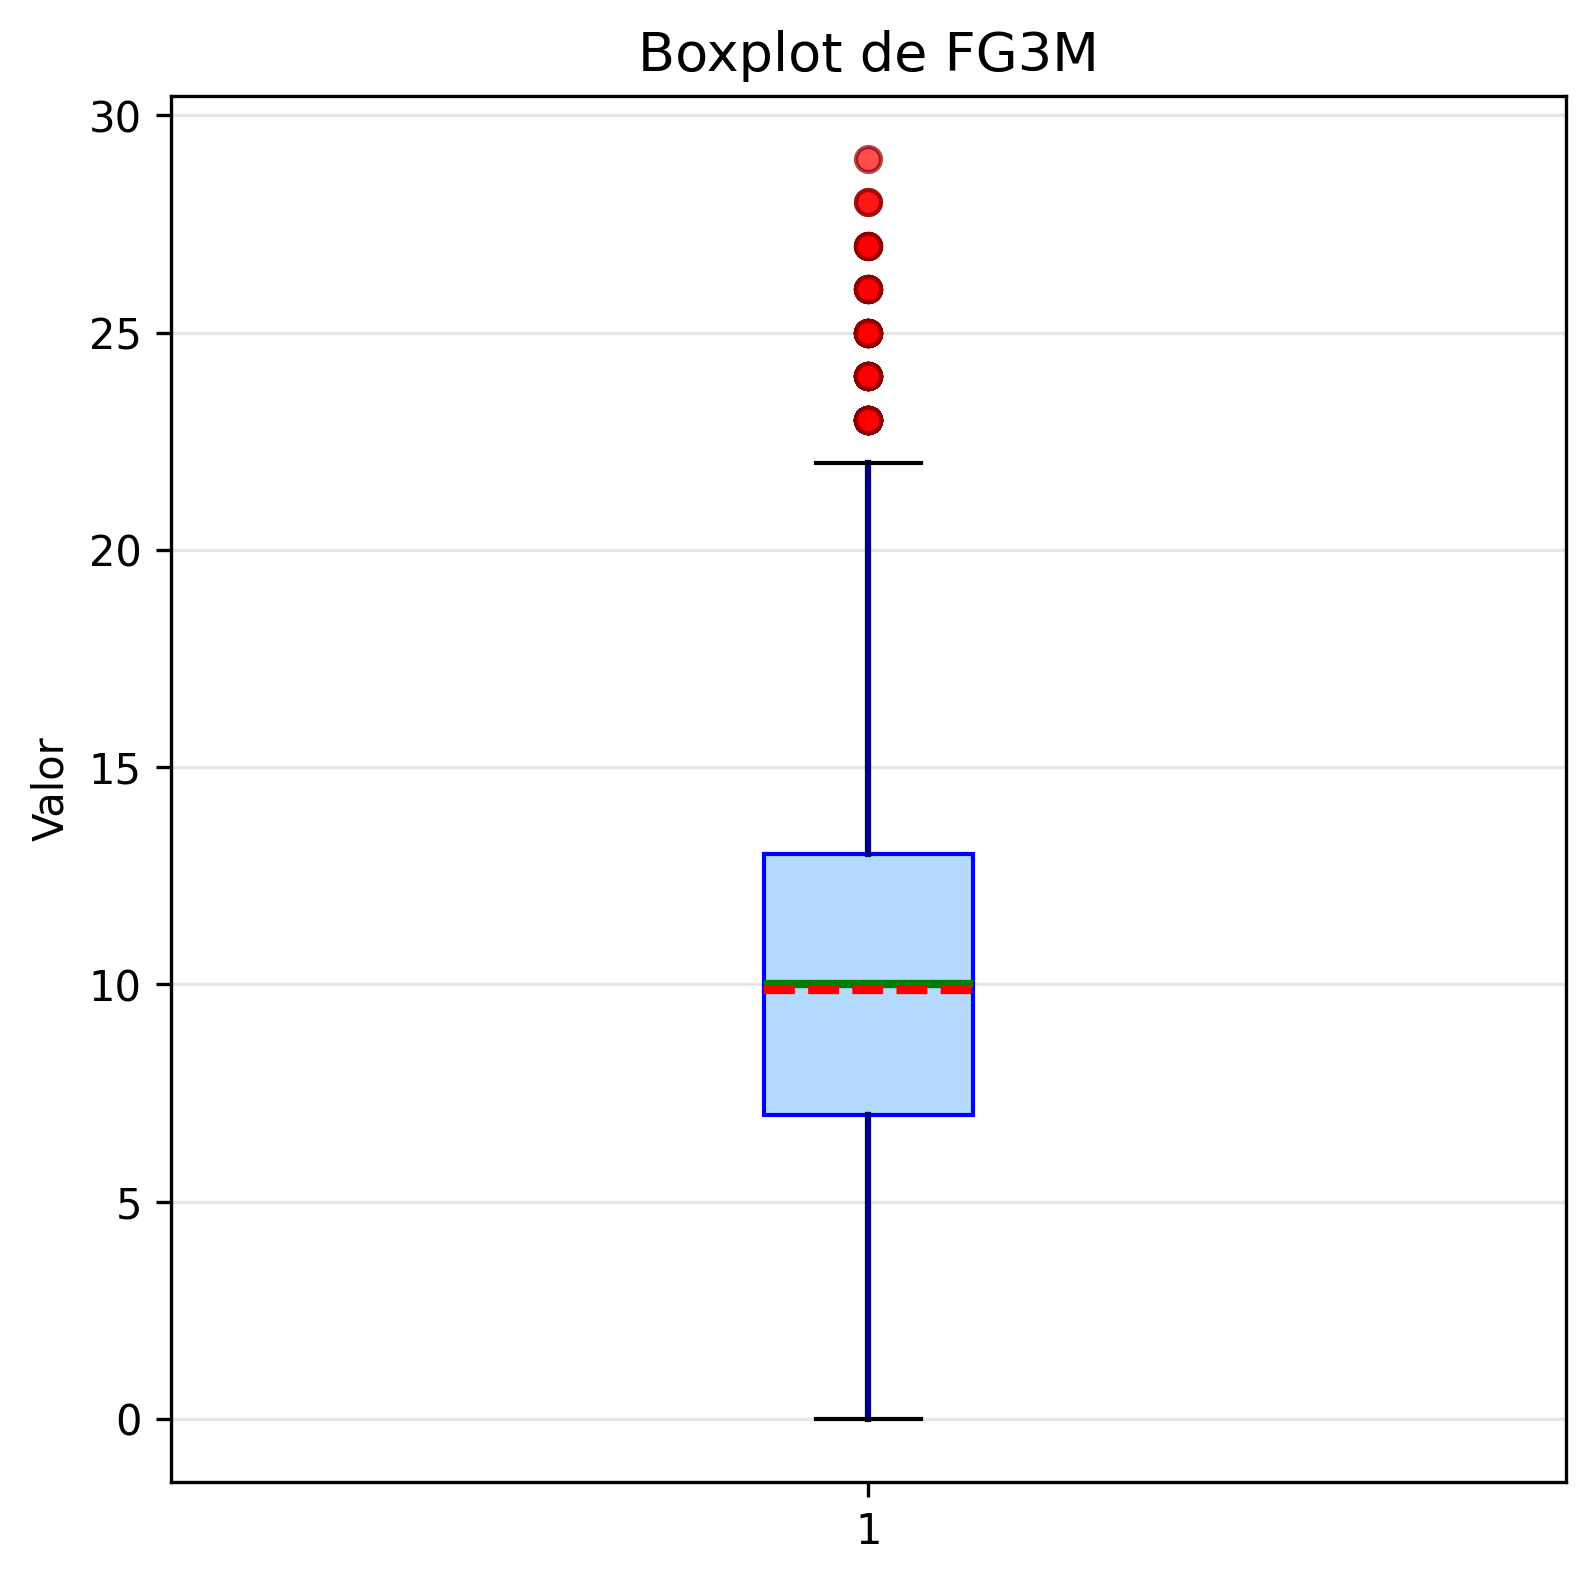
\includegraphics[width=\textwidth]{images/boxplots/boxplot_FG3M.png}
        \caption{FG3M}
        \label{fig:FG3M}
    \end{subfigure}
    \hfill
    \begin{subfigure}[b]{0.3\textwidth}
        \centering
        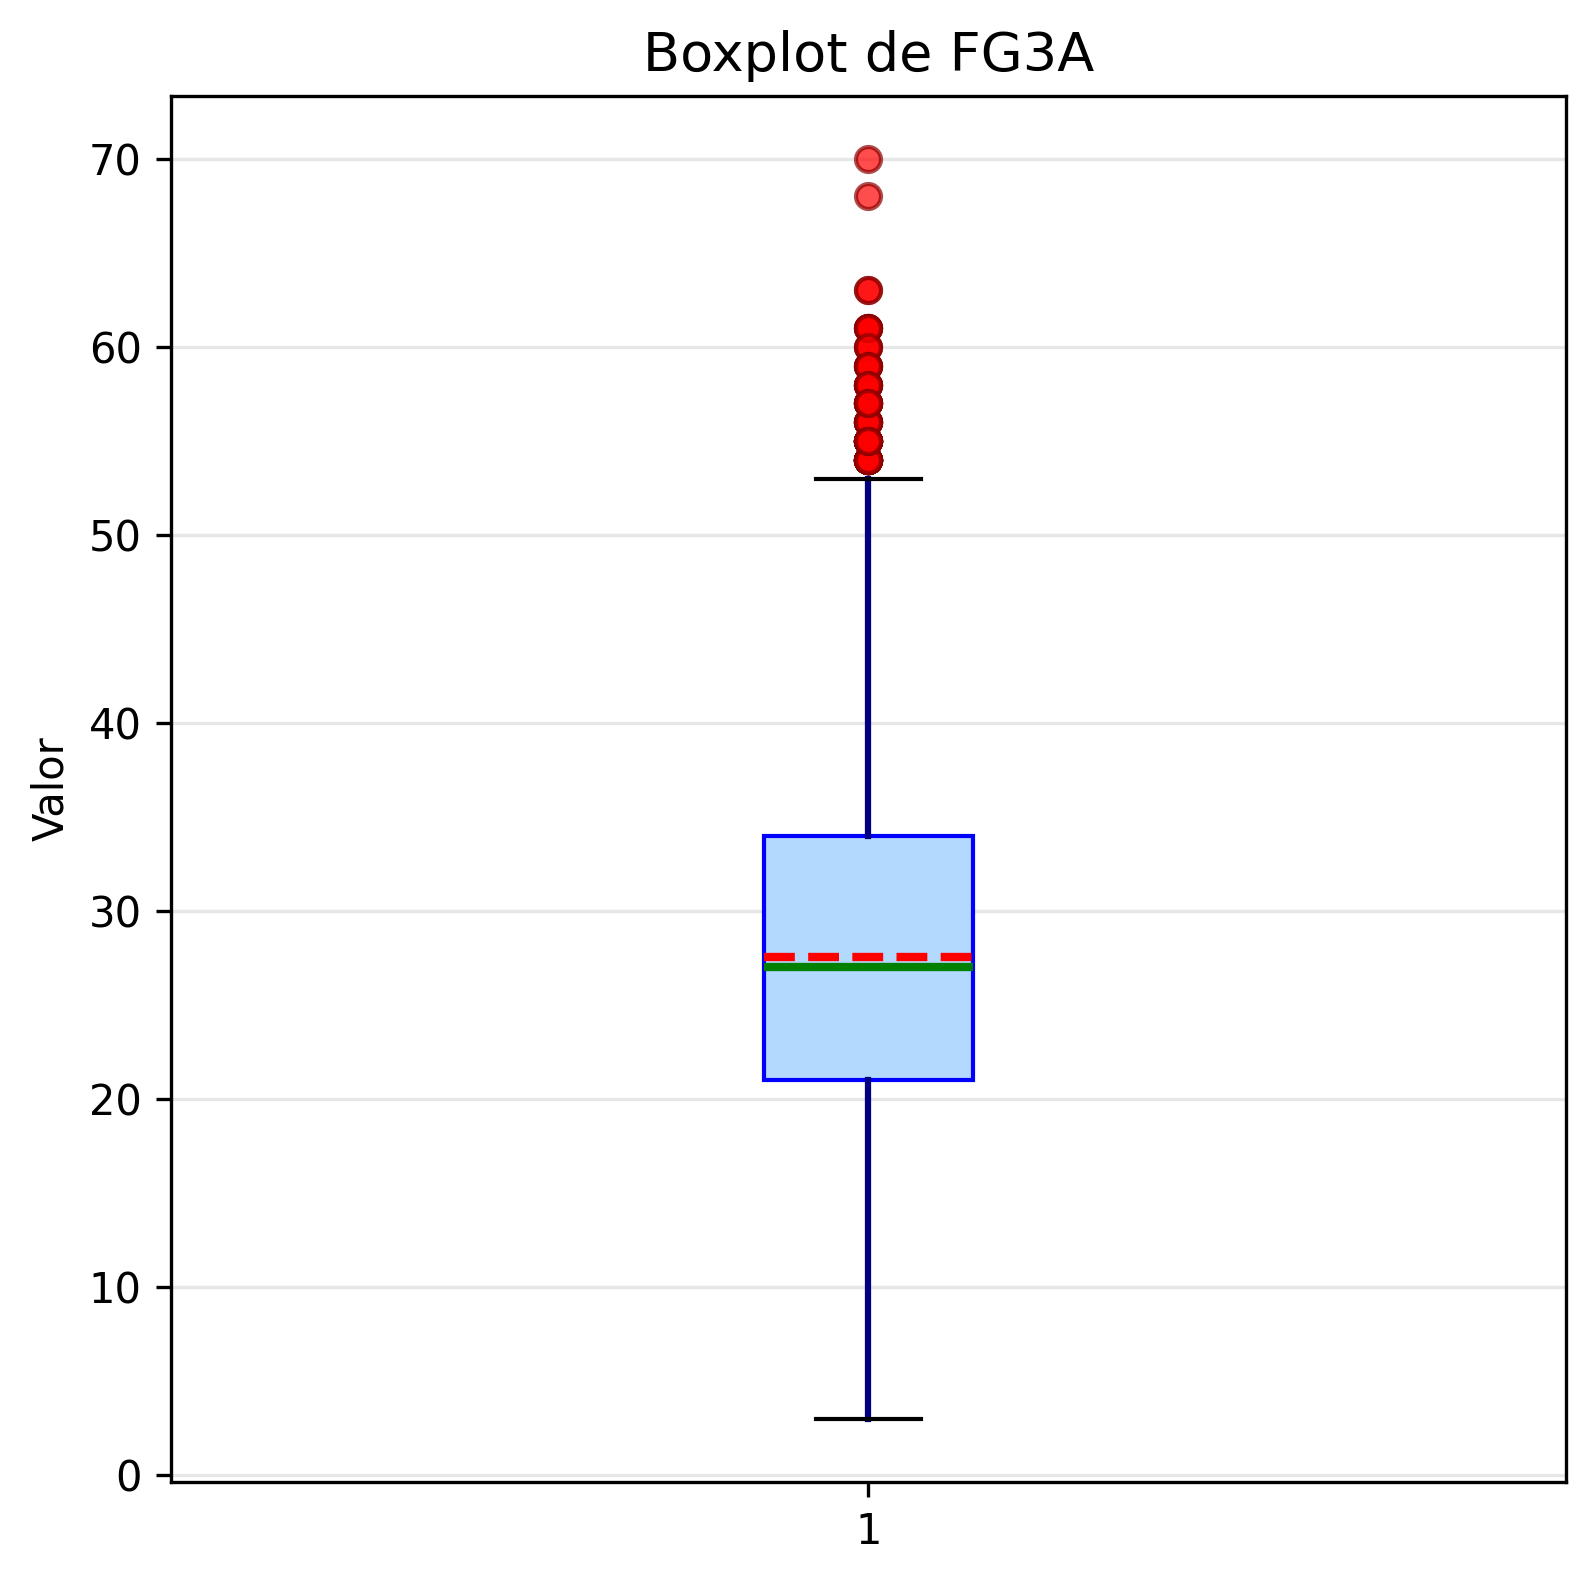
\includegraphics[width=\textwidth]{images/boxplots/boxplot_FG3A.png}
        \caption{FG3A}
        \label{fig:FG3A}
    \end{subfigure}

    \vspace{0.5cm}

    \begin{subfigure}[b]{0.3\textwidth}
        \centering
        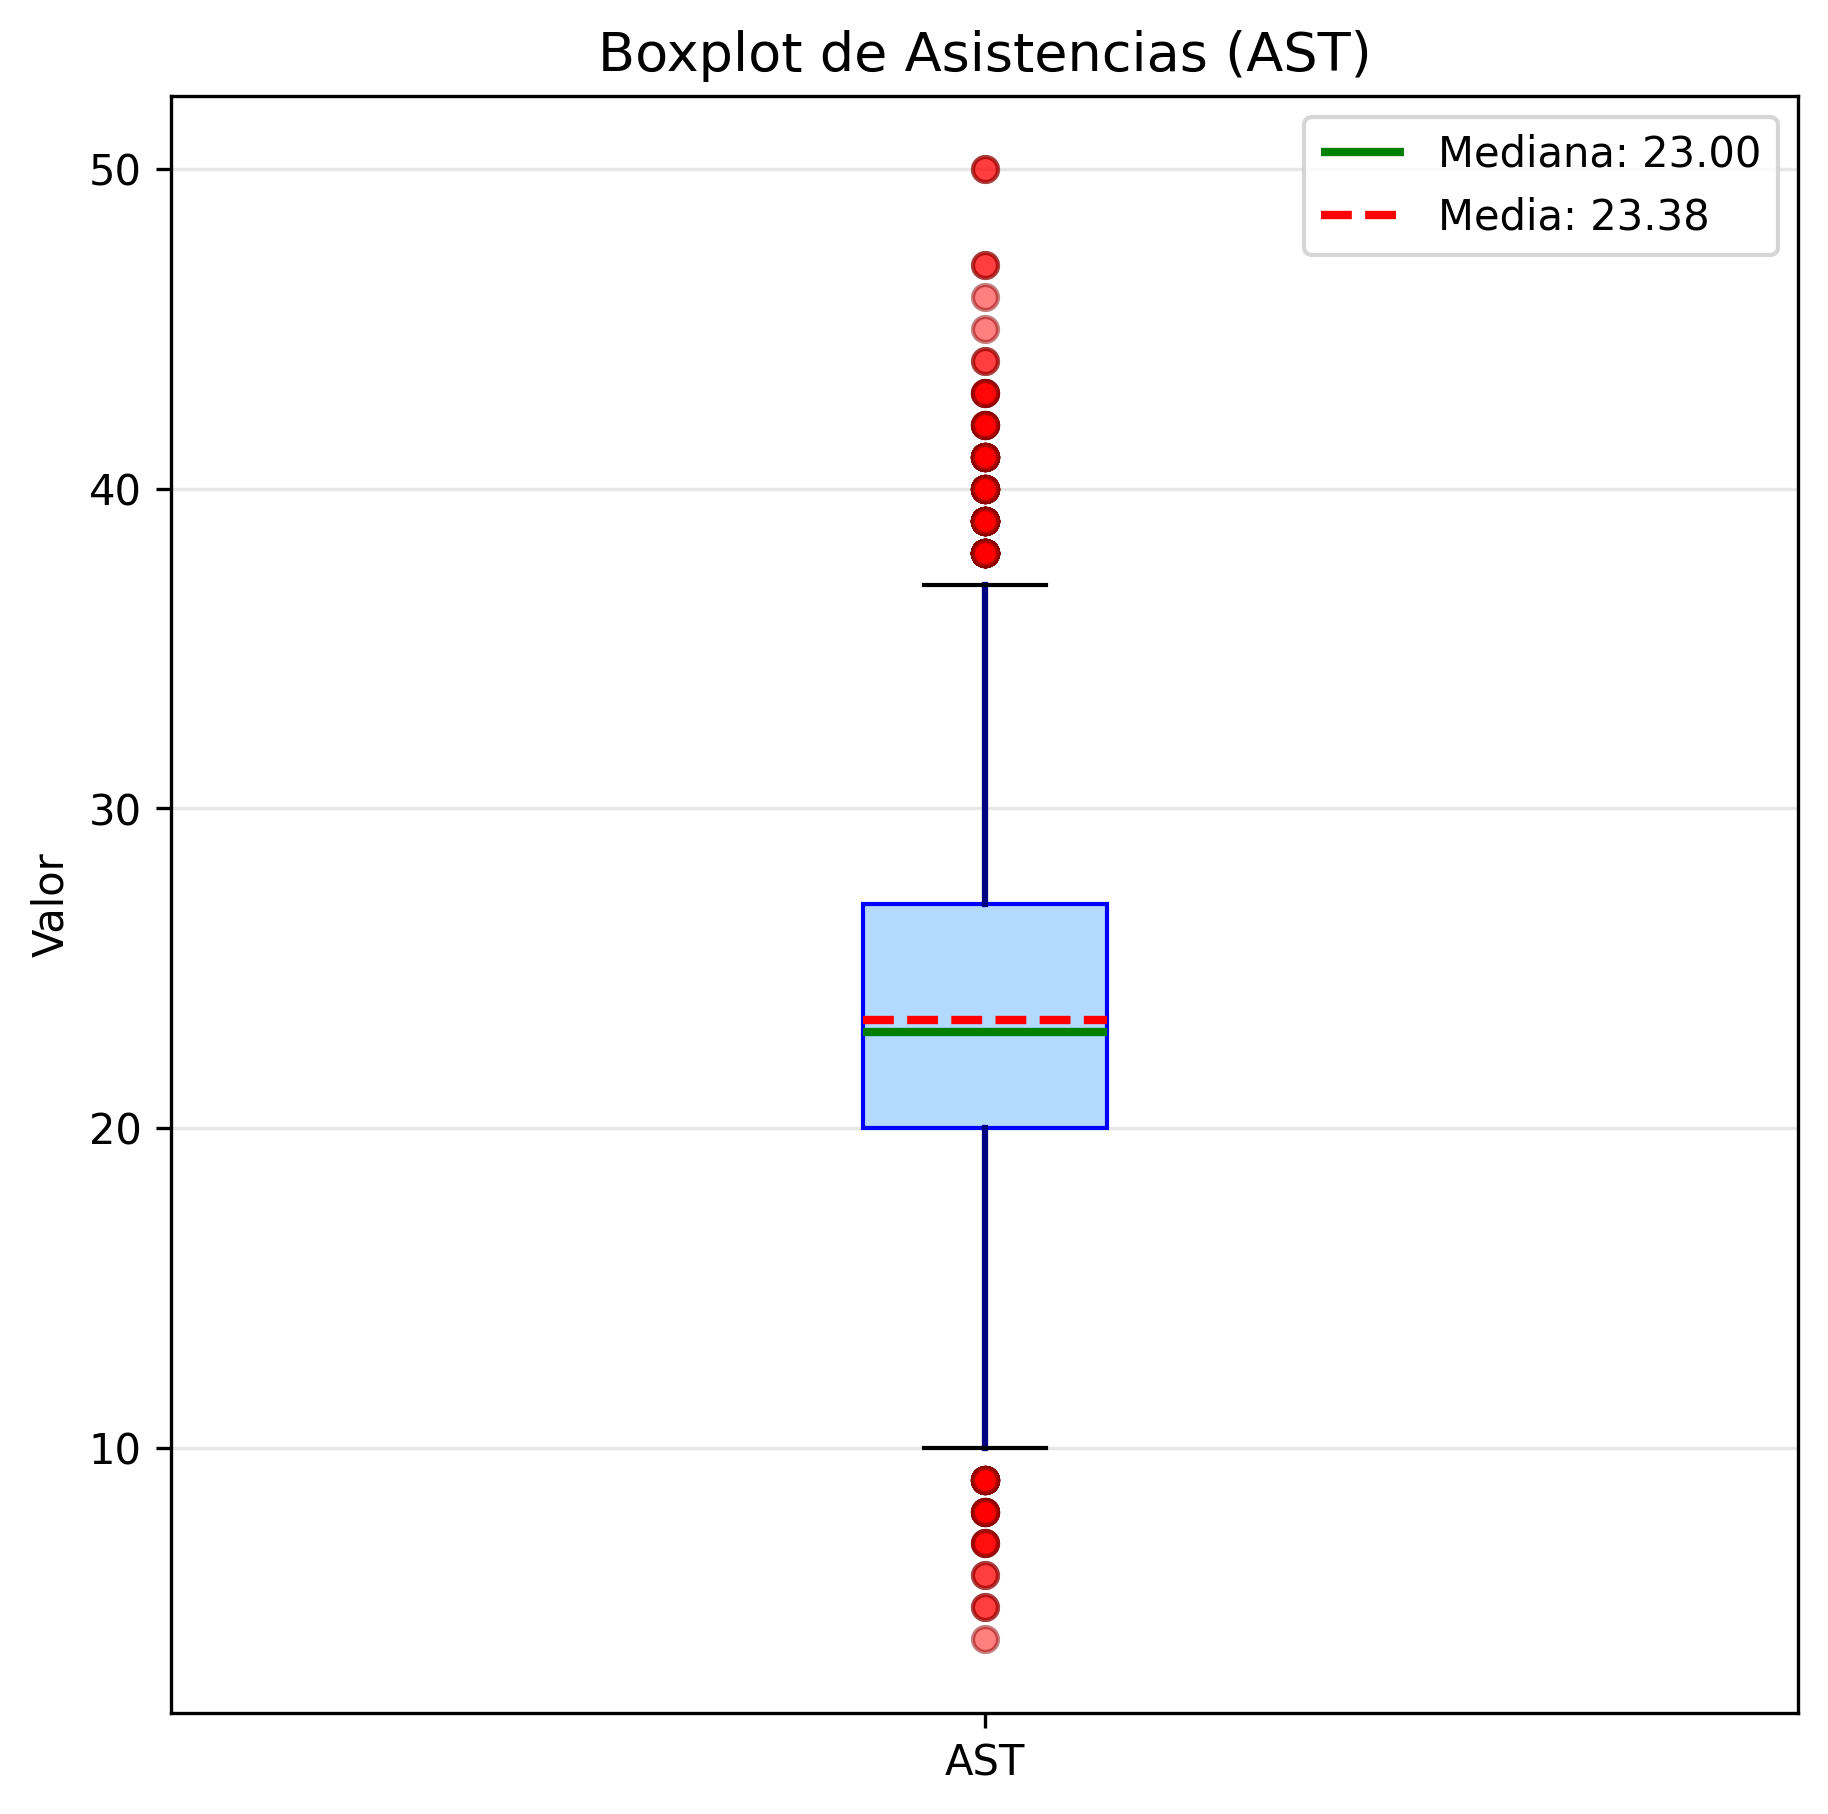
\includegraphics[width=\textwidth]{images/boxplots/boxplot_AST.png}
        \caption{AST}
        \label{fig:AST}
    \end{subfigure}
    \hfill
    \begin{subfigure}[b]{0.3\textwidth}
        \centering
        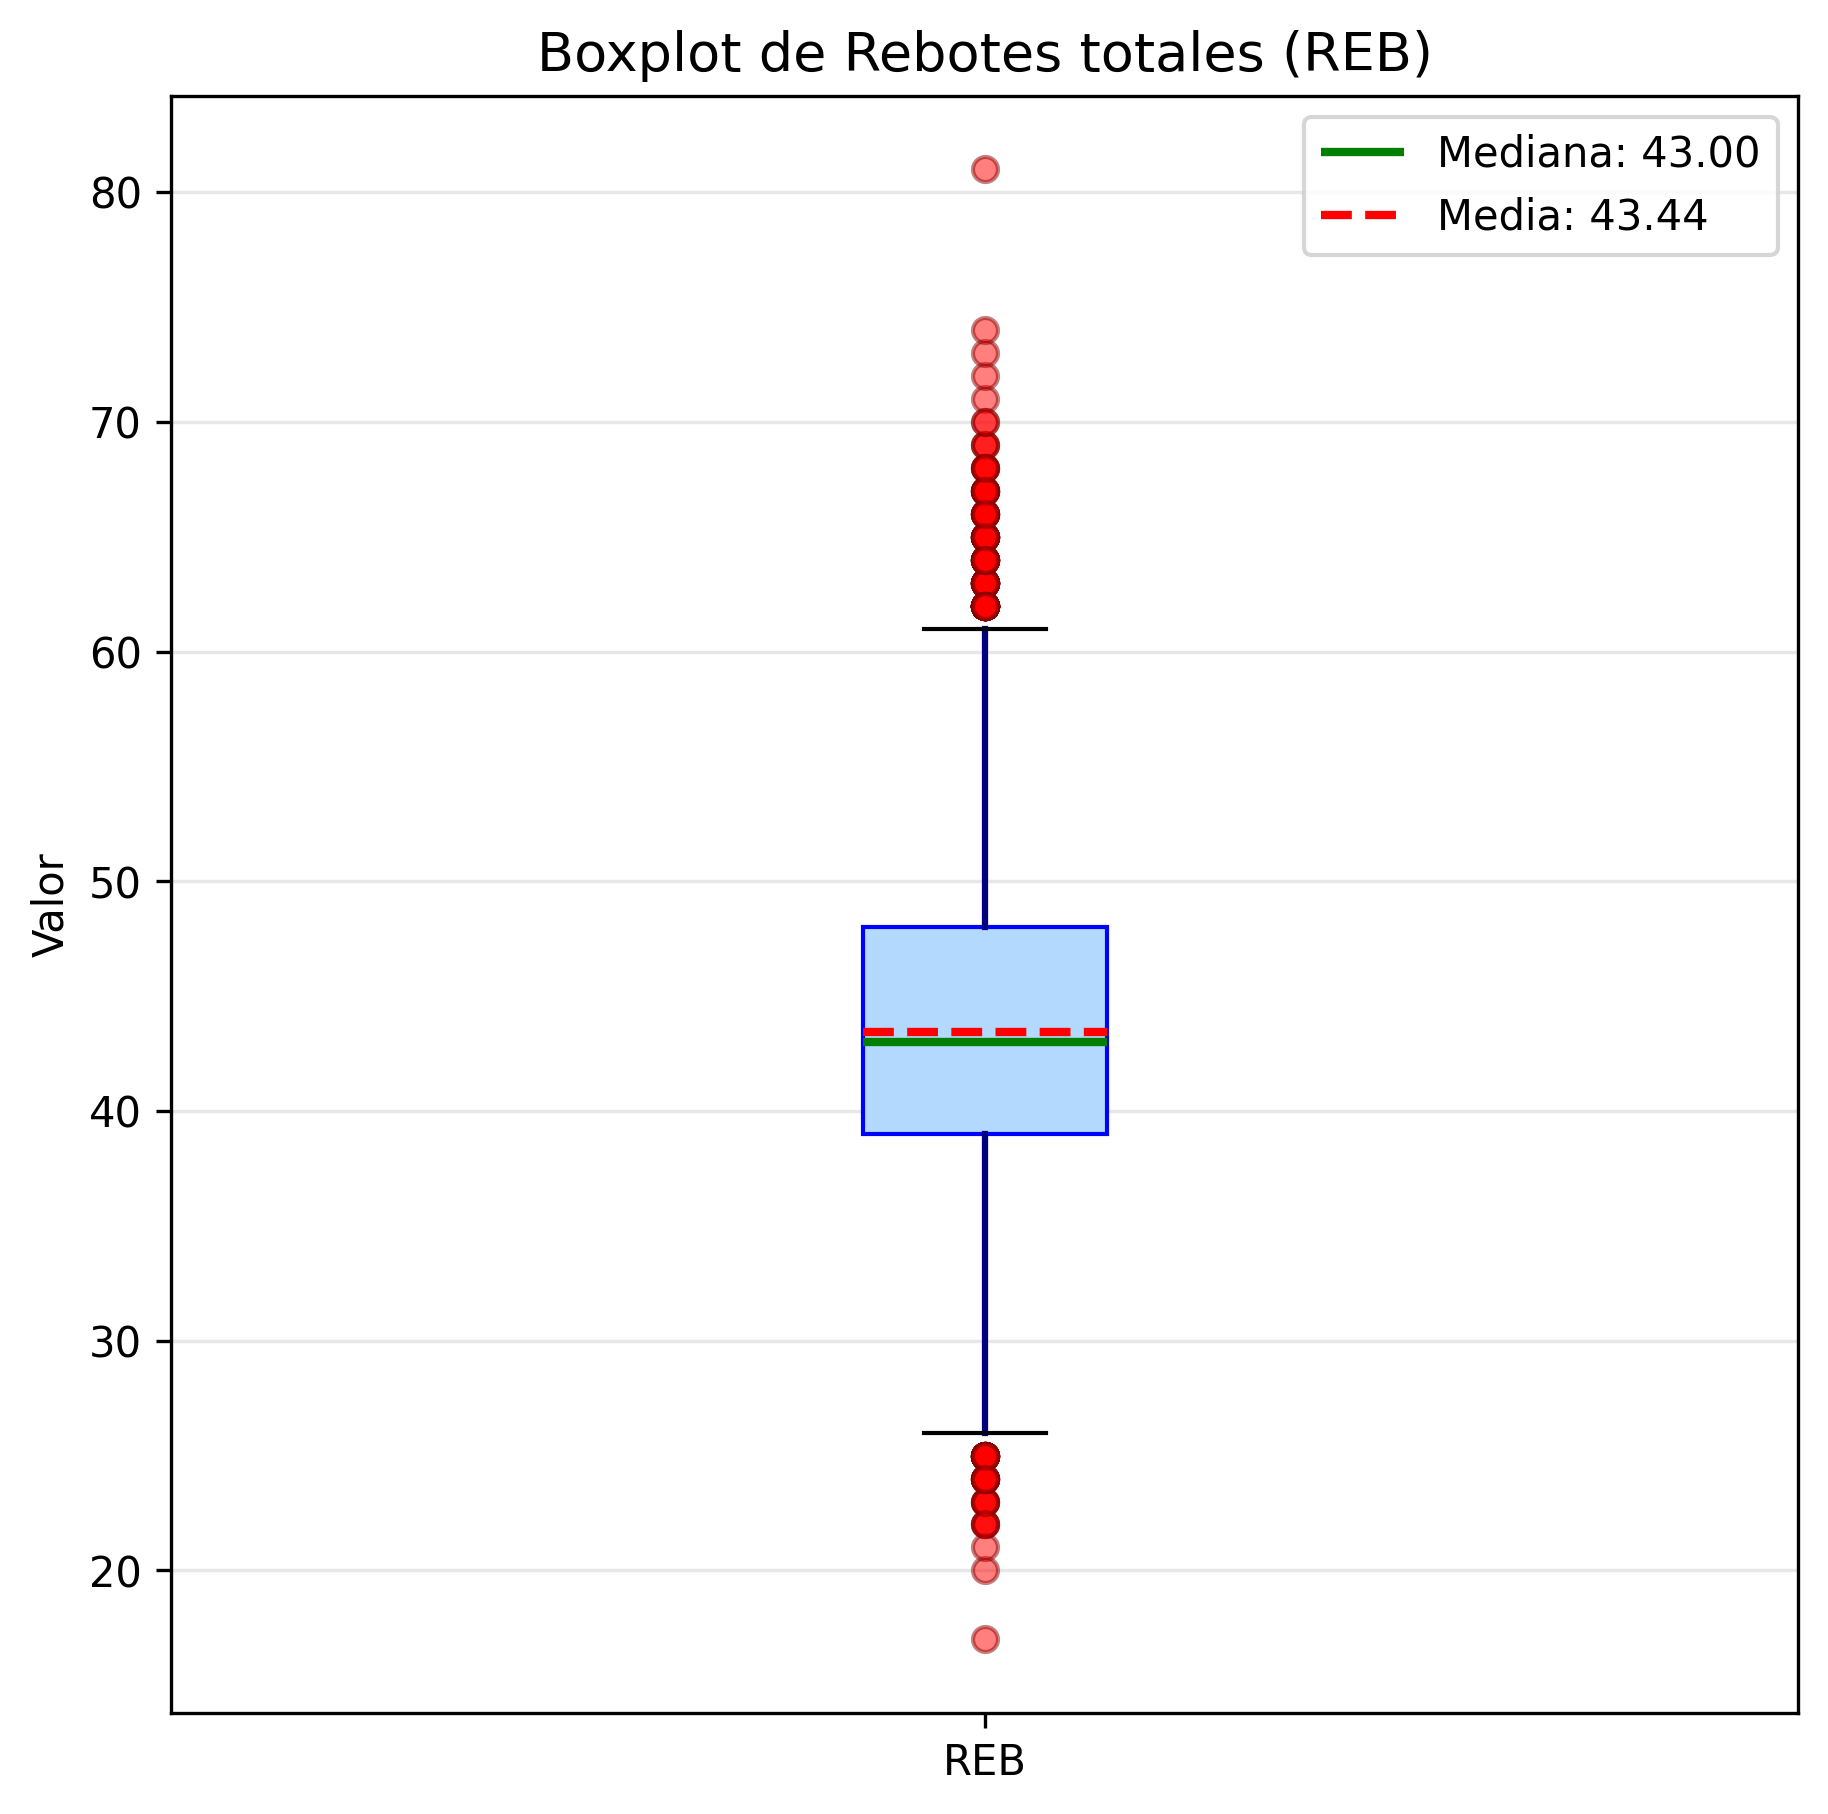
\includegraphics[width=\textwidth]{images/boxplots/boxplot_REB.png}
        \caption{REB}
        \label{fig:REB}
    \end{subfigure}
    \hfill
    \begin{subfigure}[b]{0.3\textwidth}
        \centering
        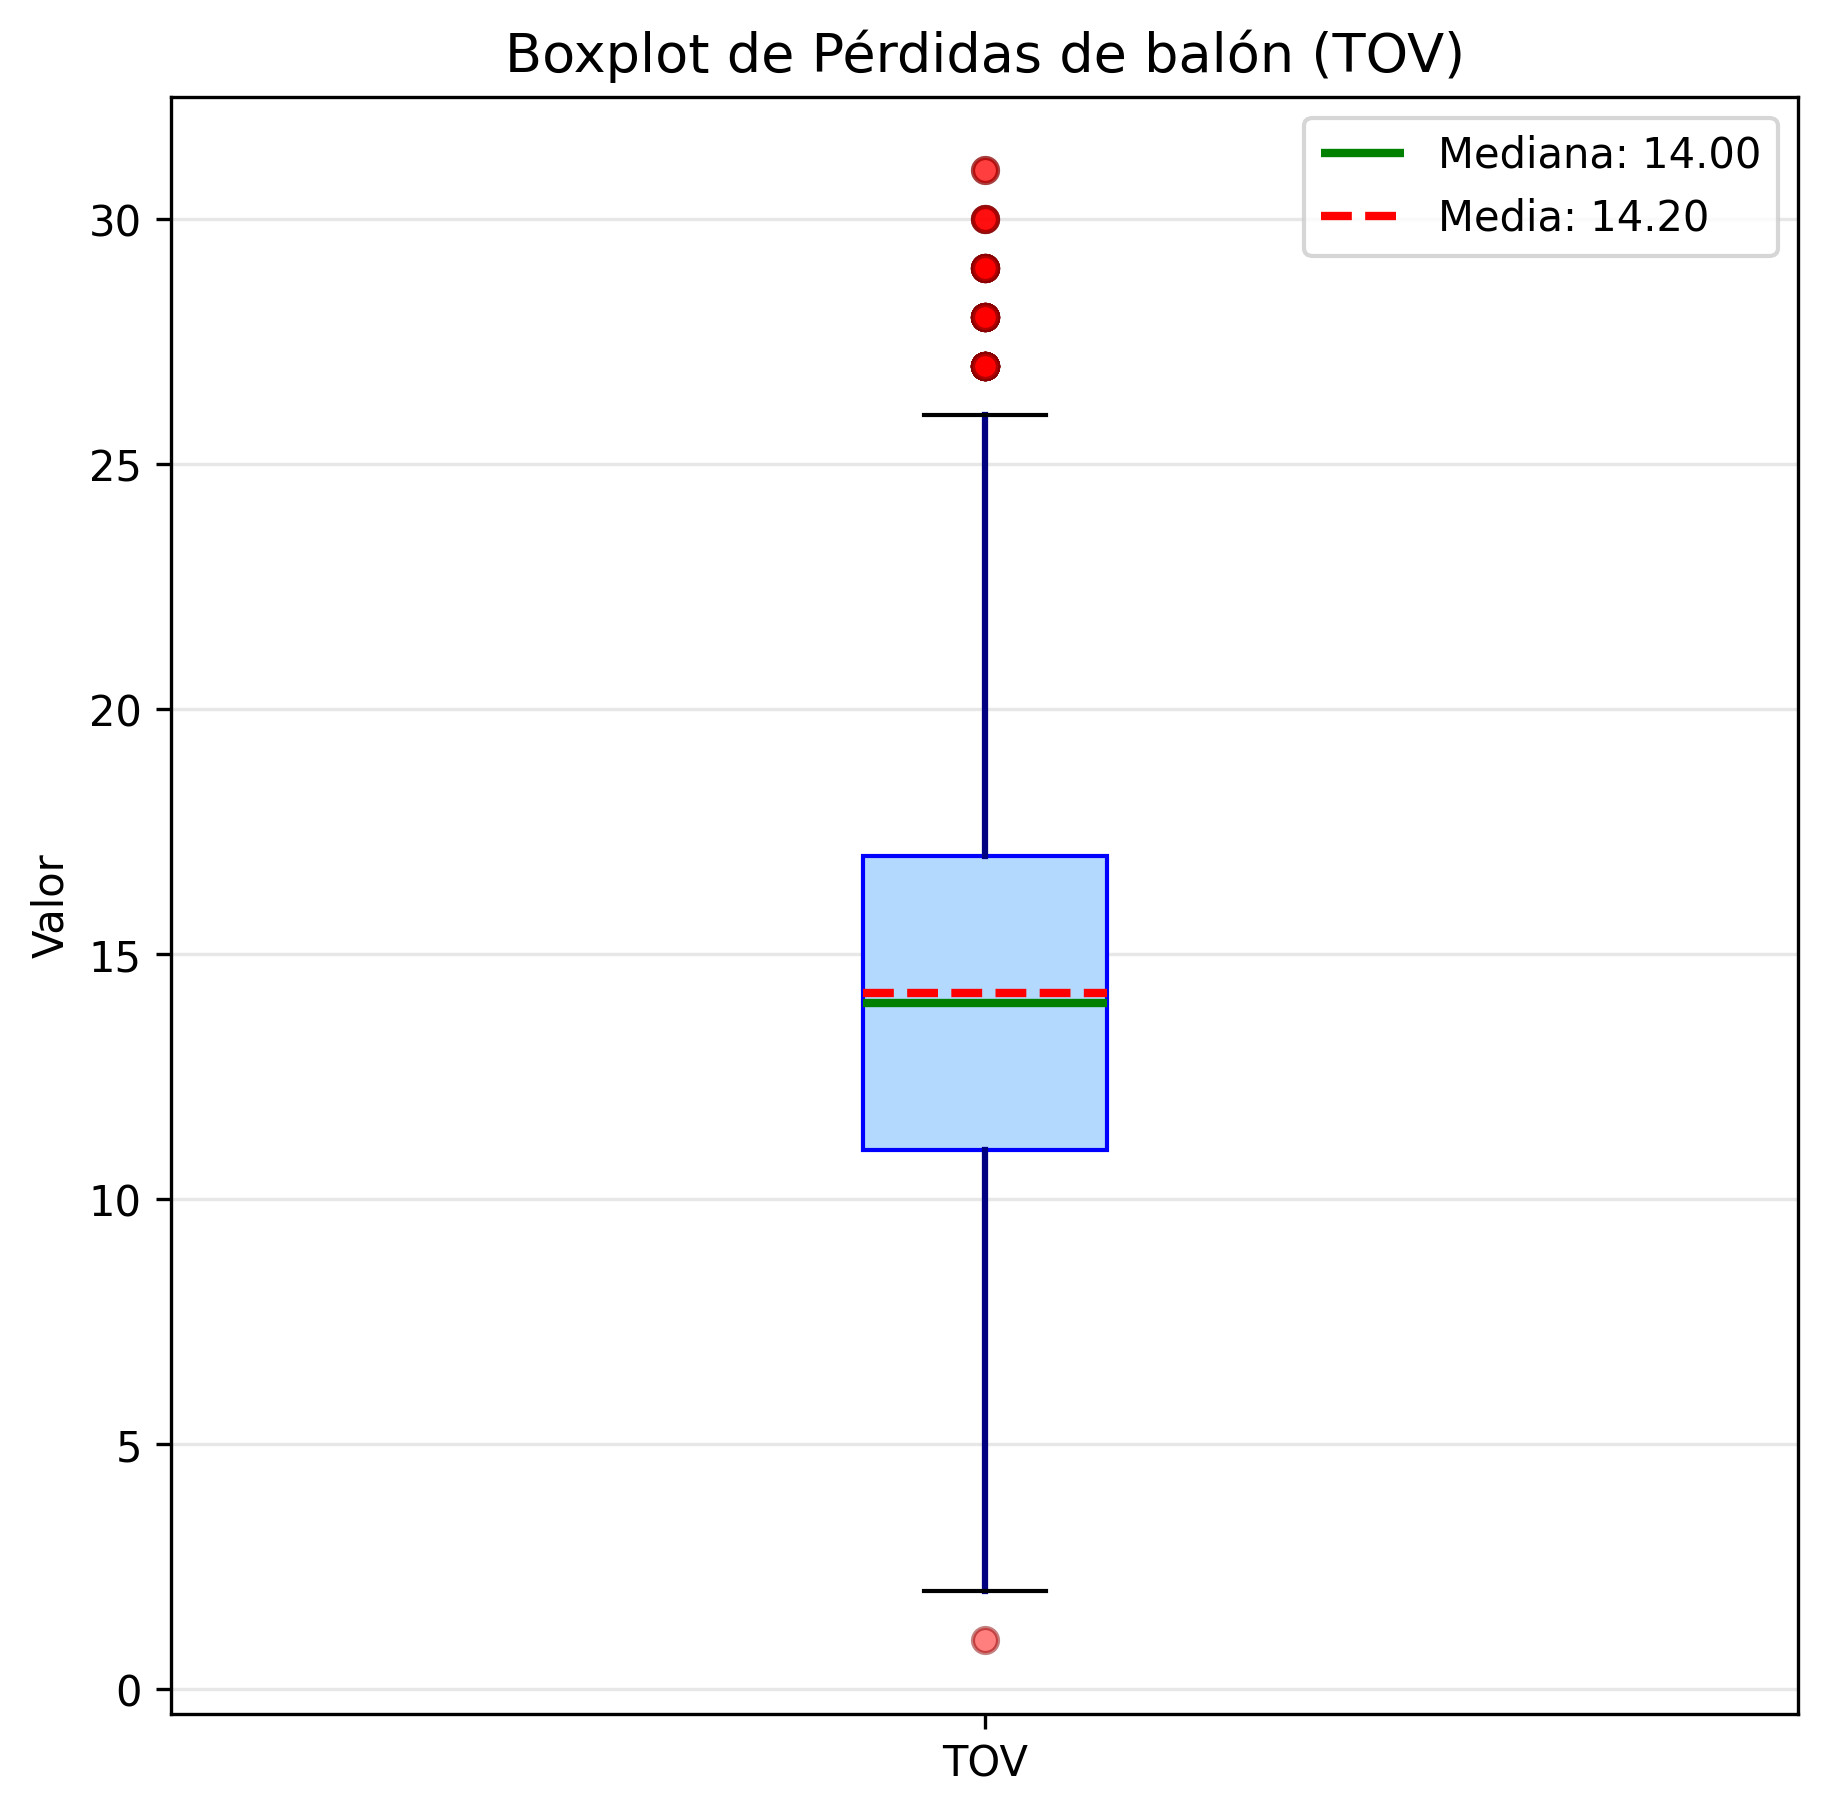
\includegraphics[width=\textwidth]{images/boxplots/boxplot_TOV.png}
        \caption{TOV}
        \label{fig:TOV}
    \end{subfigure}

    \caption{Boxplots representativos del grupo de métricas de volumen ofensivo, tiro exterior y control del juego.}
    \label{fig:boxplots_volumen_control}
\end{figure}

\subsubsection*{Resumen del grupo: métricas de eficiencia y perfil de tiro}

Las variables incluidas en este grupo (\textit{FG\_PCT, FG3\_PCT, FT\_PCT y FG3A/FGA}) describen la
\textbf{eficiencia ofensiva y la orientación del lanzamiento} del equipo. En conjunto, los
boxplots muestran distribuciones claramente más concentradas que las observadas en métricas de
volumen, lo que refleja una mayor estabilidad relativa en los porcentajes de acierto a lo largo
de los partidos analizados.

Un rasgo común del grupo es la \textbf{proximidad entre media y mediana}, lo que sugiere
distribuciones aproximadamente simétricas y un comportamiento consistente en términos de
eficiencia. Sin embargo, se observa una diferencia clara entre métricas: \textit{FG\_PCT} y
\textit{FT\_PCT} presentan rangos intercuartílicos reducidos, indicando una elevada estabilidad,
mientras que \textit{FG3\_PCT} exhibe una dispersión notablemente mayor, confirmando el carácter
más volátil del tiro de tres puntos.

La variable \textit{FG3A/FGA} aporta una perspectiva complementaria al describir el
\textbf{perfil táctico de lanzamiento} más que la eficiencia en sí. Su dispersión moderada y la
escasa presencia de valores atípicos sugieren que, aunque existen variaciones estratégicas entre
partidos, la proporción de tiros de tres puntos se mantiene dentro de un rango relativamente
homogéneo.

En conjunto, estos boxplots permiten diferenciar claramente entre métricas de eficiencia estable
(\textit{FG\_PCT, FT\_PCT}), métricas altamente dependientes del contexto (\textit{FG3\_PCT}) y
métricas de estilo ofensivo (\textit{FG3A/FGA}), justificando su análisis conjunto y evitando
redundancias descriptivas mediante la presentación de una selección representativa.

\begin{figure}[H]
    \centering
    \begin{subfigure}[b]{0.45\textwidth}
        \centering
        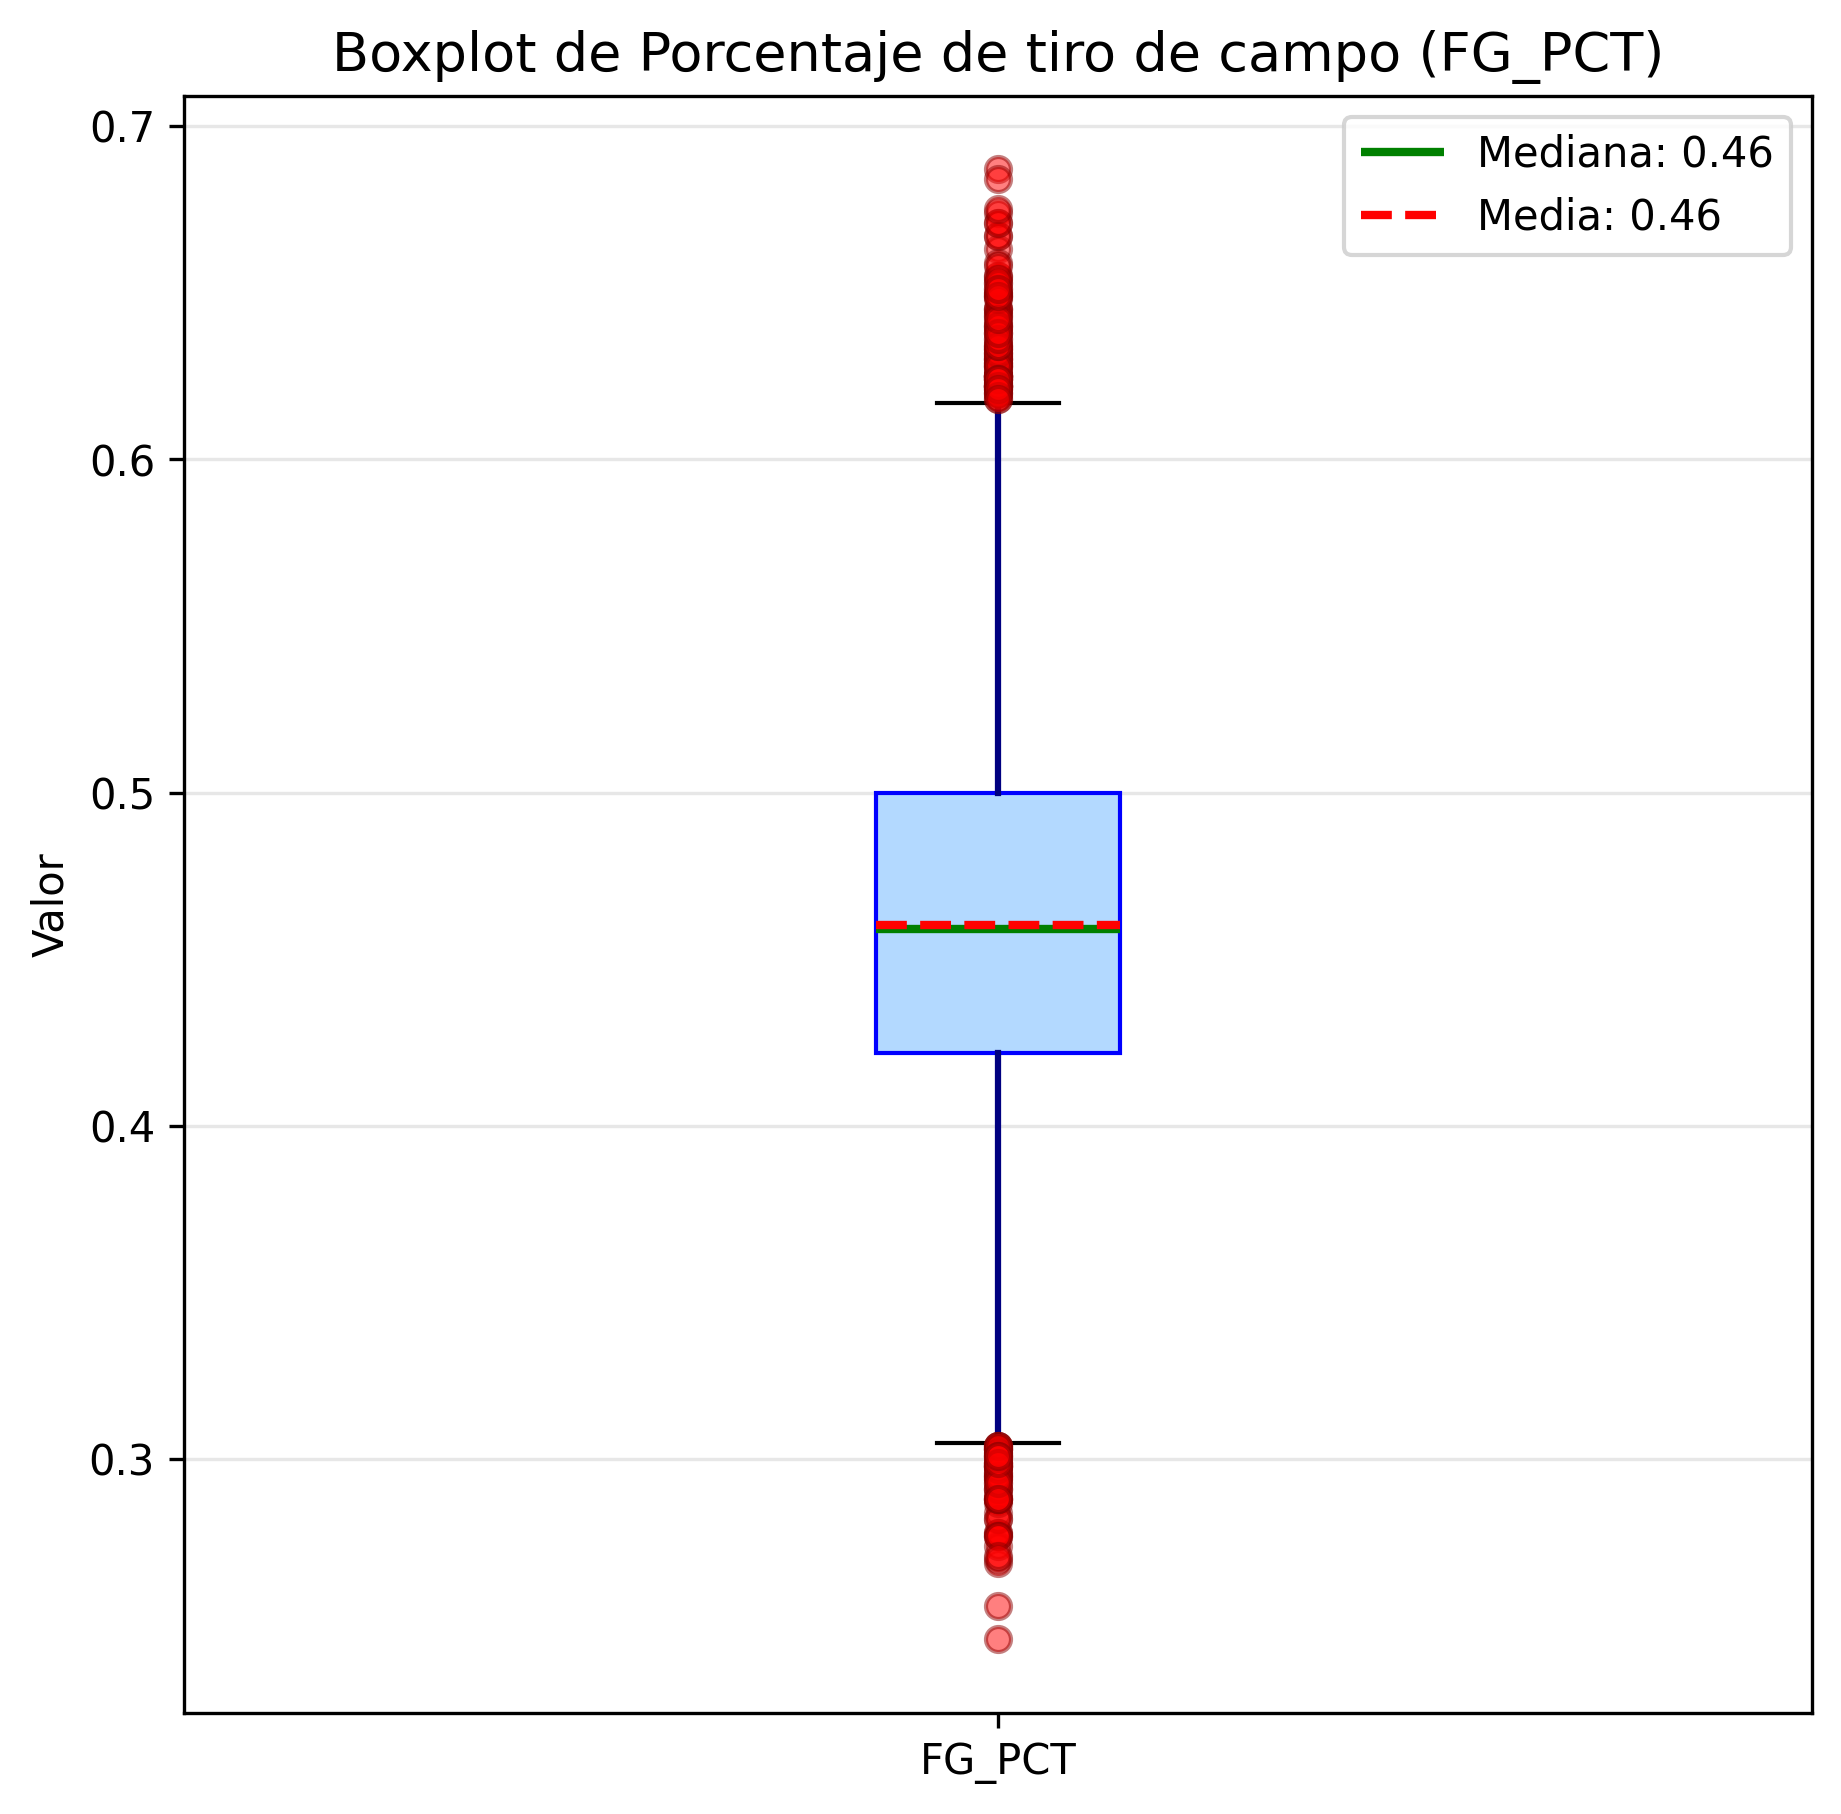
\includegraphics[width=\textwidth]{images/boxplots/boxplot_FG_PCT.png}
        \caption{FG\_PCT}
        \label{fig:FG_PCT_eff}
    \end{subfigure}
    \hfill
    \begin{subfigure}[b]{0.45\textwidth}
        \centering
        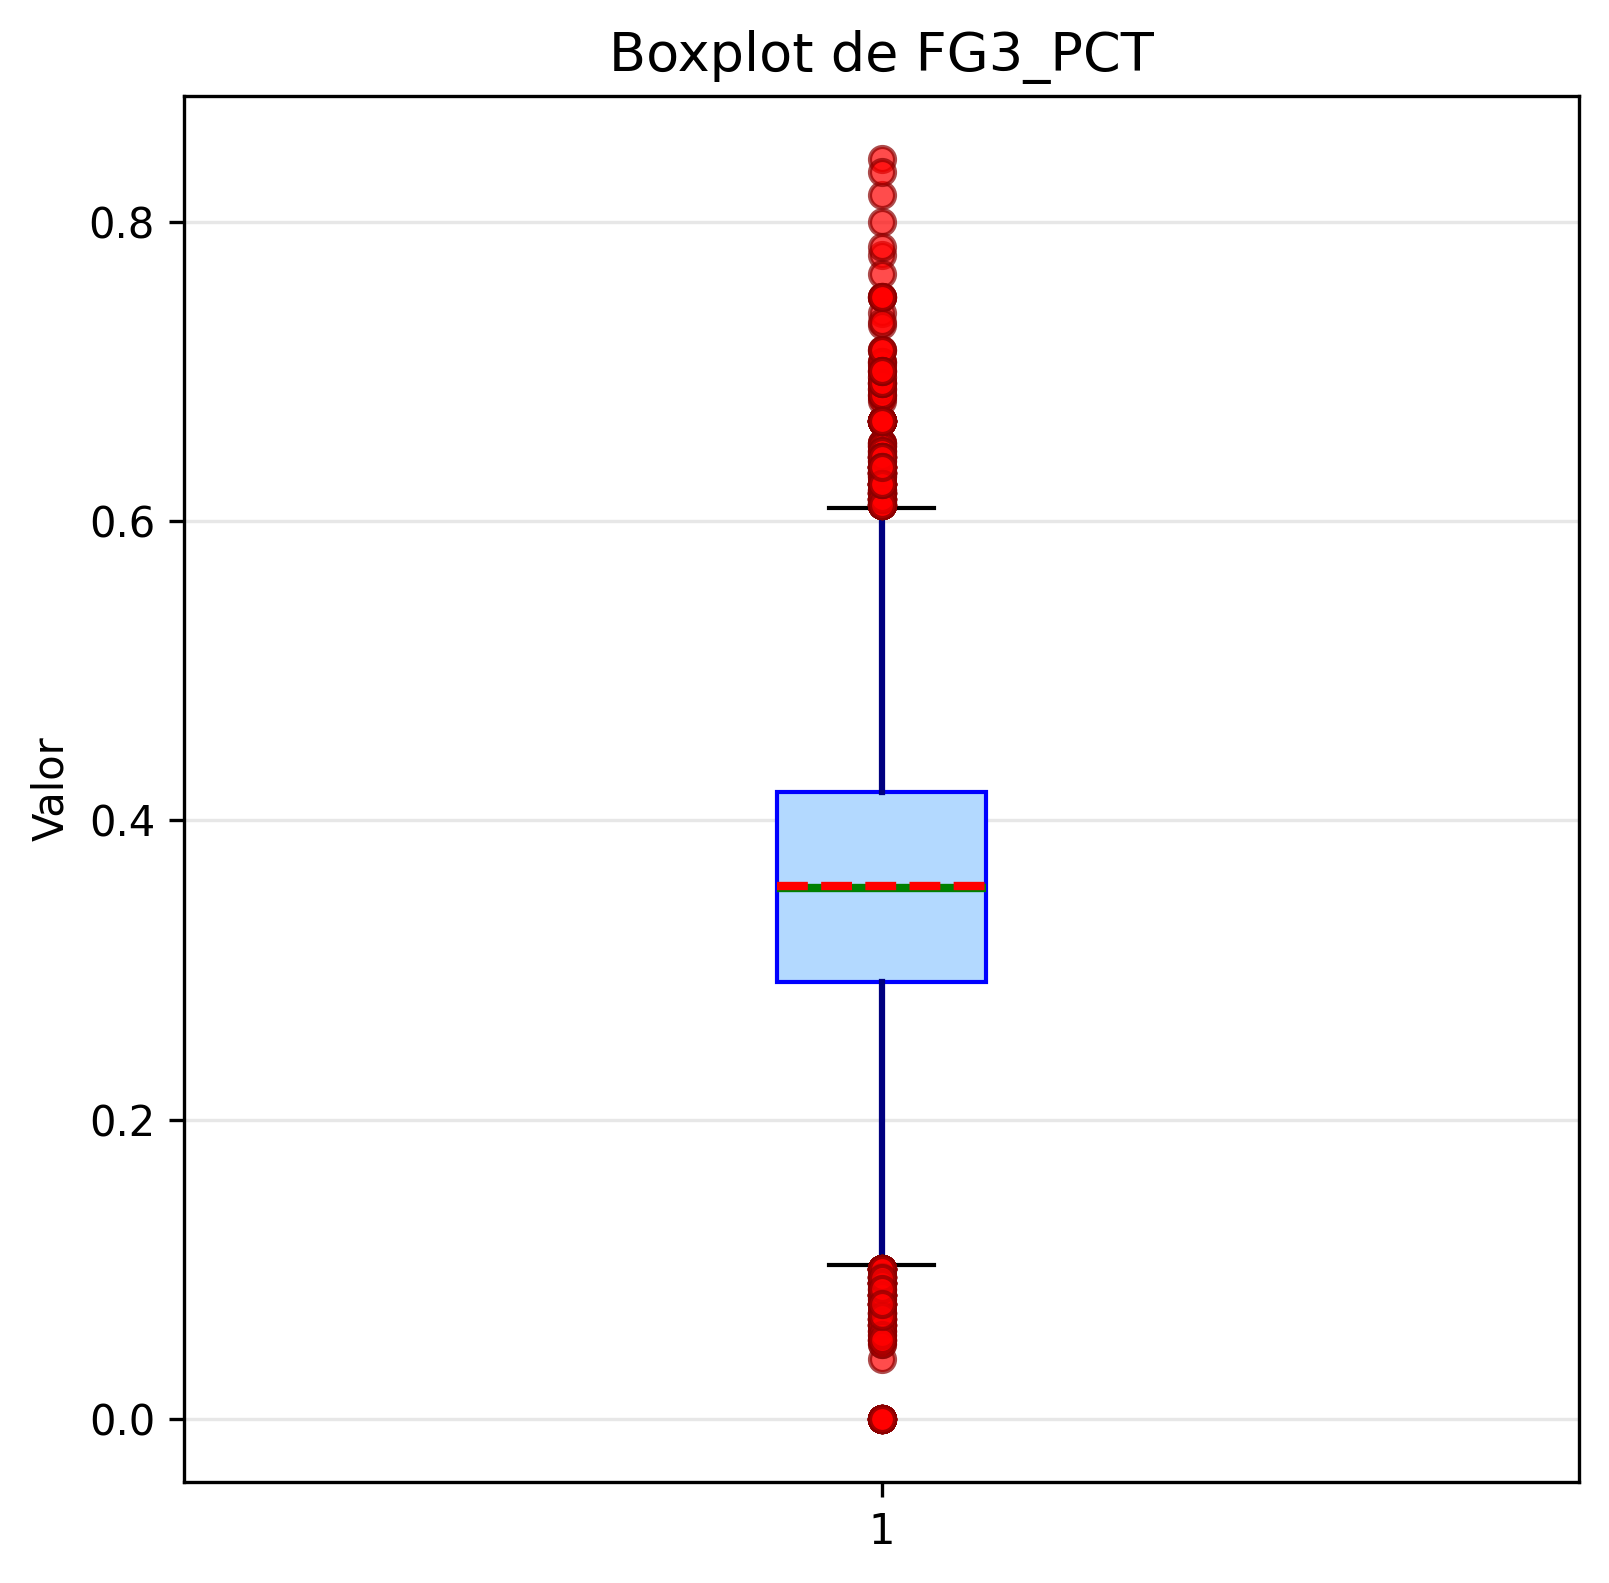
\includegraphics[width=\textwidth]{images/boxplots/boxplot_FG3_PCT.png}
        \caption{FG3\_PCT}
        \label{fig:FG3_PCT_eff}
    \end{subfigure}
    
    \vspace{0.5cm}
    
    \begin{subfigure}[b]{0.45\textwidth}
        \centering
        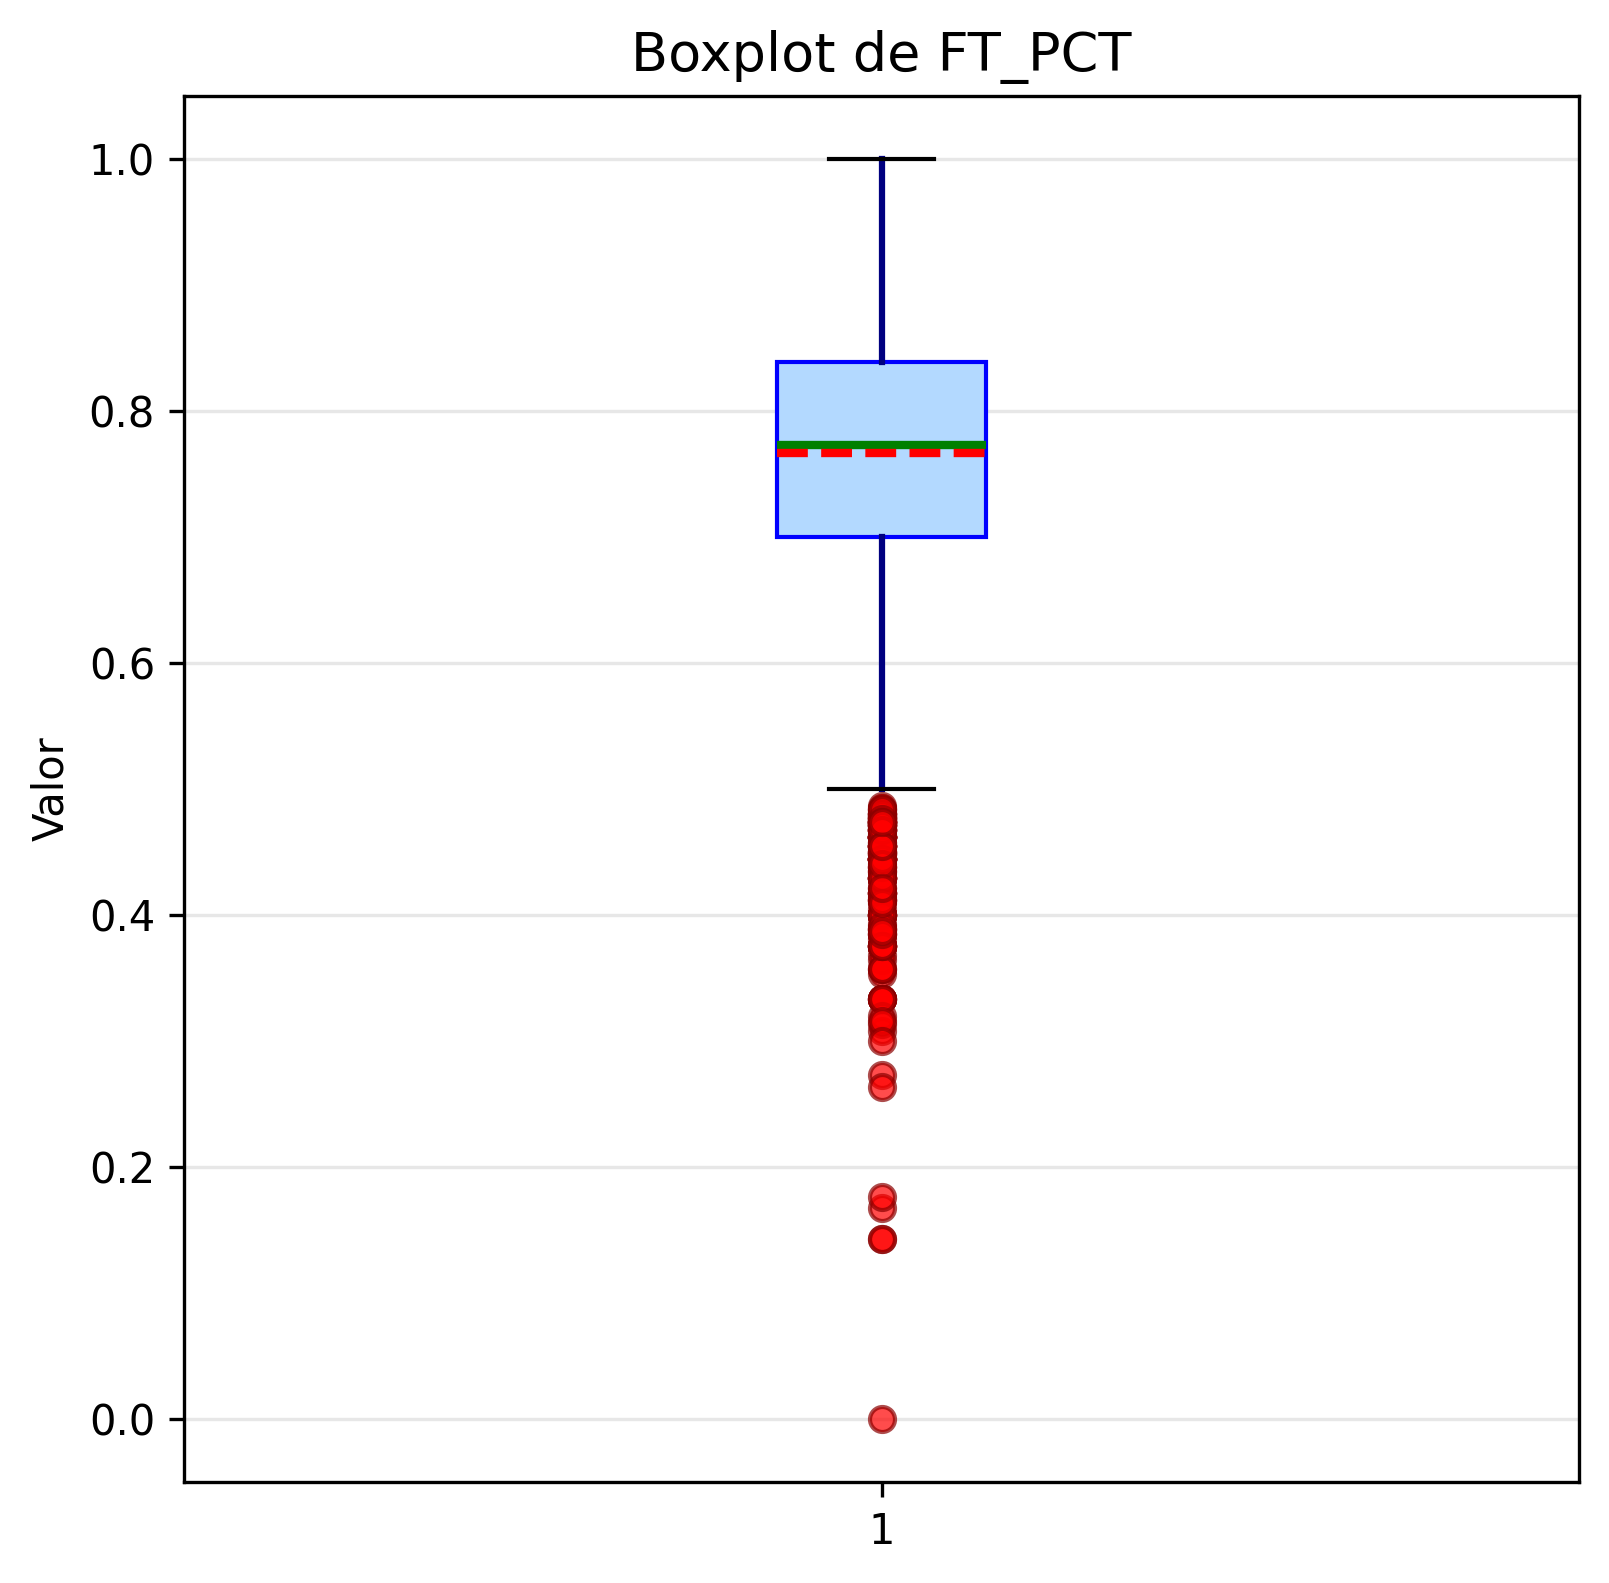
\includegraphics[width=\textwidth]{images/boxplots/boxplot_FT_PCT.png}
        \caption{FT\_PCT}
        \label{fig:FT_PCT_eff}
    \end{subfigure}
    \hfill
    \begin{subfigure}[b]{0.45\textwidth}
        \centering
        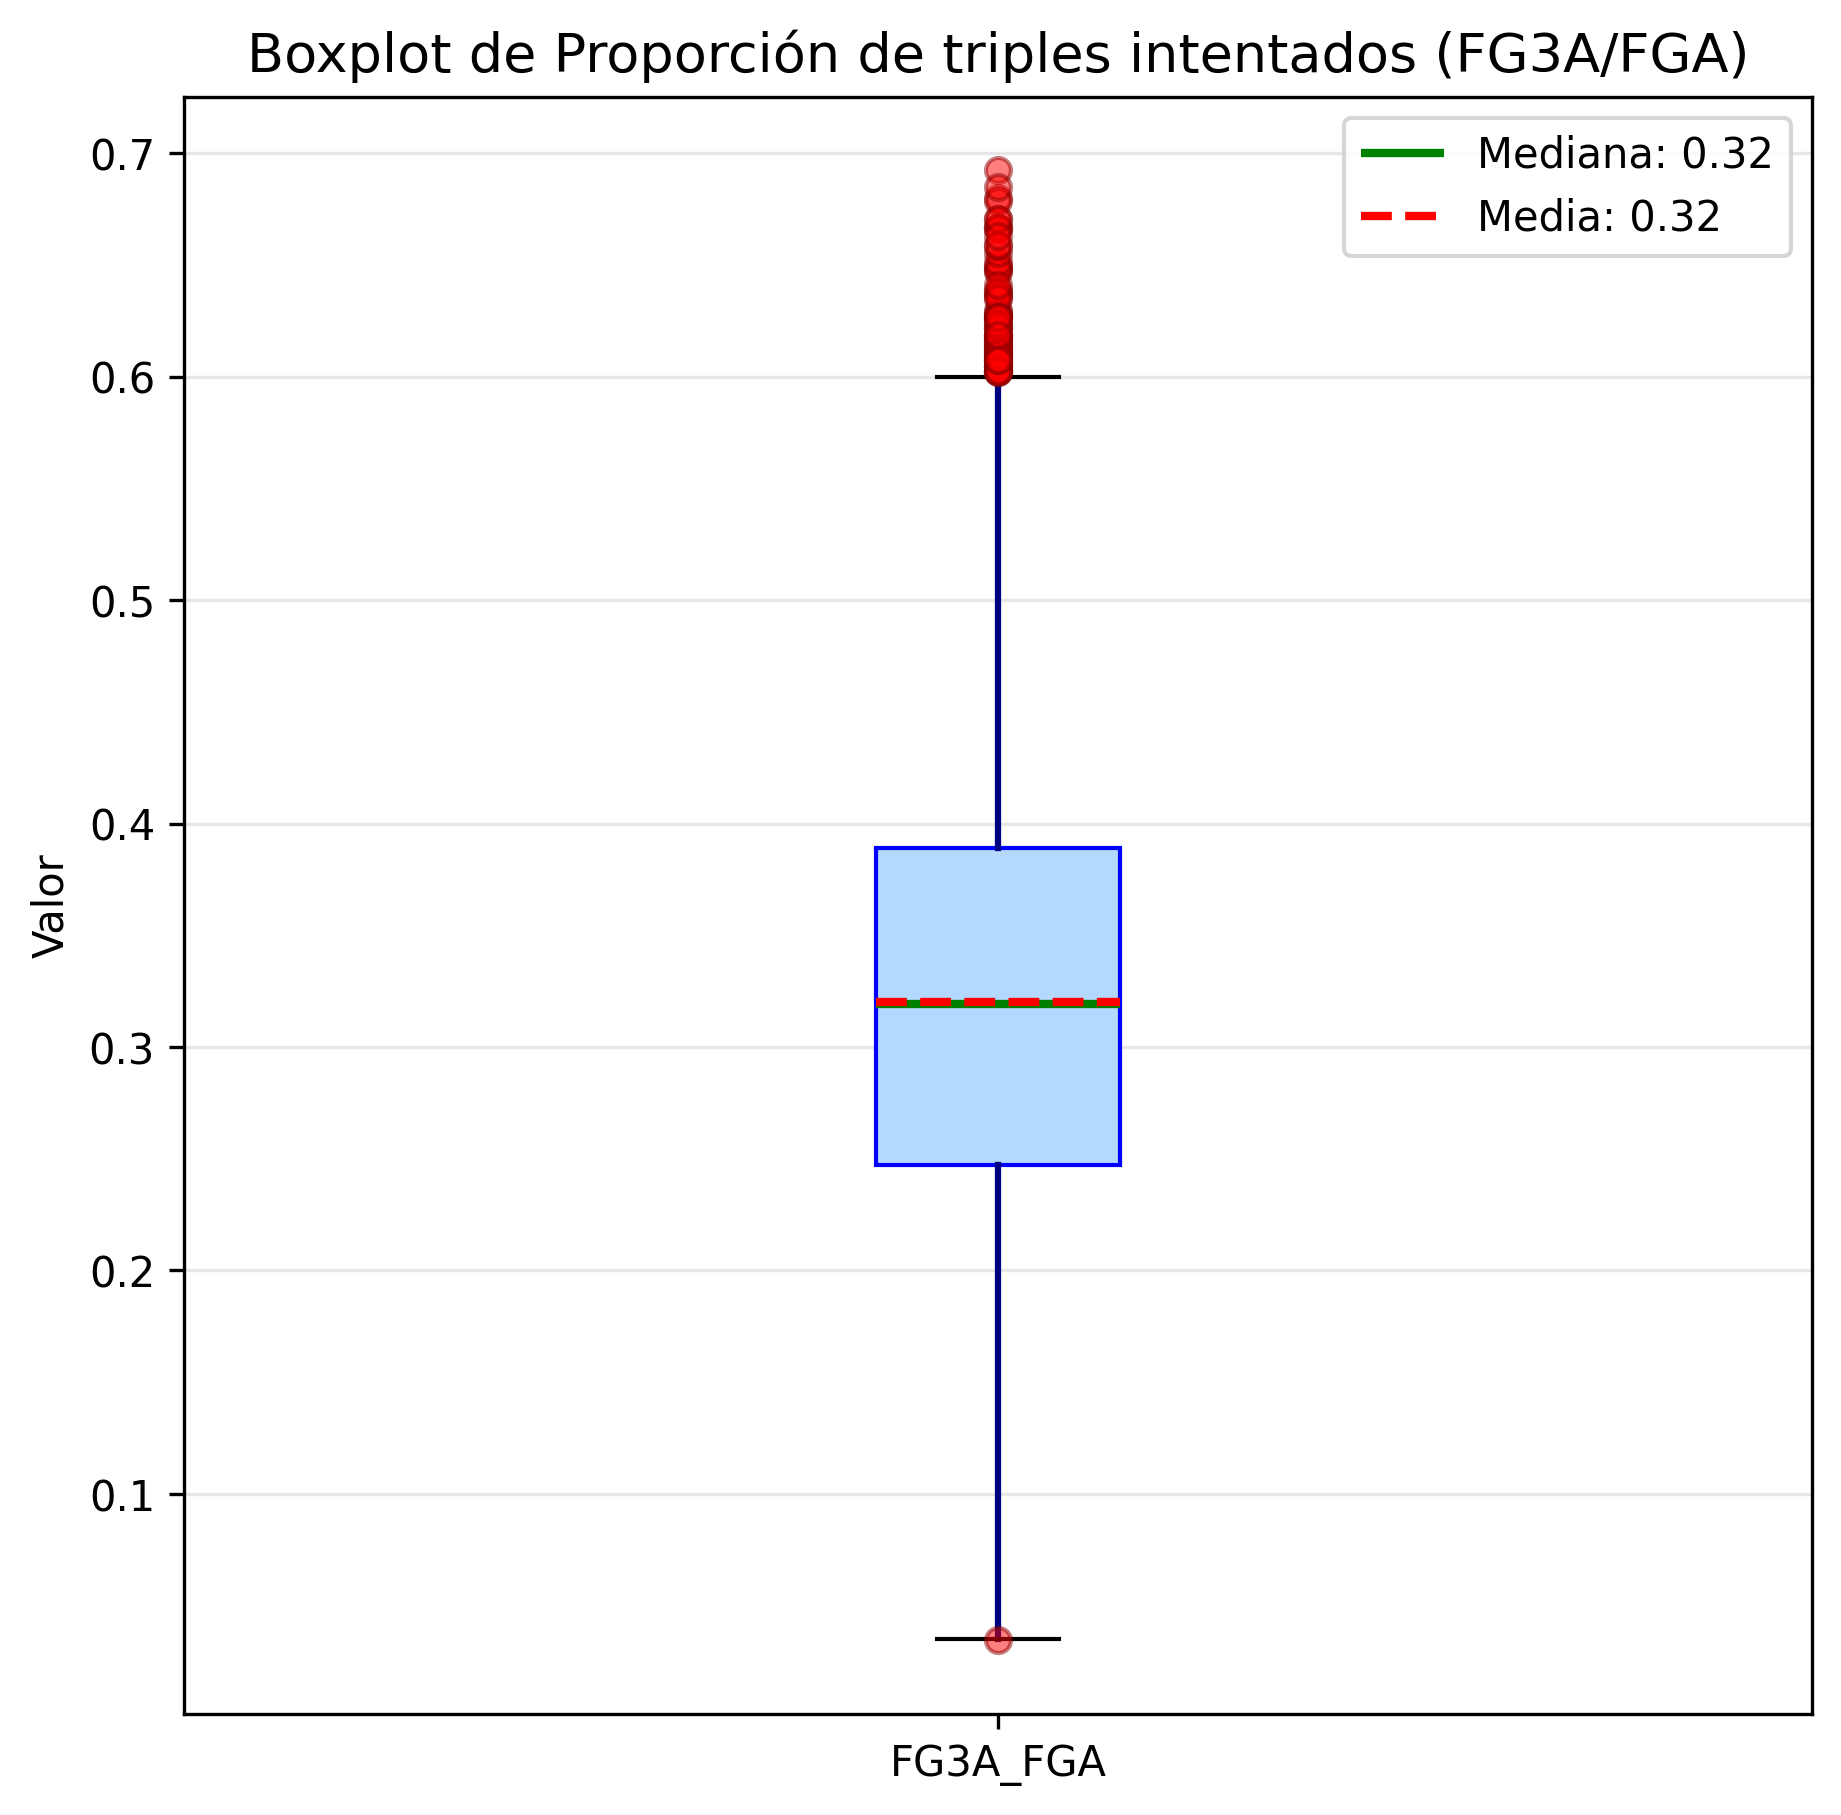
\includegraphics[width=\textwidth]{images/boxplots/boxplot_FG3A_FGA.png}
        \caption{FG3A/FGA}
        \label{fig:FG3A_FGA_eff}
    \end{subfigure}
    
    \caption{Boxplots de las métricas de eficiencia y perfil de tiro.}
    \label{fig:boxplots_efficiency}
\end{figure}

\subsubsection*{Boxplot del Diferencial de Puntos (PLUS\_MINUS)}

El boxplot de PLUS\_MINUS se caracteriza por una perfecta simetría alrededor de cero, con
mediana y media coincidentes y un rango intercuartílico amplio (IQR = 18). Este comportamiento
es consistente con un conjunto de datos balanceado que incluye tanto victorias como derrotas.
La presencia de numerosos valores atípicos en ambos extremos refleja partidos con diferencias
marcadas en el marcador, representativos de contextos competitivos desiguales o rendimientos
excepcionales.

\begin{figure}[H]
    \centering
    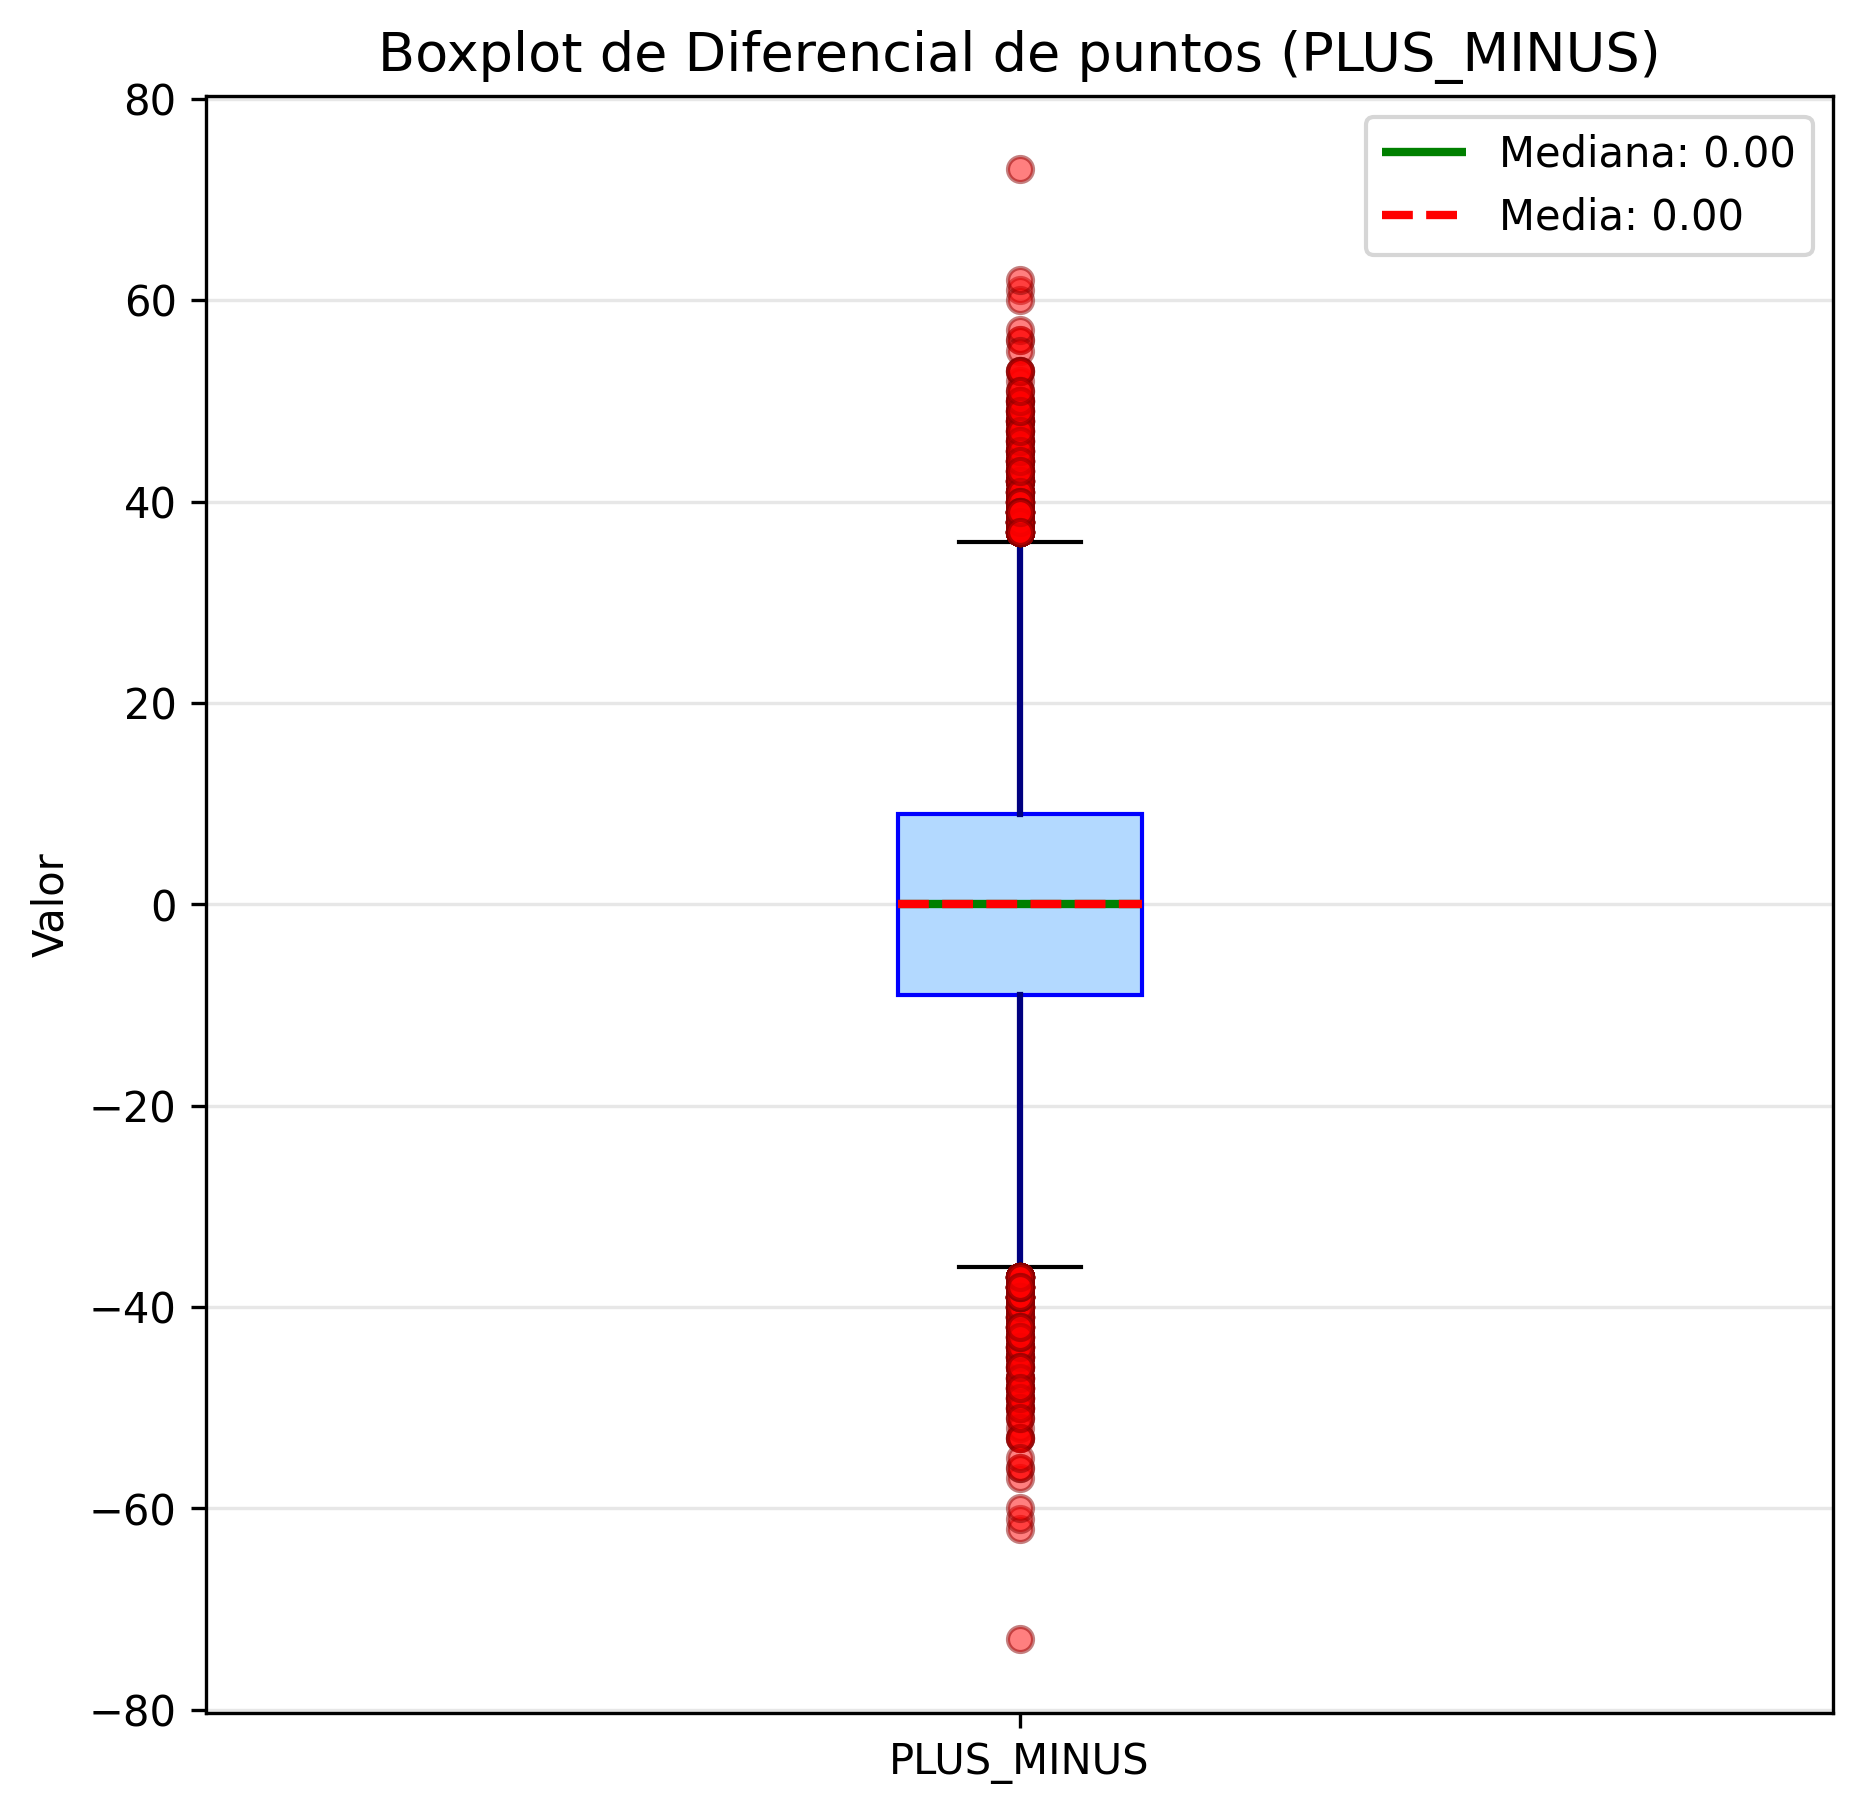
\includegraphics[width=0.5\textwidth]{images/boxplots/boxplot_PLUS_MINUS.png}
    \caption{Boxplot del diferencial de puntos (PLUS\_MINUS).}
    \label{fig:boxplot_plus_minus}
\end{figure}

\subsubsection*{Boxplot de los Robos de Balón (STL)}

La variable STL exhibe un boxplot claramente asimétrico hacia la derecha, con mediana de 7 robos
y un rango intercuartílico reducido (IQR = 3). La elevada cantidad de valores atípicos superiores
indica la existencia de partidos con presión defensiva intensa y alta capacidad de recuperación
de balón. Esta asimetría es característica de variables de conteo con límite inferior en cero y
confirma que los robos representan eventos menos frecuentes pero altamente dependientes del
contexto defensivo y del rival.

\begin{figure}[H]
    \centering
    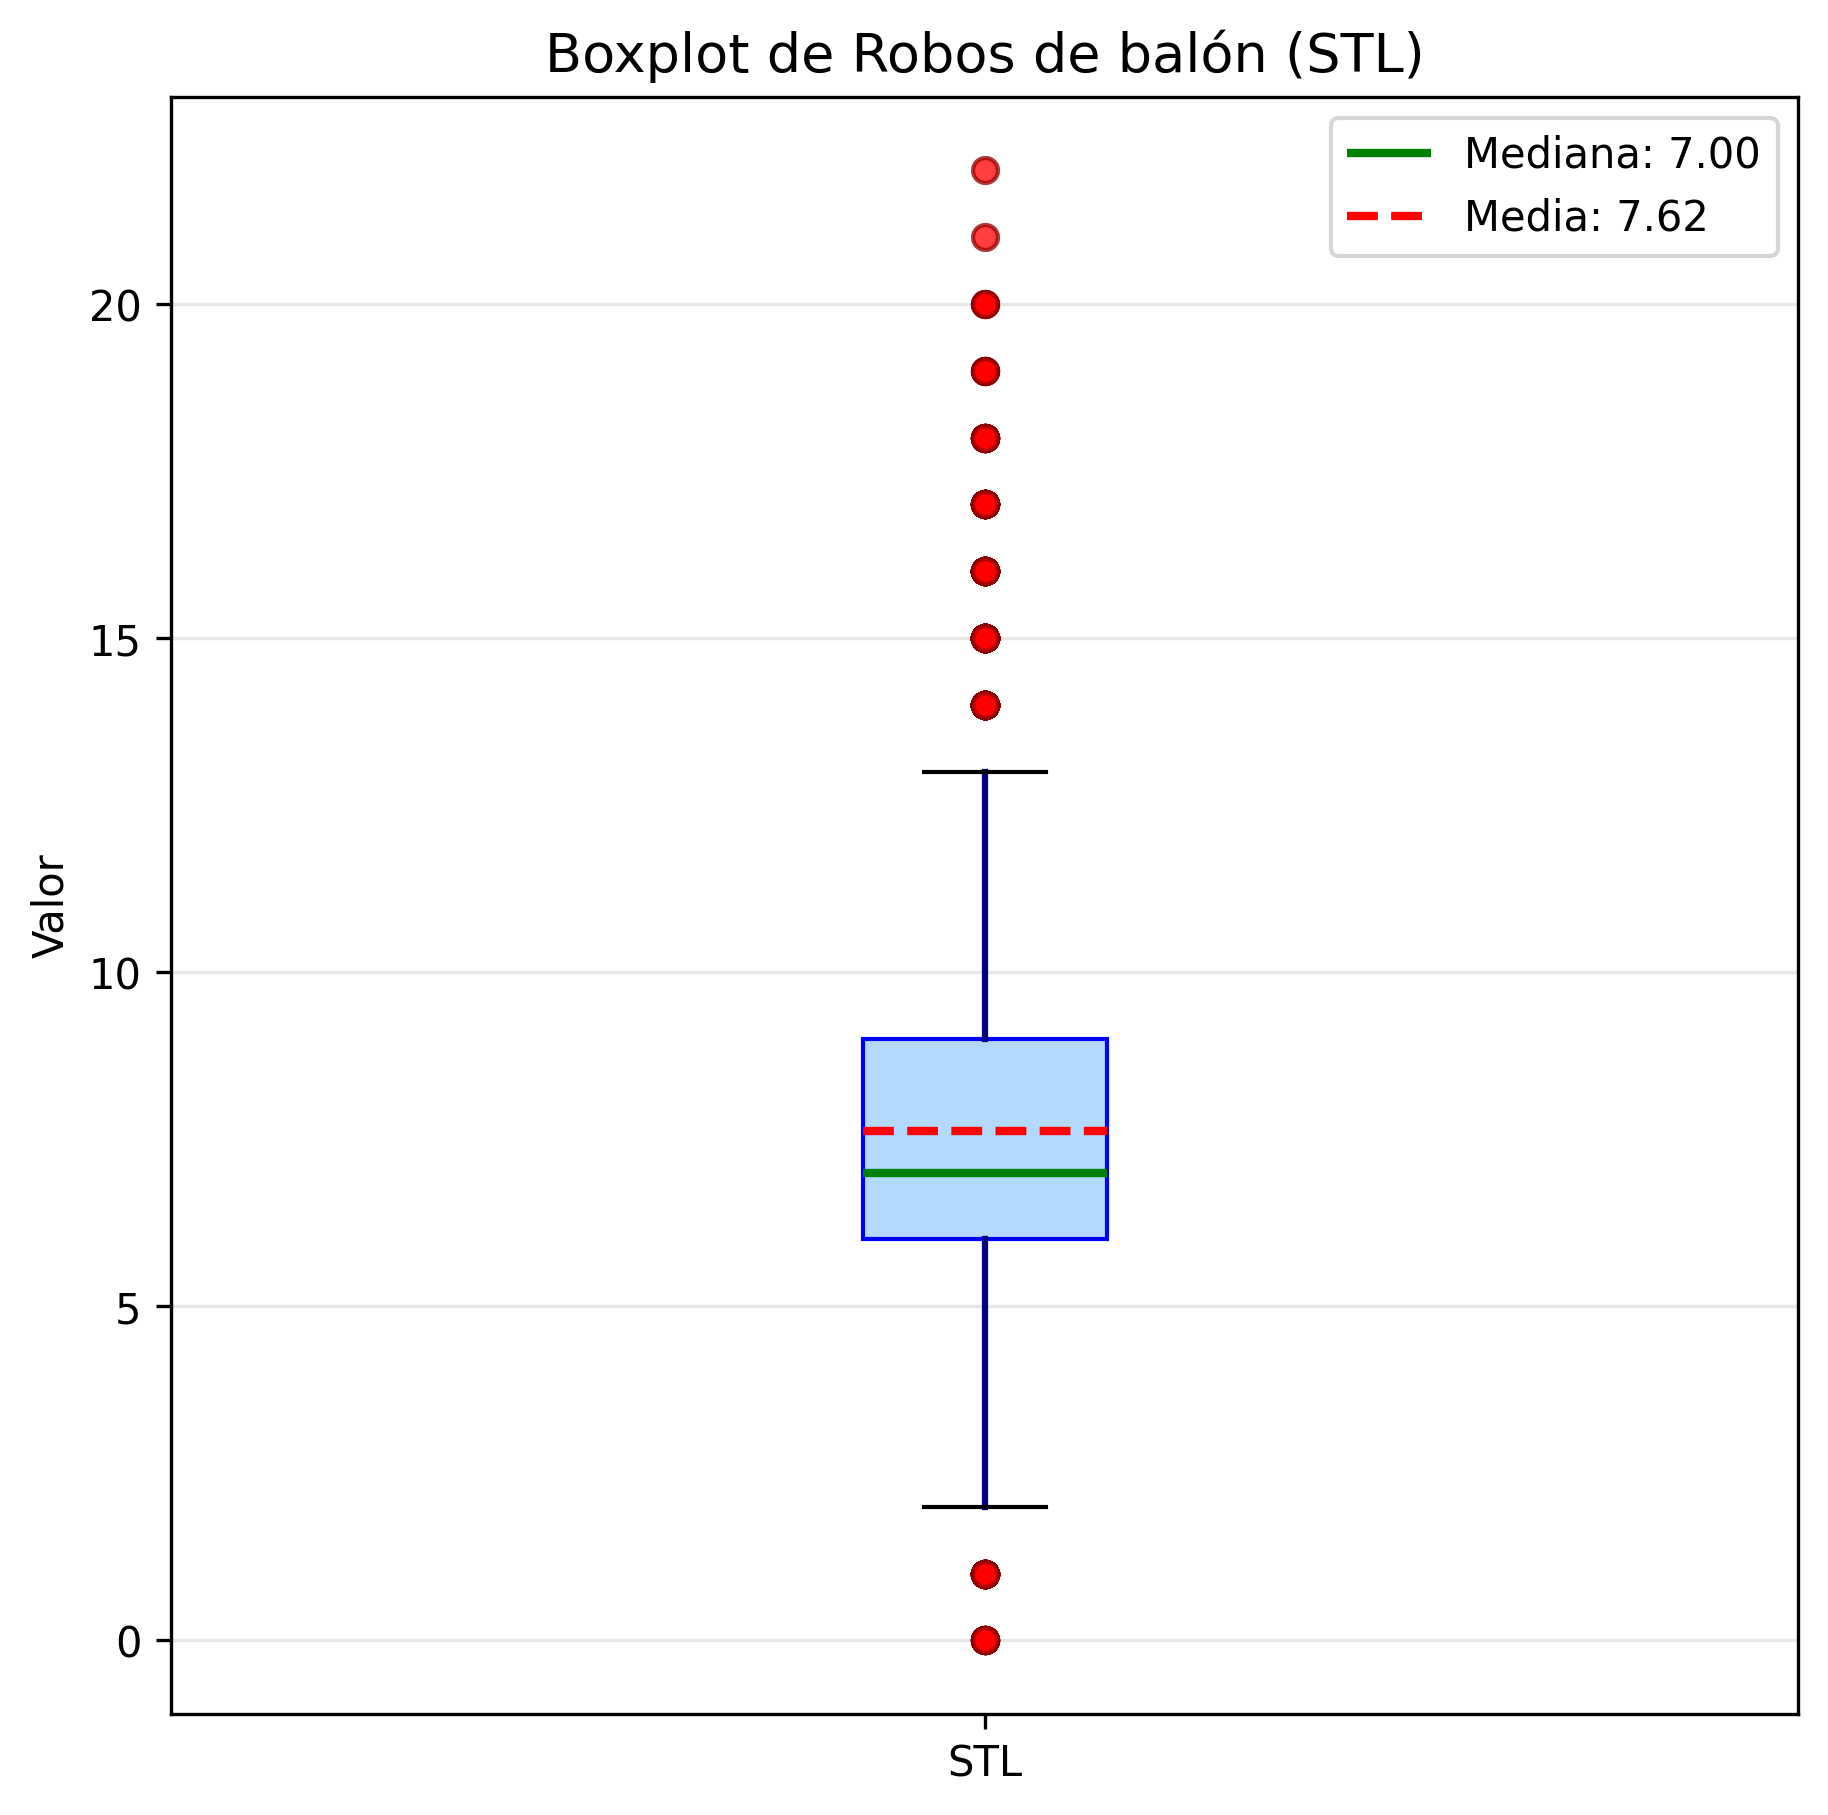
\includegraphics[width=0.5\textwidth]{images/boxplots/boxplot_STL.png}
    \caption{Boxplot de los robos de balón (STL).}
    \label{fig:boxplot_stl}
\end{figure}

\subsubsection*{Boxplot de los Bloqueos (BLK)}

El boxplot de BLK muestra una mediana de 5 bloqueos por partido y un rango intercuartílico de 3,
con una distribución también asimétrica hacia la derecha. La proximidad entre media y mediana
sugiere un equilibrio razonable en la estructura central, aunque la presencia de numerosos
valores atípicos elevados refleja partidos con una actividad defensiva excepcional cerca del
aro. Este comportamiento confirma que los bloqueos, al igual que los robos, son eventos
discretos y situacionales, sensibles a la composición del equipo y al tipo de ataque rival.

\begin{figure}[H]
    \centering
    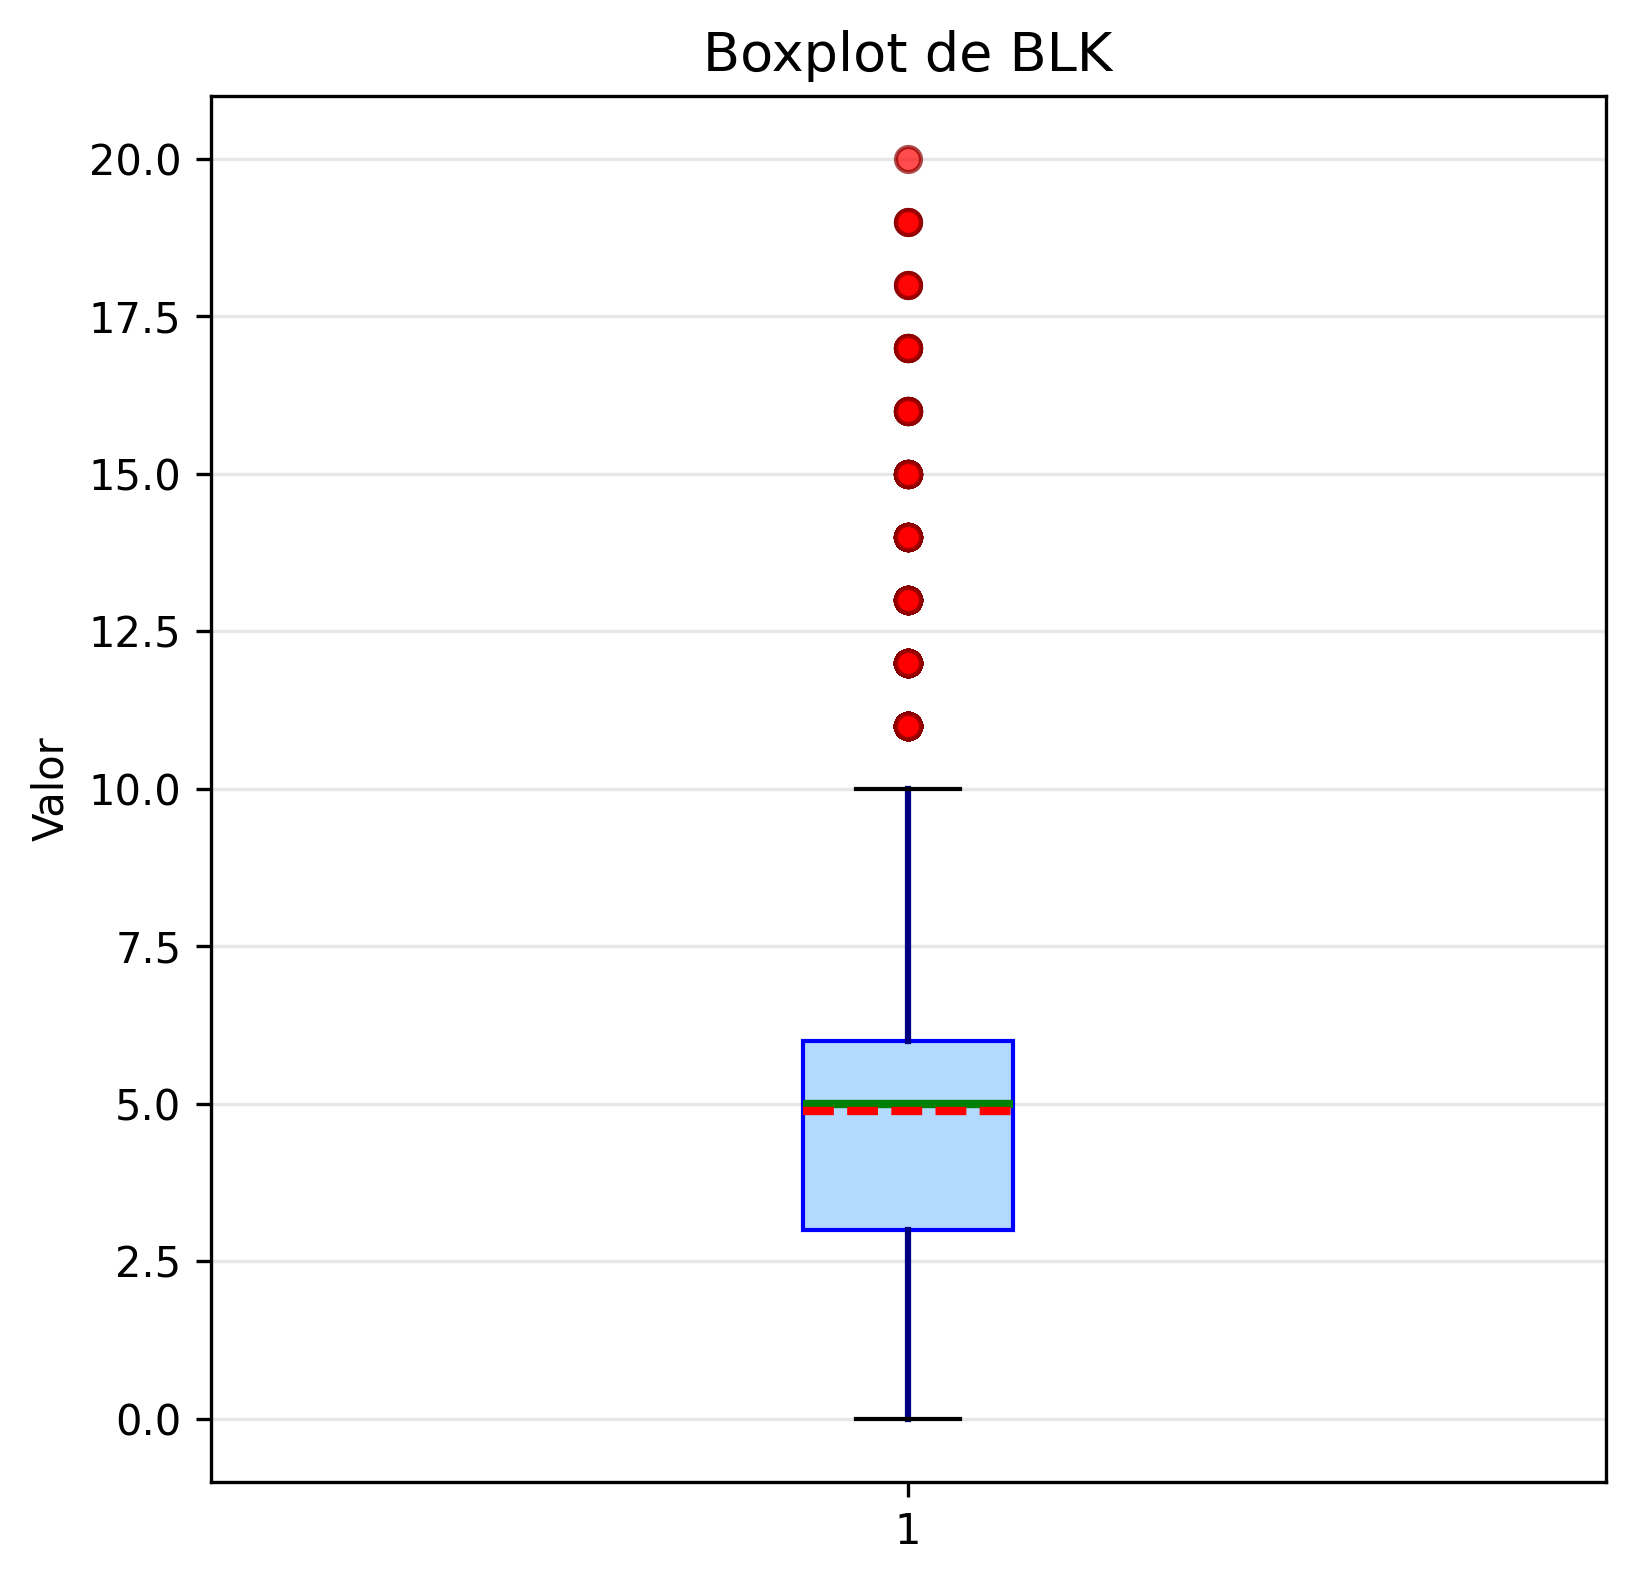
\includegraphics[width=0.5\textwidth]{images/boxplots/boxplot_BLK.png}
    \caption{Boxplot de los bloqueos (BLK).}
    \label{fig:boxplot_blk}
\end{figure}

\section{Pregunta 1: Análisis de la Relación entre Triples y Victoria}
\label{subsec:pregunta1-analisis}

\vspace{0.3cm}
¿Existe una correlación significativa entre el número de triples anotados (FG3M) y la victoria (WL) de un equipo en un partido, controlando por la efectividad general de tiro (FG\_PCT)?


Con el objetivo de responder de forma robusta a la Pregunta 1, se adoptó un enfoque
estadístico complementario que combina un modelo de regresión logística binaria
con una prueba no paramétrica de comparación de grupos Mann--Whitney U. 
Esta estrategia permite evaluar la relación entre el
número de triples anotados y la probabilidad de victoria desde dos perspectivas
estadísticas coherentes pero conceptualmente distintas.


\subsection{Regresión logística binaria}

La regresión logística se emplea como herramienta principal de modelación, dado que la
variable respuesta es dicotómica (WL: victoria/derrota). Este modelo permite
cuantificar el efecto marginal del número de triples anotados (FG3M) sobre la
probabilidad de ganar un partido, controlando simultáneamente por la efectividad general
de tiro (FG\_PCT). En este contexto, el objetivo de la regresión logística es
evaluar si el volumen de triples posee un impacto estadísticamente significativo sobre la
probabilidad de victoria, independientemente de la eficiencia ofensiva global, expresando
los resultados en términos de odds ratios, fácilmente interpretables en el ámbito
deportivo.


Previo a la estimación del modelo de regresión logística binaria, se realizó una
preparación y exploración de las variables con el objetivo de garantizar la
validez estadística del análisis y justificar la metodología empleada.

La variable respuesta fue codificada de forma binaria como
WL\_bin, donde $1$ representa victoria y $0$ derrota, lo cual es
coherente con la naturaleza dicotómica requerida por la regresión logística.
Como variables predictoras se utilizaron el número de triples anotados
(FG3M) y el porcentaje total de tiros de campo convertidos
(FG\_PCT), seleccionadas por su relevancia directa en la producción
ofensiva y su vínculo teórico con la probabilidad de victoria.


El análisis se planteó bajo las siguientes hipótesis inferenciales:

\begin{itemize}
    \item Hipótesis principal del modelo logístico:
    \[
    H_0: \beta_{\text{FG3M}} = 0 \quad \text{vs.} \quad H_1: \beta_{\text{FG3M}} \neq 0
    \]
    lo que implica contrastar si el número de triples anotados tiene un efecto
    estadísticamente significativo sobre la probabilidad de victoria,
    controlando por la efectividad general de tiro.

    \item Hipótesis auxiliar:
    \[
    H_0: \beta_{\text{FG\_PCT}} = 0 \quad \text{vs.} \quad H_1: \beta_{\text{FG\_PCT}} \neq 0
    \]
    evaluando el impacto de la eficiencia ofensiva total en el resultado del
    partido.
\end{itemize}

Cada observación del conjunto de datos corresponde a un partido distinto,
por lo que se asume independencia entre observaciones. Este supuesto se
considera satisfecho por el propio diseño del experimento observacional,
al no existir mediciones repetidas ni dependencia temporal directa entre filas.


A diferencia de los modelos lineales clásicos, la regresión logística no
requiere normalidad de las variables explicativas ni homocedasticidad de los
residuos, ya que la variable respuesta sigue una distribución binomial y el
modelo se estima mediante máxima verosimilitud. En consecuencia, la ausencia
de normalidad en variables como FG3M no invalida el uso de este modelo.

\subsubsection{Evaluación de supuestos y resultados del modelo logístico}
La correlación de Spearman entre FG3M y FG\_PCT fue $\rho = 0.280$ con un valor-p de $p = 0.0000$.

\begin{table}[H]
\centering
\caption{Factores de Inflación de la Varianza (VIF)}
\label{tab:vif}
\begin{tabular}{lr}
\toprule
Variable & VIF \\
\midrule
const & 69.646 \\
FG3M & 1.096 \\
FG\_PCT & 1.096 \\
\bottomrule
\end{tabular}
\end{table}


\begin{table}[H]
\centering
\caption{Coeficientes del modelo Logit}
\label{tab:logit_coef}
\begin{tabular}{lrrrr}
\toprule
 & Coeficiente & Std.Error & z & p-value \\
\midrule
const & -9.4013 & 0.1272 & -73.9209 & 0.0000 \\
FG3M & 0.0496 & 0.0031 & 16.1441 & 0.0000 \\
FG\_PCT & 19.3723 & 0.2787 & 69.5131 & 0.0000 \\
\bottomrule
\end{tabular}
\end{table}


\begin{table}[H]
\centering
\caption{Odds Ratios e intervalos de confianza al 95\%}
\label{tab:odds_ratios}
\begin{tabular}{lrrr}
\toprule
 & OR & CI 2.5\textbackslash \% & CI 97.5\textbackslash \% \\
\midrule
const & 0.0001 & 0.0001 & 0.0001 \\
FG3M & 1.0508 & 1.0445 & 1.0572 \\
FG\_PCT & 258998289.0146 & 149995784.2750 & 447213326.9393 \\
\bottomrule
\end{tabular}
\end{table}


\begin{table}[H]
\centering
\caption{Métricas de ajuste del modelo}
\label{tab:metricas}
\begin{tabular}{lr}
\toprule
Métrica & Valor \\
\midrule
Pseudo \$R\textasciicircum 2\$ (McFadden) & 0.1683 \\
Log-Likelihood & -19206.1154 \\
AIC & 38418.2308 \\
N Observaciones & 33316.0000 \\
\bottomrule
\end{tabular}
\end{table}


Antes de estimar el modelo de regresión logística, se evaluó la posible dependencia
entre las variables explicativas con el objetivo de descartar problemas de
multicolinealidad. Para ello, se calculó la correlación de Spearman entre
\texttt{FG3M} y \texttt{FG\_PCT}, obteniéndose un coeficiente
$\rho = 0.280$ con un valor-p $p < 0.001$. Este resultado indica la existencia de
una asociación positiva de magnitud moderada, lo cual sugiere que ambas variables
están relacionadas, pero no de forma lo suficientemente intensa como para generar
inestabilidad en la estimación de los parámetros del modelo.

Este diagnóstico se confirma mediante los Factores de Inflación de la Varianza
(VIF), presentados en la Tabla~\ref{tab:vif}. Los valores de VIF para
\texttt{FG3M} y \texttt{FG\_PCT} son cercanos a 1, muy por debajo de los umbrales
habitualmente utilizados para identificar multicolinealidad problemática
(VIF $> 5$ o $> 10$). En consecuencia, se concluye que ambas variables pueden ser
incluidas simultáneamente en el modelo sin comprometer la estabilidad ni la
interpretabilidad de los coeficientes estimados.

Una vez verificados los supuestos estructurales básicos, se procedió a la
estimación del modelo de regresión logística binaria. Los coeficientes estimados,
sus errores estándar y niveles de significación se presentan en la
Tabla~\ref{tab:logit_coef}. El modelo converge correctamente, lo que indica
estabilidad en el proceso de maximización de la verosimilitud.

Los resultados muestran que ambas variables explicativas tienen un efecto positivo
y estadísticamente significativo sobre la probabilidad de victoria. En particular,
el coeficiente asociado a \texttt{FG3M} es positivo
($\hat{\beta} = 0.0496$, $p < 0.001$), lo que implica que, manteniendo constante la
efectividad de tiro, un aumento en el número de triples anotados incrementa la
probabilidad de ganar el partido. De forma análoga, \texttt{FG\_PCT} presenta un
coeficiente positivo de gran magnitud
($\hat{\beta} = 19.37$, $p < 0.001$), reflejando el papel central de la eficiencia
ofensiva en el resultado final del encuentro.

Para facilitar la interpretación de estos efectos, la Tabla~\ref{tab:odds_ratios}
presenta los correspondientes \emph{odds ratios}. En este contexto, un incremento
unitario en \texttt{FG3M} multiplica las probabilidades de victoria por un factor
aproximado de 1.05, mientras que aumentos en \texttt{FG\_PCT} se asocian con un
crecimiento muy pronunciado de las probabilidades de éxito, coherente con la fuerte
influencia de la eficiencia de tiro observada en los coeficientes del modelo.

Finalmente, la calidad global del ajuste se resume en la
Tabla~\ref{tab:metricas}. El pseudo coeficiente de determinación de McFadden
($R^2 = 0.168$) indica que el modelo explica una proporción relevante de la
variabilidad del resultado del partido, especialmente considerando la naturaleza
binaria del fenómeno analizado. Asimismo, los valores del log-verosímil y del
criterio de información de Akaike (AIC) respaldan la adecuación del modelo como una
representación parsimoniosa y estadísticamente sólida de la relación entre el
rendimiento en tiros de tres puntos y la probabilidad de victoria.

\vspace{0.3cm}
En conjunto, los resultados del análisis evidencian que el número de triples anotados tiene un efecto positivo y estadísticamente significativo sobre la probabilidad de victoria, incluso al controlar por la efectividad general de tiro. La magnitud y significación de los coeficientes estimados confirman que tanto el volumen de anotación desde la línea de tres puntos como la eficiencia ofensiva contribuyen de forma independiente al éxito del equipo. Asimismo, los diagnósticos de multicolinealidad indican que ambas variables aportan información complementaria, permitiendo concluir que el incremento en triples convertidos aumenta la probabilidad de ganar un partido más allá del efecto explicado únicamente por la precisión en el tiro.

\subsection{Prueba de Mann--Whitney U para el número de triples anotados (FG3M)}

Como complemento al análisis multivariado basado en regresión logística, se aplicó la
prueba no paramétrica de Mann--Whitney U con el objetivo de comparar la distribución del
número de triples anotados (FG3M) entre partidos ganados y partidos perdidos. Esta prueba
permite evaluar si existen diferencias sistemáticas en el volumen de triples entre ambos
grupos sin asumir normalidad ni homocedasticidad, condiciones que no se cumplen para esta
variable según el análisis exploratorio previo.

La utilización de esta prueba resulta especialmente adecuada en este contexto debido al
carácter discreto de la variable FG3M y a la presencia de asimetrías y valores extremos,
frecuentes en estadísticas de rendimiento deportivo. 
    A diferencia de las pruebas paramétricas (como la prueba t de Student), la prueba de
    Mann--Whitney no requiere que la variable analizada siga una distribución normal ni
    que las varianzas de ambos grupos sean iguales.
En este sentido, la prueba aporta
una comparación robusta entre grupos y complementa los resultados obtenidos mediante la
regresión logística, al ofrecer evidencia directa sobre las diferencias observadas en los
datos sin imponer restricciones paramétricas.

En consecuencia, el diseño del estudio y la naturaleza de los datos garantizan el
cumplimiento de los supuestos necesarios para la aplicación de la prueba de
Mann--Whitney U. La independencia entre observaciones, la adecuada escala de medición de
FG3M y la independencia entre los grupos de partidos ganados y perdidos permiten interpretar
los resultados de la prueba con validez estadística, asegurando que las conclusiones
derivadas reflejan diferencias reales en la distribución del número de triples anotados.

\subsubsection{Preparación de los datos}
Antes de la realización de la prueba se seleccionaron únicamente las observaciones con
información válida en las variables \textit{WL} (resultado del partido) y \textit{FG3M}
(triples anotados). Posteriormente, los partidos se dividieron en dos grupos independientes:
victorias (\textit{WL = W}) y derrotas (\textit{WL = L}). Ambos grupos presentan tamaños
muestrales idénticos ($N = 16\,658$), lo que refuerza la robustez de la comparación.

El análisis exploratorio previo, mediante histogramas y boxplots, evidenció que la
distribución de FG3M es asimétrica, presenta colas largas y valores atípicos, lo que
invalida los supuestos de normalidad y homocedasticidad necesarios para pruebas
paramétricas. Por tanto, la elección de una prueba no paramétrica resulta adecuada y
metodológicamente justificada.

La variable FG3M es una variable discreta de conteo, con distribución asimétrica y presencia
de valores atípicos, características que justifican el uso de una prueba no paramétrica
basada en rangos en lugar de pruebas paramétricas como la t de Student.

\subsubsection{Hipótesis planteadas}

La prueba de Mann--Whitney U se utilizó para contrastar las siguientes hipótesis:

\begin{itemize}
    \item $H_0$: La distribución del número de triples anotados (FG3M) es la misma en partidos
    ganados y partidos perdidos.
    \item $H_1$: La distribución del número de triples anotados (FG3M) difiere entre partidos
    ganados y partidos perdidos.
\end{itemize}

Desde una perspectiva sustantiva, la hipótesis alternativa implica que los partidos ganados
tienden a presentar valores sistemáticamente mayores de triples anotados que los partidos
perdidos.

\subsubsection{Resultados e interpretación}

\begin{table}[H]
\centering
\caption{Estadísticos descriptivos de FG3M por resultado del partido}
\label{tab:fg3m_descriptivos}
\begin{tabular}{lrrrr}
\toprule
Grupo & N & Mediana FG3M & Q1 & Q3 \\
\midrule
Victorias & 16658 & 10.000 & 8.000 & 14.000 \\
Derrotas & 16658 & 9.000 & 6.000 & 12.000 \\
\bottomrule
\end{tabular}
\end{table}

\begin{table}[H]
\centering
\caption{Resultados de la prueba de Mann--Whitney U para FG3M}
\label{tab:mann_whitney_fg3m}
\begin{tabular}{rrrr}
\toprule
U statistic & Z value & p value & Effect size r \\
\midrule
170661761.0000 & 36.3631 & 0.0000 & 0.1992 \\
\bottomrule
\end{tabular}
\end{table}


Los estadísticos descriptivos presentados en la Tabla~\ref{tab:fg3m_descriptivos} muestran que la
mediana de triples anotados en los partidos ganados (Mediana = 10) es superior a la observada
en los partidos perdidos (Mediana = 9). Asimismo, los cuartiles primero y tercero del grupo de
victorias (Q1 = 8, Q3 = 14) se encuentran sistemáticamente desplazados hacia valores mayores en
comparación con los correspondientes al grupo de derrotas (Q1 = 6, Q3 = 12). Esta diferencia
en la localización y dispersión de las distribuciones sugiere, desde un punto de vista
descriptivo, una mayor producción de triples en los encuentros que culminan en victoria.

Desde el enfoque inferencial, los resultados de la prueba de Mann--Whitney U, resumidos en la
Tabla~\ref{tab:mann_whitney_fg3m}, indican un estadístico $U = 170,661,761$, con un valor
estandarizado $Z = 36.36$ y un \textit{p-value} inferior a 0.001. Este resultado proporciona
evidencia estadística muy sólida para rechazar la hipótesis nula de igualdad entre las
distribuciones de FG3M en partidos ganados y perdidos, confirmando que la diferencia observada
no puede atribuirse al azar.

Adicionalmente, el tamaño del efecto estimado ($r = 0.199$) corresponde a un efecto pequeño a
moderado según los criterios habituales. Este valor indica que, aunque la diferencia entre
ambos grupos es altamente significativa desde el punto de vista estadístico —favorecida en
parte por el gran tamaño muestral—, el número de triples anotados explica únicamente una
proporción limitada, aunque relevante, de la variabilidad asociada al resultado del partido.

\subsubsection{Conclusión de la prueba}

En conjunto, los resultados de la prueba de Mann--Whitney U confirman que los partidos ganados
tienden a presentar un mayor número de triples anotados que los partidos perdidos. Esta
evidencia inferencial, basada en una comparación directa de las distribuciones de FG3M entre
ambos grupos, complementa los hallazgos obtenidos mediante la regresión logística y refuerza la
idea de que el tiro de tres puntos constituye un factor relevante en la probabilidad de
victoria, aunque no exclusivo ni suficiente por sí solo para explicar el resultado de un
partido.

\subsection*{Conclusión global del análisis}

Los resultados obtenidos mediante la regresión logística y la prueba no paramétrica de
Mann--Whitney U son consistentes y complementarios. El análisis multivariado muestra que el
número de triples anotados (FG3M) se asocia de forma positiva y estadísticamente significativa
con la probabilidad de victoria, incluso al controlar por la efectividad general de tiro
(FG\_PCT), lo que confirma la relevancia independiente del lanzamiento de tres puntos en el
resultado del partido.

De manera concordante, la prueba de Mann--Whitney U evidencia que los equipos ganadores
presentan, en términos generales, un mayor volumen de triples anotados que los equipos
perdedores, con una diferencia altamente significativa desde el punto de vista estadístico,
aunque de magnitud moderada. En conjunto, ambos enfoques refuerzan la conclusión de que el tiro
de tres puntos constituye un factor relevante en la probabilidad de victoria, si bien su
efecto debe interpretarse como parte de un conjunto más amplio de determinantes del
rendimiento competitivo.



\section{Pregunta 2: Análisis de la Evolución Temporal del Juego}
\label{subsec:pregunta2-analisis}

\vspace{0.3cm}

¿Como ha cambiado la media de puntos por partido (PTS) y el porcentaje de tiros de tres puntos intentados (FG3A/FGA) a lo largo de las temporadas (SEASON\_YEAR), y existe una relación temporal significativa entre ambas variables?

\vspace{0.3cm}

Para estudiar la evolución temporal de la producción ofensiva se combinaron dos enfoques
estadísticos complementarios: un análisis de varianza (ANOVA) de una vía y un modelo de
regresión lineal. Esta estrategia permite responder a la pregunta desde una perspectiva
comparativa y desde una perspectiva temporal continua.

El ANOVA de una vía se utilizó para evaluar si las medias de puntos por partido (PTS) y del
porcentaje de tiros de tres puntos intentados (FG3A/FGA) difieren significativamente entre
temporadas. Este análisis permite detectar la existencia de cambios estructurales en el
promedio de estas variables a lo largo del tiempo, sin asumir una forma funcional específica
para dicha evolución.

Sin embargo, el ANOVA no proporciona información sobre la dirección ni la magnitud del cambio
temporal. Por esta razón, se estimaron modelos de regresión lineal utilizando la temporada
como variable explicativa continua. Este enfoque permite evaluar si existe una tendencia
temporal sistemática, determinar si el cambio es creciente o decreciente y cuantificar la
tasa media de variación anual de cada indicador ofensivo.

En conjunto, el ANOVA permite identificar diferencias significativas entre temporadas, mientras
que la regresión lineal traduce estas diferencias en una relación temporal interpretable,
ofreciendo una visión integral de cómo ha evolucionado el juego y de si ambas variables
presentan una dinámica temporal significativa y coherente.

\subsection{Ejecución de ANOVA}

En primer lugar, se aplicó un ANOVA de una vía con el objetivo de evaluar si las medias
de las variables de interés difieren de forma estadísticamente significativa entre
temporadas. En este contexto, la temporada actúa como un factor categórico que divide el
conjunto de datos en múltiples grupos independientes, mientras que las variables respuesta
(PTS y FG3A/FGA) son cuantitativas continuas. El ANOVA resulta apropiado cuando se desea
comparar medias entre más de dos grupos, evitando la realización de múltiples contrastes
bivariados que incrementarían el riesgo de error tipo I.

La aplicación del ANOVA está respaldada por el análisis exploratorio previo. Los boxplots y
estadísticos descriptivos mostraron que, a nivel agregado por temporada, las distribuciones
de PTS y FG3A/FGA presentan rangos intercuartílicos moderados y una variabilidad relativamente
estable entre temporadas. Además, el elevado tamaño muestral por grupo permite invocar el
teorema del límite central, de modo que las medias muestrales pueden considerarse
aproximadamente normales, aun cuando los datos a nivel de partido no sigan estrictamente una
distribución normal. Esta característica confiere robustez al ANOVA frente a desviaciones
moderadas de normalidad.

\paragraph{Homoscedasticidad}

El supuesto de homogeneidad de varianzas implica que la dispersión de la variable respuesta
sea comparable entre temporadas. La inspección gráfica mediante boxplots por temporada
mostró rangos intercuartílicos relativamente estables, sin evidencia de varianzas
extremadamente desiguales entre grupos.

Si bien pueden existir diferencias leves en la variabilidad entre temporadas, estas no son
suficientemente pronunciadas como para invalidar el ANOVA, el cual es conocido por su
robustez ante heterocedasticidad moderada cuando los tamaños muestrales son grandes y
balanceados.


\subsubsection{Preparación de los datos}
\label{subsubsec:anova-preparacion-supuestos}

Para aplicar un ANOVA de una vía en el análisis de la evolución temporal, fue necesaria una
preparación previa de los datos y la evaluación de los supuestos asociados a esta técnica.


En primer lugar, la variable temporal SEASON\_YEAR se trató como un factor categórico,
dado que el objetivo del ANOVA es comparar las medias de las variables de interés entre
temporadas discretas. Cada nivel del factor representa una temporada de la NBA, lo que
define grupos independientes de observaciones.

Las variables respuesta consideradas fueron:

\begin{itemize}
    \item PTS: puntos totales anotados por partido.
    \item FG3A/FGA: proporción de intentos de triple sobre el total de tiros de campo.
\end{itemize}

Para la variable FG3A/FGA, se construyó explícitamente la razón entre FG3A y FGA a nivel de
partido, garantizando que ambas variables estuvieran definidas y fueran positivas. Esta
transformación permite capturar la orientación estratégica hacia el tiro de tres puntos de
forma estandarizada y comparable entre temporadas.

Posteriormente, se eliminaron observaciones con valores faltantes en cualquiera de las
variables implicadas, asegurando la consistencia del conjunto de datos utilizado en el
análisis.

\subsection{Hipótesis estadísticas}

Para cada variable dependiente se plantearon las siguientes hipótesis:

\paragraph{Para FG3A/FGA}
\begin{itemize}
    \item $H_0$: La media de FG3A/FGA es igual en todas las temporadas.
    \item $H_1$: Al menos una temporada presenta una media de FG3A/FGA diferente.
\end{itemize}

\paragraph{Para PTS}
\begin{itemize}
    \item $H_0$: La media de puntos por partido (PTS) es igual en todas las temporadas.
    \item $H_1$: Al menos una temporada presenta una media de PTS diferente.
\end{itemize}

\subsection{Resultados del ANOVA}

%\begin{table}
\caption{Estadísticos descriptivos de FG3A/FGA por temporada}
\label{tab:anova-desc-fg3}
\begin{tabular}{lrrr}
\toprule
 & mean & std & n \\
SEASON_YEAR &  &  &  \\
\midrule
2010-11 & 0.222 & 0.069 & 2460 \\
2011-12 & 0.226 & 0.071 & 1980 \\
2012-13 & 0.244 & 0.071 & 2458 \\
2013-14 & 0.260 & 0.071 & 2460 \\
2014-15 & 0.268 & 0.075 & 2460 \\
2015-16 & 0.285 & 0.077 & 2460 \\
2016-17 & 0.317 & 0.076 & 2460 \\
2017-18 & 0.338 & 0.077 & 2460 \\
2018-19 & 0.359 & 0.078 & 2460 \\
2019-20 & 0.384 & 0.076 & 2118 \\
2020-21 & 0.393 & 0.079 & 2160 \\
2021-22 & 0.400 & 0.073 & 2460 \\
2022-23 & 0.388 & 0.077 & 2460 \\
2023-24 & 0.395 & 0.068 & 2460 \\
\bottomrule
\end{tabular}
\end{table}


%\begin{table}
\caption{Estadísticos descriptivos de PTS por temporada}
\label{tab:anova-desc-pts}
\begin{tabular}{lrrr}
\toprule
 & mean & std & n \\
SEASON_YEAR &  &  &  \\
\midrule
2010-11 & 99.550 & 12.002 & 2460 \\
2011-12 & 96.260 & 11.635 & 1980 \\
2012-13 & 98.138 & 11.631 & 2458 \\
2013-14 & 101.009 & 11.861 & 2460 \\
2014-15 & 100.014 & 11.757 & 2460 \\
2015-16 & 102.672 & 11.741 & 2460 \\
2016-17 & 105.591 & 12.149 & 2460 \\
2017-18 & 106.333 & 12.065 & 2460 \\
2018-19 & 111.209 & 12.651 & 2460 \\
2019-20 & 111.798 & 12.436 & 2118 \\
2020-21 & 112.091 & 12.507 & 2160 \\
2021-22 & 110.616 & 12.620 & 2460 \\
2022-23 & 114.686 & 11.967 & 2460 \\
2023-24 & 114.211 & 12.846 & 2460 \\
\bottomrule
\end{tabular}
\end{table}


%\begin{table}
\caption{ANOVA de una vía para FG3A/FGA por temporada}
\label{tab:anova-fg3}
\begin{tabular}{lrrrr}
\toprule
 & sum_sq & df & F & PR(>F) \\
\midrule
C(SEASON_YEAR) & 139.5719 & 13.0000 & 1950.5527 & 0.0000 \\
Residual & 183.3020 & 33302.0000 & NaN & NaN \\
\bottomrule
\end{tabular}
\end{table}


%\begin{table}
\caption{ANOVA de una vía para PTS por temporada}
\label{tab:anova-pts}
\begin{tabular}{lrrrr}
\toprule
 & sum_sq & df & F & PR(>F) \\
\midrule
C(SEASON_YEAR) & 1241374.2803 & 13.0000 & 647.8556 & 0.0000 \\
Residual & 4908530.6579 & 33302.0000 & NaN & NaN \\
\bottomrule
\end{tabular}
\end{table}


Los resultados del ANOVA se presentan en las Tablas \ref{tab:anova-fg3} y \ref{tab:anova-pts}.

Para la variable FG3A/FGA, el estadístico F obtenido es $F = 1950.55$ con un valor-p prácticamente nulo ($p < 0.001$). Esto proporciona evidencia estadística muy fuerte para rechazar la hipótesis nula, indicando que la proporción de triples ha cambiado significativamente entre temporadas.

De manera análoga, para la variable PTS se obtuvo un estadístico $F = 647.86$ con $p < 0.001$, lo que indica diferencias estadísticamente significativas en la media de puntos por partido entre temporadas.

Estos resultados son coherentes con los estadísticos descriptivos, donde se observa un incremento progresivo tanto en la proporción de triples como en la cantidad de puntos anotados a lo largo del tiempo.


\subsection{Conclusión}

En conclusión, los resultados del ANOVA muestran evidencia estadística contundente de que tanto la proporción de lanzamientos de tres puntos como la cantidad de puntos anotados por partido han variado significativamente entre temporadas. A pesar de que los supuestos de normalidad y homocedasticidad no se cumplen estrictamente según las pruebas formales, el gran tamaño de la muestra y el balance entre grupos permiten considerar válidas las conclusiones obtenidas.

Estos hallazgos respaldan la idea de una evolución estructural del juego en la NBA, caracterizada por un aumento sostenido del uso del tiro de tres puntos y del ritmo ofensivo a lo largo del tiempo.



\subsection{Regresión lineal para el análisis temporal (Pregunta 2)}
\label{subsec:pregunta2-regresion}

Con el objetivo de cuantificar la evolución temporal observada en el análisis descriptivo y confirmada por el ANOVA, se aplicó un modelo de regresión lineal simple para evaluar la relación entre el tiempo (temporadas) y las variables de interés.

\subsubsection{Evaluación de los supuestos del modelo}

El modelo de regresión lineal se apoya en cuatro supuestos principales:

\paragraph{Linealidad}
La relación entre la variable temporal y las variables dependientes se considera aproximadamente lineal, tal como se evidenció en los promedios por temporada y en los resultados del ANOVA, donde se observan incrementos sistemáticos a lo largo del tiempo.

\paragraph{Independencia de los errores}
Cada observación corresponde a un partido distinto, por lo que se asume independencia entre los errores del modelo. No existe estructura temporal dentro de una misma temporada que genere autocorrelación relevante a nivel de partido.

\paragraph{Normalidad de los residuos}
La normalidad de los residuos se evaluó mediante pruebas formales y gráficos diagnósticos. Aunque las pruebas estadísticas detectan desviaciones de la normalidad, estas se explican por el tamaño muestral extremadamente grande. En este contexto, el estimador de mínimos cuadrados ordinarios sigue siendo consistente y los intervalos de confianza son válidos por el teorema central del límite.

\paragraph{Homoscedasticidad}
Las pruebas de homocedasticidad indican diferencias en la varianza de los residuos a lo largo del tiempo. Sin embargo, dado el gran número de observaciones y la ausencia de patrones sistemáticos extremos en los residuos, la regresión lineal se considera robusta para el análisis de tendencias medias.

\subsubsection{Justificación del uso de regresión}

A pesar de que algunos supuestos clásicos no se cumplen estrictamente desde un punto de vista formal, la regresión lineal es apropiada en este estudio debido a:
\begin{itemize}
    \item el gran tamaño muestral,
    \item el balance entre temporadas,
    \item la robustez del estimador OLS ante desviaciones moderadas,
    \item y el objetivo descriptivo e inferencial centrado en la tendencia promedio.
\end{itemize}

Por tanto, la regresión lineal complementa el ANOVA al permitir cuantificar la magnitud y dirección del cambio temporal, aportando una interpretación clara del ritmo de evolución del juego a lo largo de las temporadas analizadas.

\subsubsection{Evaluación de los supuestos del modelo}

\paragraph{Linealidad}
La relación entre el tiempo y ambas variables dependientes se considera aproximadamente lineal. Esto es consistente con los resultados del análisis descriptivo y del ANOVA previo, donde se observaron incrementos sistemáticos a lo largo de las temporadas.

\paragraph{Independencia de los errores}
Cada observación corresponde a un partido distinto, por lo que se asume independencia entre los errores del modelo. Aunque el estadístico Durbin--Watson toma valores inferiores a 2, esto se explica por la estructura temporal de los datos y el gran tamaño muestral, sin implicar autocorrelación severa que invalide el análisis.

\paragraph{Normalidad de los residuos}
Las pruebas de Shapiro--Wilk y Jarque--Bera rechazan formalmente la normalidad de los residuos en ambos modelos. Sin embargo, esta desviación es esperable debido al tamaño muestral extremadamente grande ($n = 33\,316$). En este contexto, el teorema central del límite garantiza la consistencia de los estimadores y la validez de la inferencia basada en mínimos cuadrados ordinarios.

\paragraph{Homoscedasticidad}
Las pruebas de Breusch--Pagan indican heterocedasticidad en ambos modelos. No obstante, los residuos no presentan patrones extremos ni inestabilidad estructural severa. Dado el objetivo del estudio —analizar tendencias medias y no realizar predicción individual— la regresión lineal sigue siendo apropiada y robusta para este análisis.





\subsubsection{Preparación de los datos}

Para la implementación del modelo de regresión se realizaron los siguientes pasos:

\begin{enumerate}
    \item La variable \texttt{SEASON\_YEAR} fue transformada en una variable numérica ordinal que representa el orden temporal de las temporadas. Esta transformación es necesaria para interpretar el coeficiente de regresión como una tasa de cambio anual.
    \item Se utilizaron como variables dependientes:
    \begin{itemize}
        \item \texttt{PTS}: puntos anotados por partido.
        \item \texttt{FG3A/FGA}: proporción de tiros de tres puntos intentados.
    \end{itemize}
    \item Se eliminaron observaciones con valores faltantes para asegurar la correcta estimación del modelo.
    \item No se aplicaron transformaciones adicionales a las variables dependientes, ya que el objetivo principal del análisis es estimar la tendencia media a lo largo del tiempo y no realizar inferencia puntual a nivel individual.
\end{enumerate}

Esta preparación permite interpretar directamente los coeficientes estimados como el cambio promedio por temporada en cada variable.



\subsubsection{Especificación del modelo}

Para cada variable dependiente se estimó el siguiente modelo:

\[
Y_i = \beta_0 + \beta_1 \cdot \text{Temporada}_i + \varepsilon_i
\]

donde:
\begin{itemize}
    \item $Y_i$ representa \texttt{PTS} o \texttt{FG3A/FGA},
    \item $\beta_0$ es el valor esperado al inicio del período,
    \item $\beta_1$ mide la tendencia temporal promedio por temporada,
    \item $\varepsilon_i$ es el término de error aleatorio.
\end{itemize}

\subsubsection{Hipótesis estadísticas}

Para cada modelo se plantearon las siguientes hipótesis:

\begin{itemize}
    \item $H_0$: $\beta_1 = 0$ (no existe tendencia temporal significativa).
    \item $H_1$: $\beta_1 \neq 0$ (existe una tendencia temporal significativa).
\end{itemize}

\subsection{Resultados e interpretación de la regresión lineal (Pregunta 2)}
\label{subsec:pregunta2-resultados}

Con el objetivo de cuantificar la evolución temporal del juego en la NBA, se estimaron dos modelos de regresión lineal simple utilizando como variable explicativa el orden temporal de las temporadas (\texttt{season\_num}). Las variables dependientes analizadas fueron los puntos anotados por partido (\texttt{PTS}) y la proporción de intentos de triples (\texttt{FG3A/FGA}).

\subsubsection{Hipótesis estadísticas}

Para cada uno de los modelos se plantearon las siguientes hipótesis:

\begin{itemize}
    \item $H_0$: $\beta_1 = 0$ (no existe una tendencia temporal significativa).
    \item $H_1$: $\beta_1 \neq 0$ (existe una tendencia temporal significativa).
\end{itemize}

Estas hipótesis permiten evaluar si el tiempo tiene un efecto sistemático sobre las variables analizadas.

\subsubsection{Resultados del modelo para PTS}

El modelo de regresión lineal estimado para la variable \texttt{PTS} presenta un coeficiente positivo y estadísticamente significativo asociado a la variable temporal (\texttt{season\_num}). El valor estimado de $\beta_1 = 1.456$ indica que, en promedio, los puntos anotados por partido aumentan aproximadamente en 1.46 unidades por temporada.

El estadístico F del modelo es altamente significativo ($p < 0.001$), lo que permite rechazar la hipótesis nula y concluir que existe una tendencia temporal significativa en la anotación de puntos. El coeficiente de determinación ($R^2 = 0.186$) sugiere que el tiempo explica una fracción moderada de la variabilidad total en los puntos, lo cual es esperable dado que el rendimiento ofensivo depende de múltiples factores adicionales.

\subsubsection{Resultados del modelo para FG3A/FGA}

En el caso de la proporción de intentos de triples, el coeficiente asociado al tiempo es también positivo y altamente significativo ($\beta_1 = 0.0157$, $p < 0.001$). Este resultado indica un incremento sostenido en la proporción de tiros de tres puntos intentados a lo largo de las temporadas analizadas.

El valor del coeficiente de determinación ($R^2 = 0.412$) es considerablemente mayor que en el modelo de PTS, lo que sugiere que el tiempo explica una parte importante del cambio observado en la estrategia ofensiva relacionada con el uso del tiro de tres puntos.

\subsubsection{Conclusión metodológica}

A partir de los coeficientes estimados, los valores de significancia estadística y los estadísticos globales del modelo, se concluye que:

\begin{itemize}
    \item Existe una tendencia temporal positiva y significativa tanto en los puntos anotados como en el uso del tiro de tres puntos.
    \item La regresión lineal permite cuantificar claramente la magnitud de estos cambios a lo largo del tiempo.
    \item Aunque algunos supuestos clásicos no se cumplen estrictamente, el gran tamaño muestral y la estabilidad de los coeficientes justifican plenamente el uso del modelo.
\end{itemize}

En consecuencia, la regresión lineal complementa y refuerza los resultados obtenidos mediante el ANOVA, aportando una interpretación clara y cuantitativa del ritmo de evolución del juego en la NBA durante el período analizado.

\section{Pregunta 3: Análisis de Predictores del Diferencial de Puntos}
\label{subsec:pregunta3-analisis}

\subsubsection{Justificación de la Regresión Múltiple}
\label{subsubsec:justificacion-regresion}

La regresión múltiple es la técnica estadística apropiada para este análisis porque:

\begin{itemize}
    \item Permite evaluar el efecto simultáneo de múltiples variables predictoras.
    \item Controla las interrelaciones entre las variables independientes.
    \item Cuantifica la contribución única de cada predictor al modelo.
    \item Proporciona estimaciones de la magnitud y dirección de las relaciones.
    \item Permite evaluar la robustez del modelo mediante métricas como R² y estadístico F.
\end{itemize}

\subsubsection{Modelo Estadístico}
\label{subsubsec:modelo-estadistico}

El modelo de regresión múltiple se especifica como:
\[
\text{PLUS\_MINUS} = \beta_0 + \beta_1 \cdot \text{AST} + \beta_2 \cdot \text{REB} + \beta_3 \cdot \text{STL} + \beta_4 \cdot \text{TOV} + \beta_5 \cdot \text{FG\_PCT} + \epsilon
\]
donde:
\begin{itemize}
    \item $\beta_0$ es el intercepto
    \item $\beta_1, \beta_2, \beta_3, \beta_4, \beta_5$ son los coeficientes de regresión
    \item $\epsilon$ es el término de error
\end{itemize}

\subsubsection{Hipótesis Estadísticas}
\label{subsubsec:hipotesis-estadisticas}

\begin{itemize}
    \item $H_0$: $\beta_1 = \beta_2 = \beta_3 = \beta_4 = \beta_5 = 0$ (ningún predictor afecta PLUS\_MINUS)
    \item $H_1$: Al menos un $\beta_i \neq 0$ (al menos un predictor afecta PLUS\_MINUS)
\end{itemize}

\subsection{Resultados (Pregunta 3)}
\label{subsec:resultados-pregunta3}

\subsubsection{Métricas Globales del Modelo}
\label{subsubsec:metricas-modelo}

\begin{table}[H]
\centering
\caption{Métricas de Ajuste del Modelo}
\label{tab:metricas}
\begin{tabular}{lcc}
\toprule
\textbf{Métrica} & \textbf{Valor} & \textbf{Interpretación} \\
\midrule
Coeficiente de determinación (R²) & 0.5852 & 58.52\% de varianza explicada \\
R² ajustado & 0.5852 & Ajuste óptimo del modelo \\
Estadístico F & 9400.220 & Relación señal-ruido alta \\
Grados de libertad (modelo) & 5 & 5 variables predictoras \\
Grados de libertad (residuo) & 33310 & 33,316 observaciones - 6 parámetros \\
p-valor (F) & < 0.001 & Modelo altamente significativo \\
\bottomrule
\end{tabular}
\end{table}

\subsubsection{Coeficientes de Regresión}
\label{subsubsec:coeficientes-regresion}

\begin{table}[H]
\centering
\caption{Coeficientes del Modelo de Regresión Múltiple}
\label{tab:coeficientes-multiples}
\begin{tabular}{lcccccc}
\toprule
\textbf{Variable} & \textbf{Coeficiente ($\beta$)} & \textbf{Error Estándar} & \textbf{t-valor} & \textbf{p-valor} & \textbf{95\% IC Inferior} & \textbf{95\% IC Superior} \\
\midrule
Intercepto & -35.683 & 0.247 & -144.34 & < 0.001 & -36.167 & -35.199 \\
AST & -0.371 & 0.062 & -5.97 & $2.46 \times 10^{-9}$ & -0.492 & -0.250 \\
REB & 7.180 & 0.053 & 136.15 & < 0.001 & 7.076 & 7.284 \\
STL & 3.384 & 0.051 & 66.38 & < 0.001 & 3.284 & 3.484 \\
TOV & -3.184 & 0.051 & -62.17 & < 0.001 & -3.284 & -3.084 \\
FG\_PCT & 73.388 & 0.498 & 147.39 & < 0.001 & 72.411 & 74.365 \\
\bottomrule
\end{tabular}
\end{table}

\subsection{Análisis e Interpretación (Pregunta 3)}
\label{subsec:analisis-pregunta3}

\subsubsection{Interpretación de los Coeficientes}
\label{subsubsec:interpretacion-coeficientes-p3}

\begin{table}[H]
\centering
\caption{Influencia Relativa de los Predictores}
\label{tab:influencia}
\begin{tabular}{p{0.3\linewidth}cp{0.5\linewidth}}
\toprule
\textbf{Predictor} & \textbf{Dirección} & \textbf{Interpretación Práctica} \\
\midrule
\textbf{FG\_PCT} & Positiva ($\beta$=73.388) & \textbf{Predictor más fuerte}. Un aumento de 0.01 (1\%) en el porcentaje de tiro incrementa PLUS\_MINUS en 0.73 puntos, manteniendo otras variables constantes. \\
\textbf{REB} & Positiva ($\beta$=7.180) & \textbf{Segundo predictor más importante}. Cada rebote adicional incrementa PLUS\_MINUS en 7.18 puntos, controlando por otras variables. \\
\textbf{STL} & Positiva ($\beta$=3.384) & Cada robo adicional incrementa PLUS\_MINUS en 3.38 puntos, indicando la importancia de la defensa agresiva. \\
\textbf{TOV} & Negativa ($\beta$=-3.184) & Cada pérdida adicional disminuye PLUS\_MINUS en 3.18 puntos, destacando el costo de las posesiones perdidas. \\
\textbf{AST} & Negativa ($\beta$=-0.371) & \textbf{Resultado contraintuitivo}. Posiblemente debido a multicolinealidad o a que, controlando por eficiencia de tiro, más asistencias no siempre se traducen en mejor PLUS\_MINUS. \\
\bottomrule
\end{tabular}
\end{table}

\subsubsection{Análisis de Significancia Estadística}
\label{subsubsec:significancia-estadistica}

\paragraph{Significancia Individual} \label{par:significancia-individual}
\begin{itemize}
    \item \textbf{FG\_PCT}: t = 147.39, p < 0.001 - Altamente significativo
    \item \textbf{REB}: t = 136.15, p < 0.001 - Altamente significativo
    \item \textbf{STL}: t = 66.38, p < 0.001 - Altamente significativo
    \item \textbf{TOV}: t = -62.17, p < 0.001 - Altamente significativo
    \item \textbf{AST}: t = -5.97, p = $2.46 \times 10^{-9}$ - Significativo
\end{itemize}

\paragraph{Significancia Global} \label{par:significancia-global}
\begin{itemize}
    \item \textbf{Estadístico F} = 9400.220, p < 0.001
    \item El modelo en conjunto es altamente significativo
    \item Rechazamos $H_0$: al menos un predictor afecta significativamente PLUS\_MINUS
\end{itemize}

\subsubsection{Poder Explicativo del Modelo}
\label{subsubsec:poder-explicativo}

\begin{itemize}
    \item \textbf{R² = 0.5852}: El modelo explica el 58.52\% de la variabilidad en PLUS\_MINUS
    \item \textbf{R² ajustado = 0.5852}: Indica que el número de predictores es apropiado
    \item El 41.48\% restante de variabilidad es explicado por factores no incluidos en el modelo
\end{itemize}

\section{Conclusiones Finales}
\label{sec:conclusiones-finales}

\begin{enumerate}
    \item La \textbf{eficiencia de tiro (FG\_PCT)} es el factor estadísticamente más determinante para el éxito en la NBA contemporánea
    \item La \textbf{revolución del triple} (2015-2018) transformó cuantificablemente el juego, aumentando tanto la anotación como la proporción de intentos de tres
    \item Estrategias óptimas combinan \textbf{volumen controlado de triples} con \textbf{alta eficiencia general} y \textbf{dominio del rebote}
    \item El modelo explicó el 58.5\% de la varianza en PLUS\_MINUS, sugiriendo espacio para variables adicionales en análisis futuros
    \item Los hallazgos proporcionan \textbf{evidencia cuantitativa sólida} para decisiones estratégicas en baloncesto profesional
\end{enumerate}

\end{document}